
\documentclass[finalspec]{sbmlpkgspec}
%% \documentclass[draftspec]{sbmlpkgspec}
\usepackage{float}
\usepackage{microtype}
\usepackage{color}
\usepackage{todonotes}
\usepackage[color]{changebar}
\usepackage{xcolor}
\usepackage{soul}
%% ============================================================================
%% Description:  Documentation for sbmlpkgspec.cls
%% First author: Michael Hucka <mhucka@caltech.edu>
%% Organization: California Institute of Technology
%% Date created: September 2011
%% https://sbml.svn.sourceforge.net/svnroot/sbml/trunk/project/tex/sbmlpkgspec
%%
%% Copyright (C) 2011-2012 California Institute of Technology, Pasadena, CA.
%%
%% SBMLPkgSpec is free software; you can redistribute it and/or modify it
%% under the terms of the GNU Lesser General Public License as published by
%% the Free Software Foundation.  A copy of the license agreement is provided
%% in the file named "LICENSE.txt" included with this software distribution.
%% ============================================================================

% Macros just for this document:

\newcommand{\rfcnum}{114}

\newcommand{\sbmlpkg}{\texorpdfstring{%
    \textls[-25]{\textsc{SBMLPkgSpec}}}{%
    \textsc{SBMLPkgSpec}}\xspace}
\newcommand{\sbmlpkghead}{\texorpdfstring{%
    \textls[-50]{\textsc{SBMLPkgSpec}}}{%
    \textsc{SBMLPkgSpec}}\xspace}
\newcommand{\sbmlpkgfile}{\literalFont{sbmlpkgspec.cls}\xspace}
\newcommand{\latex}{\LaTeX{}\xspace}
\newcommand{\tex}{\TeX{}\xspace}
\newcommand{\distURL}{http://sourceforge.net/projects/sbml/files/specifications/tex}
\newcommand{\srcURL}{https://sbml.svn.sourceforge.net/svnroot/sbml/trunk/project/tex/sbmlpkgspec}
\newcommand{\webURL}{http://sbml.org/Documents/Specifications/The_SBMLPkgSpec_LaTeX_class}
\newcommand{\cmd}[1]{\literalFont{\textbackslash #1}}

% Custom latex listing style, for use with the listings package.  The default
% highlights far too many things, IMHO.  This keeps it simple and only adjusts
% the appearance of comments within listings.

\lstdefinelanguage{mylatex}{%
  morekeywords={},%
  sensitive,%
  alsoother={0123456789$_},%$
  morecomment=[l]\%%
}[keywords,tex,comments]

\lstdefinestyle{latex}{language=mylatex}


%Listing style for SBOL RDF/XML serialization examples
\usepackage{listings}
\usepackage{color}
\usepackage{xcolor}
\definecolor{dkgreen}{rgb}{0,0.6,0}
\definecolor{gray}{rgb}{0.5,0.5,0.5}
\definecolor{light-gray}{gray}{0.97}
\lstdefinelanguage{sbol}
    {morekeywords={xmlns:sbol,xmlns:prov,xmlns:rdf,xmlns:dcterms,xmlns:myapp,rdf:RDF,rdf:resource,rdf:about,sbol:displayId,sbol:persistentIdentity,sbol:version,sbol:timeStamp,sbol:name,sbol:description,sbol:member,sbol:Collection,sbol:type,
        sbol:role, sbol:roleIntegration, sbol:ComponentDefinition, sbol:MapsTo, sbol:sequence,sbol:wasDerivedFrom,sbol:Component,sbol:subComponent,sbol:SequenceAnnotation,sbol:component,sbol:location, sbol:sequenceAnnotation, sbol:Range, sbol:start, sbol:end, sbol:orientation,sbol:SequenceConstraint, sbol:restriction, sbol:subject, sbol:object,sbol:Sequence, sbol:elements, sbol:encoding,sbol:Model, sbol:source, sbol:language, sbol:framework,sbol:FunctionalComponent, sbol:Module, sbol:Interaction, sbol:interaction, sbol:module, sbol:model,sbol:Model,sbol:definition, sbol:access, sbol:direction, sbol:mapsTo, sbol:refinement, sbol:local, sbol:remote, sbol:participation, sbol:Participation, sbol:participant,sbol:sequenceConstraint,sbol:at,sbol:Cut,sbol:functionalComponent,sbol:ModuleDefinition,prov:wasDerivedFrom,dcterms:title,dcterms:description,sbol:Implementation,sbol:built,sbol:CombinatorialDerivation,sbol:template,sbol:strategy,sbol:variableComponent,sbol:VariableComponent,sbol:operator,sbol:variable,sbol:variant,sbol:variantCollection,sbol:variantDerivations,sbol:format,sbol:size,sbol:hash,sbol:Attachment,prov:wasGeneratedBy,prov:Activity,prov:startedAtTime,prov:endedAtTime,prov:wasInformedBy,prov:qualifiedUsage,prov:Usage,prov:entity,prov:qualifiedAssociation,prov:Association,prov:hadRole,prov:hadPlan,prov:Plan,prov:agent,prov:Agent},
     basicstyle=\fontsize{7}{9}\selectfont\ttfamily,
     backgroundcolor=\color{light-gray},
     keywordstyle=\color{blue},
     commentstyle=\color{gray},
     stringstyle=\color{dkgreen},
     tabsize=2,
     showspaces=false,
     showstringspaces=false,
     breaklines=true,                           % wrap text
     sensitive=true,                            % keywords are case sensitive
     %morecomment=[l][commentstyle]{\#},         % comment format
     morestring=[b]",                           % string format
     escapeinside={[}{]},
     alsoletter=:
     %breakatwhitespace=true,
     %literate={\-}{}{0\discretionary{a}{\\}{}}
}



%Command to format the listings containing SBOL RDF/XML serialization examples
\newcommand{\lstsetsbol}{
 \lstset{language=sbol,
        tabsize=2
 }
}

%Commands to format SBOL terms in the document

% Use sbolheading when you are referencing an SBOL data model class/field in a
% section heading.
\newcommand{\sbolheading}[1]{\texttt{#1}}

% Use sbol when you are referencing an SBOL data model class/field in text.
\newcommand{\sbol}[1]{\texttt{\hyperref[sec:#1]{#1}}}

% Use sbolmult for SBOL fields that appear in multiple classes, for example
% \sbolmult{types:CD}{types}. This ensures the reference links to the correct
% section.
\newcommand{\sbolmult}[2]{\texttt{\hyperref[sec:#1]{#2}}}

% Rarely used. Use refObj you want to put the field in angle brackets.
\newcommand{\refObj}[1]{$\langle$#1$\rangle$}

%Command to format external terms in the document
\newcommand{\external}[1]{\texttt{#1}}

%Commands to highlight SBOL versions
\newcommand{\twozeroone}[1]{%
\cbcolor{red}
\cbstart%
{\color{red}%
\version{2.0.1}%
#1
}
\cbend
}

%Commands to highlight SBOL versions
\newcommand{\twoonezero}[1]{%
\cbcolor{red}
\cbstart%
{\color{red}%
\version{2.1.0}%
#1
}
\cbend
}

%Commands to highlight SBOL versions
\newcommand{\twotwozero}[1]{%
\cbcolor{red}
\cbstart%
{\color{red}%
\version{2.2.0}%
#1
}
\cbend
}

%Commands to highlight SBOL versions
\newcommand{\twotwoone}[1]{%
\cbcolor{red}
\cbstart%
{\color{red}%
\version{2.2.1}%
#1
}
\cbend
}

%Commands to highlight SBOL versions
\newcommand{\twothreezero}[1]{%
\cbcolor{red}
\cbstart%
{\color{red}%
\version{2.3.0}%
#1
}
\cbend
}

% -----------------------------------------------------------------------------
% Start of document
% -----------------------------------------------------------------------------

\begin{document}

\packageTitle{\latex Class for SBML Package Specifications}
\packageVersion{Version 2.2.1}
\packageVersionDate{July 1, 2018}

\title{BBF RFC \rfcnum{}: Synthetic Biology Open Language \texorpdfstring{\\[3pt]}{}\mbox{(SBOL) Version~2.2.1}}

\author{{\bf Editors:}\hfil\\
\begin{tabular}{l>{\hspace*{15pt}}r}
Curtis Madsen & \emph{Boston University, USA}\\   
Angel Moreno & \emph{Newcastle University, UK}\\   
Tramy Nguyen & \emph{University of Utah, USA}\\ 
Zach Palchik & \emph{Zymergen, USA}\\ 
Nicholas Roehner & \emph{Raytheon BBN Technologies, USA}\\ 
\end{tabular}\\
{\bf Chair:}\hfil\\
\begin{tabular}{l>{\hspace*{15pt}}r}
Anil Wipat		& \emph{Newcastle University, UK}\\[8pt]
\end{tabular}\\
\href{mailto:sbol-editors@googlegroups.com}{\sffamily sbol-editors@googlegroups.com}\\
\\
{\bf Additional authors, by institution:}\\
\begin{tabular}{l>{\hspace*{15pt}}r}
Bryan Bartley, Jacob Beal & \emph{Raytheon BBN Technologies, USA}\\ 
Kevin Clancy & \emph{ThermoFisher Scientific, USA}\\ 
Robert Sidney Cox & \emph{Kobe University, Japan}\\   %% TODO: Affiliation?
Raik Gr\"unberg & \emph{King Abdullah University for Science and Technology, SA}\\
Chris Macklin, Michael Bissell & \emph{Amyris, Inc., USA}\\
Goksel Misirli & \emph{Keele University, UK}\\ 
Ernst Oberortner & \emph{DOE Joint Genome Institute, USA}\\
Matthew Pocock & \emph{Turing Ate My Hamster LTD, UK}\\
Zhen Zhang & \emph{Utah State University, USA}\\
Chris Myers, Michael Zhang, & \\
Meher Samineni, Zach Zundel& \emph{University of Utah, USA}\\   
Kiri Choi, & \\
John H. Gennari, Herbert Sauro & \emph{University of Washington, USA}\\
James McLaughlin, Christian Atallah & \emph{Newcastle University, UK}\\
\end{tabular}\\
\\
{\bf Non-author contributors, by institution:}\\
\begin{tabular}{l>{\hspace*{15pt}}r}
Douglas Densmore & \emph{Boston University, USA}\\
Paolo Missier & \emph{Newcastle University, UK}\\
Jacqueline Quinn & \emph{Google, USA}\\
Guy-Bart Stan & \emph{Imperial College London, UK}\\
\end{tabular}
}


\maketitlepage
\maketableofcontents

% -----------------------------------------------------------------------------
\section{Purpose}
% -----------------------------------------------------------------------------
% Synthetic biology aims to apply engineering principles such as standardization, modularity, and design abstraction to molecular biology.  However, synthetic biology still faces substantial challenges, including long development times, high rates of failure, and poor reproducibility. 

% The Synthetic Biology Open Language is intended to help synthetic biologists collaborate by allowing them to exchange designs in a standardized data format.  In addition, the SBOL data model systematically describes the essential details of a design that are required for researchers to reproduce each other's designs in the laboratory.  The purpose of the Synthetic Biology Open Language is to aid collaboration between researchers, improve scientific reproducibility, and to speed the research and development of technologies based on synthetic biology.

% Below is my revision. Any thoughts? - Nic

Synthetic biology builds upon the techniques and successes of genetics, molecular biology and metabolic engineering by applying engineering principles to the design of biological systems. These principles include standardization, modularity, and design abstraction. The field still faces substantial challenges, including long development times, high rates of failure, and poor reproducibility. One of the greatest challenges is the exchange of information between laboraties. Synthetic biology typically relies upon associating a given sequence with a functional role. Often the functional role may be associated with another type of molecule entirely, such as a small chemical, a DNA, an RNA or a Protein molecule. An example is an DNA sequence that is transcribed into a messenger RNA that contains an encoded microRNA binding site, and the messenger RNA in turn being translated into a protein molecule which is a transcription factor binding protein. Functionally the representation of the products of the DNA sequence need to describe the role of microRNA binding to the messenger RNA leading to possible  degredation, or the functional consequence of the protein being absent, leading to repression of expression of another gene. The DNA sequence itself is one or two steps removed from the functional role of the designed device or circuit. Current file formats such as Genbank and SwissProt represent sequence information based upon annotation of sequence features - they do not represent the functional consequence of these sequences. Systems Biology Markup Language represents reactions, pathways and models but does not typically represent the associated sequences. Synthetic biology needs a standard with common formats to represent relevant molecues and their functional roles within the designed system, standarized rules on how such information is encoded in the file and the means to enable exchange of such data between participating laboraties as part of publications. 
\Ctodo{Maybe discuss more about how SBOL is a standard. Huge transition from what is Syntetic Biology to SBOL}
\Rtodo{Added some text on the need for a standard and why other standards do not meet the current needs for SynBio data exchange - KC}


To help address these challenges, the Synthetic Biology Open Language (SBOL)Standard introduces a standardized format for the electronic exchange of information describing the structural and functional aspects of biological designs. The standard is designed to support the development of explicit and unambiguous data models of biological designs through the use of a well defined format on how to represent the component molecues, and theri structural and functional roles in a systematic fashion. The stanrard describes rules and best practices on how to include, develop and populate this format with relevant information of essential design details. Because the standard itself can represent information from other sources for sequence representations, reaction information and ontologies to represent biological design information, the standard uses modern information exchange techniques such as Universal Resource Identifiers (URIs). This permits the reuse of existing information without the need to repeat it, thus avoiding both redundancy and future information rot. The ultimate utility of URIs in the SBOL Standard is the ability to support flexible annotation with meta data while associating an authority with that annotation. The definition of the data model and associated format, the rules on the addition of data within the format and the representation of this in electronic data files make the SBOL Standard an excellent means of promoting global data exchange between laboraties and between software programs.
\Ctodo{it's not about a file format, it's about a representation; the fact that this is a file format is incidental -JSB}

\Ctodo{Motivate/discuss URI's?}
\Ctodo{Explicit and unambiguous data model, promotes global data exhchange, allows flexible annotation with meta data while associating an authority with that annotation.}
\Rtodo{reworked the text to add in the suggestions from the associated comments - KC}


\Ctodo{Should the comparison with 1.1 really be there?  This needs revision to be stand-alone, and right now it's basically an extract of the SBOL2 paper -JSB}
Version 1.1 of the SBOL standard focused on representing the structural aspects of genetic designs. To serve as an effective medium for the computational exchange of genetic designs, SBOL must be extended to capture more aspects of a designed system, including both structural and functional information, and the composition of complex structural and functional designs by combining simpler parts. The SBOL data model proposed in this specification provides for addressing the most pressing needs for expanding SBOL Version 1.1. 

\begin{enumerate}

\item represent structural components of a biological design, including DNA, RNA, proteins, small molecules and other physical components

\item describe behavioral aspects of a biological design, the intended or expected interactions and dynamic behavior

\item associate structure and function together, so that a single design can be understood both in terms of its structure and its behavior

\item support rich annotations of all components, so that data required to describe a design, but not formalized in this specification can be safely exchanged

\end{enumerate}

Taken together, these capabilities allow SBOL sufficient expressivity to support the description and exchange of hierarchical, modular representations of both the intended structure and function of designed biological systems.

To address the need for functional descriptions in SBOL, the proposed data model adds classes for modules, interactions, and models. These classes provide a firm basis for functional representation in SBOL without going so far as to create a new standard for mathematically modeling biology, as there already exist several established languages for doing so, from the Systems Biology Markup Language (SBML)~\cite{SBML} to CellML~\cite{CellML} and even MatLab~\cite{matlab}. Rather, these classes enable users of SBOL to group components that function together, describe the basic qualitative interactions between these components, and document references to standard mathematical models that are external to SBOL and that provide more detailed descriptions of component function. In other words, a module gathers together a set of component instantiations, a set of interactions between these component instantiations, and a set of references to external models that are expected to be consistent with the module's interactions.

\Ctodo{This just sort of stops.  Need a better end. --JSB}
The SBOL standard has been developed in collaboration between both wet bench scientists and ascientific modelers active within the Synthetic Biology community. As with the earlier SBOL v1.1 standard this community has met to discuss, argue and agree upon needs that the SBOL standard should address. This information has been used by developers within our community to design, develop and test a specification of the standard. The specification has been tested by the community through several iterations for the ability to represent a wide range of synthetic biology design projects as well as the ability to share designs between different laboratories. The standard has been used to develop softwares that employ the standard for developing and sharing synthetic design projects. The purpose of the current specification is to share the details of the SBOL standard with a wider community of users and developers so it can be more widely employed through the scientific community.
\Rtodo{I wrote a final paragraph to }

\section{Relation to other BBF RFCs}

SBOL 2.0.1 is an updated version of BBN RFC \rfcnum{}, which documents SBOL 2.0.0.

BBF RFC \rfcnum{} replaces BBF RFC 87 (the SBOL 1.1 standard).

BBF RFC \rfcnum{} updates BBF RFC 30 (RDF-based framework for synthetic biology data), as it proposes a standard conforming to BBF RFC 30.

BBF RFC \rfcnum{} also implicitly supersedes the previously replaced BBF RFC 84 (SBOL 1.0, replaced by BBF RFC 87) and BBF RFC 31 (PoBoL, replaced by BBF RFC 84).

% -----------------------------------------------------------------------------
%\section{Copyright and License Statement}
\section{License Statement}
% -----------------------------------------------------------------------------

%% Variation from BBF RFC 0 specs confirmed in email communication with BBF by Jake Beal, 3/21/15

%Copyright (C) The BioBricks Foundation and all authors listed on this BBF RFC.
This work is made available under the Creative Commons Attribution 4.0 International Public License. To view a copy of this license visit \href{https://creativecommons.org/licenses/by/4.0/}{https://creativecommons.org/licenses/by/4.0/}.

The authors would also like to thank Michael Hucka for developing the LaTeX style file used to develop this document~\citep{hucka2017sbmlpkgspec}.


% -----------------------------------------------------------------------------
\section{A Brief History of SBOL}
% -----------------------------------------------------------------------------
%Add yourself if you have helped and aren't on the list

\Rtodo{The text below needs thorough review by the community.  We are certain that there are many errors, including missing people.  Please send input to fix these errors.  Reviewed: JSB}

In early 2006, Microsoft issued a call for proposals in the field of computational synthetic biology. A proposal was submitted from UW with the aim to kickstart an effort to develop exchange standards for designs in the new field of synthetic biology. Along with five other groups, the UW group was successful in securing a modest grant. 
Part of the funds were used to fund the initial standards meeting held in Seattle on April 26-27, 2008. 
The organizers of the initial meeting were Herbert Sauro, Sean Sleight and Deepak Chandran. 
The meeting included talks by Raik Gruenberg,  Kim de Mora from the Jason Kelly lab, John Cumbers,  Christopher Anderson, Mac Cowell, Jason Morrison, Jean Peccoud, Ralph Santos, Andrew Milar, Vincent Rouilly, Mike Hucka, Michael Blinov, Lucian Smith, Sarah Richardson, Guillermo Rodrigo, Jonathan Goler, and last but not least Michal Galdzicki. 
Michal was to go on and lead the development of PoBol, as it was then called. Mike's early efforts were instrumental in making SBOL the success it is today. He organized annual workshops from 2008 to 2011 and kept the idea of developing a standard alive. 
These were held at the Synthetic Biology Data Exchange Working Group meeting at Stanford on July 26, 2009 and Anaheim, CA on June 13, 2010. 
Included at the Anaheim meeting were Chandran, Densmore, Dmytriv, Galdzicki, Ham, Rodriquez, Peccoud, Sauro, and Stan. 
The original SBOL 1.0 was developed at these early meetings through Michal's efforts, together with the small group of other dedicated researchers. 
It was also that the Anaheim meeting that a decision was made to write a letter to Nature Biotechnology highlighting the issue of reproducibility in synthetic biology. This letter was initiated by Jean Peccoud and submitted by participants of the Anaheim meeting. 

An important meeting was held in 2011 at Blacksburg, Virginia on January 7-10, 2011 where new members joined the group resulting in 17 individuals at the meeting. New members included Cesar Rodriguez, Mandy Wilson, Guy-Bart Stan, Chris Myers, and Nicholas Roehner, and the over all pace of development quickened. 

At a meeting in San Diego in June 2011, the SBOL Developers Group was officially established, rules of governance were established, and the first SBOL editors were elected: Mike Galdzicki, Cesar Rodriguez, and Mandy Wilson.  
At this time, Allan Kuchinsky, a research scientist at Agilent, joined the effort, and he was able to obtain some resources to begin development on what was to become libSBOLj.  
Kevin Clancy from LifeTechnologies also joined at this time, as well as Anil Wipat, Matthew Pocock, and Goksel Misirli from Newcastle University, and Jacob Beal, Aaron Adler, and Fusun Yaman Sirin from Raytheon BBN Technologies.  
In October 2011, SBOL 1.0 was officially released.  At our next meeting in Seattle in January 2012, Herbert Sauro was elected the SBOL Chair, and two new editors were added: Matthew Pocock and Ernst Oberortner.  
At this meeting, the first data exchange between software tools using SBOL was conducted when a design was passed from Newcastle University's VirtualParts Repository to Boston University's Eugene tool, and finally to University of Utah's iBioSim tool. 

In March 2012, SBOL 1.1 was released, the version that this document replaces. 
SBOL 1.1 did not change the data model, but provided a number of small adjustments and clarifications to details of its intended use and implementation, particularly around annotation of sequences and their locational relations.
The 8th SBOL workshop was held in November 2012 at Boston University, and the major topic of discussion was the next version of SBOL.  SBOL 1.1 is limited to describing hierarchical DNA sequences.  
Several extensions were discussed at this meeting, such as a means to describe genetic regulation, which later become the \sbol{Interaction} class, and a means to group components, which later became the \sbol{Module} class.  
In April 2013, at the 9th SBOL workshop at Newcastle University, the framework for SBOL 2.0 was agreed upon.  
Nicholas Roehner, Matthew Pocock, and Ernst Oberortner then began work on a draft proposal for SBOL 2.0.  In January 2014 at the 10th SBOL workshop, this draft was discussed and many refinements were debated and approved.  Another important decision at this meeting was that SBOL should begin investigating joining the COMBINE community of standards (\url{www.co.mbine.org}). 

In the Spring and Summer of 2014, several important events occurred.  In April, several SBOL representatives attended Harmony in Manchester UK to discuss joining the COMBINE community, which was approved by both sides shortly thereafter.  In May, Herbert Sauro, John Gennari, and Chris Myers received a grant from the National Science Foundation to support SBOL (this document and the supporting software are due in no small part to this support).  

In June, a description and our initial, multi-institutional demonstration of the use of SBOL 1.1 was published in Nature Biotechnology \cite{galdzicki2014synthetic}. In July, Nicholas Roehner presented a proposal for the next version of SBOL at the SEED Conference in Los Angeles \cite{roehner2014proposed}.  Finally, in August 2014, the SBOL community attended their first COMBINE workshop as members of the COMBINE community.  At this meeting, many of the final details of SBOL 2.0 were discussed, and the data model presented here is essentially the result of this meeting.

At the Harmony meeting in April 2015 in Wittenberg, Germany, the work on this specification began in earnest.  The key contributors at this meeting and the previous one were: Bryan Bartley (University of Washington), Jacob Beal (Raytheon BBN Technologies), Kevin Clancy (ThermoFischer), Bryan Der (MIT), John Gennari (University of Washington), Curtis Madsen (Newcastle University), Goksel Misirli (Newcastle University), Chris J. Myers (University of Utah), Tramy Nguyen (University of Utah), Matthew Pocock (Newcastle University and Turing Ate My Hamster LTD), Jackie Quinn (Google), Nicholas Roehner (Boston University), Herbert M. Sauro (University of Washington), Anil Wipat (Newcastle University), and Zhen Zhang (University of Utah).


% -----------------------------------------------------------------------------
\section{SBOL Specification Vocabulary}
% -----------------------------------------------------------------------------

This document indicates requirement levels using the controlled vocabulary specified in IETF RFC 2119 and reiterated in BBF RFC 0.
In particular, the key words "MUST", "MUST NOT", "REQUIRED", "SHALL", "SHALL NOT", "SHOULD", "SHOULD NOT", "RECOMMENDED", "MAY", and "OPTIONAL" in this document are to be interpreted as described in RFC 2119.

\begin{itemize}
\item The words "MUST", "REQUIRED", or "SHALL" mean that the item is an absolute requirement.
\item The phrases "MUST NOT" or "SHALL NOT" mean that the item is an absolute prohibition.
\item The word "SHOULD" or the adjective "RECOMMENDED" mean that there may exist valid reasons in particular circumstances to ignore a particular item, but the full implications must be understood and carefully weighed before choosing a different course.
\item The phrases "SHOULD NOT" or "NOT RECOMMENDED" mean that there may exist valid reasons in particular circumstances when the particular behavior is acceptable or even useful, but the full implications should be understood and the case carefully weighed before implementing any behavior described with this label.
\item The word "MAY" or the adjective "OPTIONAL" mean that an item is truly optional.
\end{itemize}

\todo[inline]{Make sure all requirements words are properly upper-cased}

\subsection{SBOL Class Names}

SBOL defines the following classes:

\begin{description}

\item \emph{\sbol{Collection}}:
Represents a user-defined container for organizing a group of SBOL objects.

\item \emph{\sbol{Component}}:
Represents a specific occurrence or instance of a single entity within the design of a more complex component.
Each \sbol{Component} is associated with a \sbol{ComponentDefinition}, and there may be many different instances at different locations in a design that share the same definition.

\item \emph{\sbol{ComponentDefinition}}: Describes the structure of designed entities, such as DNA, RNA, and proteins, as well as other entities they interact with, such as small molecules or environmental properties.

\item \emph{\sbol{FunctionalComponent}}:
Represents a specific occurrence or instance of an entity within a \sbol{ModuleDefinition}.
Exactly like a \sbol{Component}, except that it can be associated with information about its context of use in the \sbol{Module}, rather than in the context of a containing \sbol{ComponentDefinition}.

\item \emph{\sbol{GenericTopLevel}}:
Represents a data container that can contain custom data added by user applications.

\item \emph{\sbol{Interaction}}:
Describes a functional relationship between biological entities, such as regulatory activation or repression, or a biological processes such as transcription or translation.

\item \emph{\sbol{Location}}:
Specifies the base coordinates and orientation of a genetic feature on a DNA or RNA molecule or a residue or site on another sequential macromolecule such as a protein.

\item \emph{\sbol{MapsTo}}:
When a design (\sbol{ComponentDefinition} or \sbol{ModuleDefinition}) includes another design as a substructure, the larger design may need to refer to a \sbol{ComponentInstance} from the sub-design.
In this case, a copy of the referenced \sbol{ComponentInstance} needs to be created in the design and a \sbol{MapsTo} is added to the instance for the sub-design, which associates the original and the copy.

\item \emph{\sbol{Model}}:
Links an SBOL representation of biological components and their interactions to quantitative, computational models that may be used to predict the functional behavior of a biological design.

\item \emph{\sbol{Module}}:
Represents a specific occurrence or instance of a sub-system within a larger design.
Each \sbol{Module} is associated with a \sbol{ModuleDefinition}, and there may be many different instances at different locations in a design that share the same definition.

\item \emph{\sbol{ModuleDefinition}}:
Describes a ``system'' design as a collection of biological components and their functional relationships.

\item \emph{\sbol{Participation}}:
Describes the role that a \sbol{Component} plays in an \sbol{Interaction}.
For example, a transcription factor might participate in an \sbol{Interaction} as a repressor or as an activator.

\item \emph{\sbol{Sequence}}:
Represents a contiguous series of monomers in a macromoleculer polymer such as DNA, RNA, or protein. 

\item \emph{\sbol{SequenceAnnotation}}:
Describes the \sbol{Location} of a notable sub-sequence found within a \sbol{ComponentDefinition}, optionally linking it to a \sbol{Component}.

\item \emph{\sbol{SequenceConstraint}}:
Describes the relative spatial position and orientation of two \sbol{Component} objects that are contained within the same \sbol{ComponentDefinition}.

\end{description}

% % -----------------------------------------------------------------------------
\section{Overview of SBOL}
% % -----------------------------------------------------------------------------
Synthetic designs need to convey three types of information:
\begin{itemize}
\item The physical molecule, represented by a sequence or a chemical structure
\item The functional role of the element in the design
\item The functional consequence of this element within the overall design or the biological system where it will perform 
\end{itemize}
In broad strokes, SBOL 1.1 describes the first of these, the physical information, whereas SBOL 2.0 extends the description of the design to include functional information. The physical information about a designed genetic circuit includes the order of its constituents and their descriptions. The exact locations of these constituents and their sequences allow genetic circuits to be defined unambiguously, and reused in other designs. However, SBOL 1.1 lacked the ability to describe functional interactions among elements within a design, nor functional descriptions of the overall system.

\Rtodo {next two paragraphs are un-edited text provid by Kevin C. I will try to reduce these, without losing biological relevance.}

As an example consider the cloning and expression cassette of a plasmid such as pUC18. The device has a number of parts, including a region of E.coli operon lac containing CAP protein binding site, promoter Plac, lac repressor binding site and 5’-terminal part of the lacZ gene encoding the N-terminal fragment of beta-galactosidase. This fragment, whose synthesis can be induced by the chemical IPTG, is capable of intra-allelic complementation with a defective form of beta-galactosidase encoded by host. In the presence of IPTG, bacteria synthesize both the device portion and the host specific fragments of the enzyme and form blue colonies on media containing the chemical X-gal. Insertion of DNA into the MCS located within the lacZ gene (codons 6-7 of lacZ are replaced by MCS) inactivates the N-terminal fragment of beta-galactosidase and abolishes alfa-complementation. Bacteria carrying recombinant plasmids therefore give rise to white colonies. This device and its usage is fundamental to how colony selection of recombinant plasmids is carried out in laboratories around the world. Understanding how such a device works and how it might be adapted to new experimental applications is currently passed on through working with fellow scientists or reading articles in papers and books. But there is no systematic way of communicating the integration of sequence with functional design, so users typically have to look in many different places to develop an understanding of this system. 

To  adequately describe the functional design of this device it is necessary to include information on the physical elements of the design, such as the chemicals, proteins encoded both in the device and well as from the cell host, and complexes of these elements with each other. The design then needs to include information on the local interactions of the system such as IPTG complexing with the terameric repressor of the lac operon, or the lac repressor complexing with the lac repressor binding site. Finally the design needs to specify the models of the system such as consequence of the IPTG disrupting the tetrameric repressor ultimately leading to a working color selection system. The proposed standard is designed to permit users to incorporate as much or as little of this information as needed to share the physical structure of the device, the functional roles of each of the participating elements as well as the model of the overall system within the cell.  


Figure 1 shows, at an abstract level, some of the important classes of information in SBOL. Figure 2 extends this view to provide a more detailed view of these classes. 

\Rtodo {...this section (obviously) under construction. Currently working on my view of Figures 1 and 2. - jhg}


Figure 1 illustrates the relationships between the main classes of information encoded by SBOL.  
The physical structure of an element is represented with a \sbol{ComponentDefinition}, often corresponding to a particular \sbol{Sequence} (e.g., DNA, RNA, amino acids), and with its structure further described in terms of the smaller \sbol{Component} instances contained within, and their absolute and relative positions within the component.
Functional relationships are represented with a \sbol{ModuleDefinition}, often also described by some \sbol{Model}, and with its structure further described in terms of the smaller \sbol{Module} instances contained within, as well as particular components (designated \sbol{FunctionalComponent} to indicate their use in defining a module), and their interactions.

\begin{figure}[ht]
\begin{center}
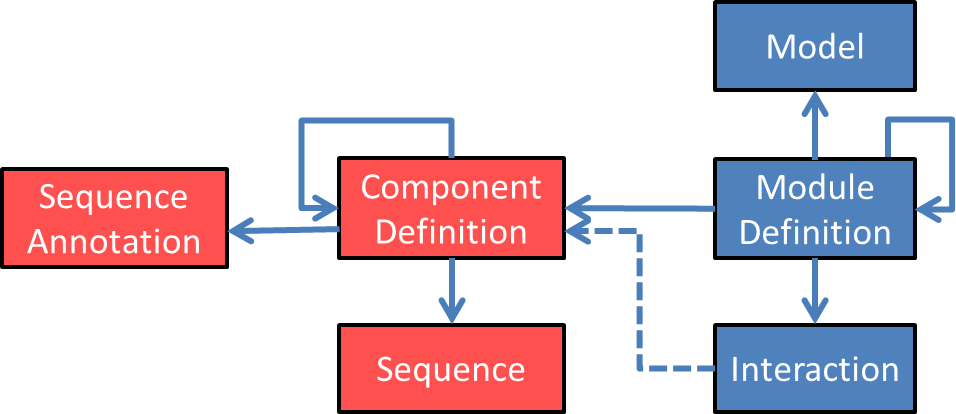
\includegraphics[scale=0.5]{images/OverviewFigforSpec-v3.png}
\caption{Main classes of information represented by the SBOL standard, and their relationships.  Red boxes are classes from the 1.1 version of SBOL that focused on structure, whereas blue classes are some of the new classes that support the functional aspects of designs.}
\label{images:overview1}
\end{center}
\end{figure}

\begin{figure}[ht]
\begin{center}
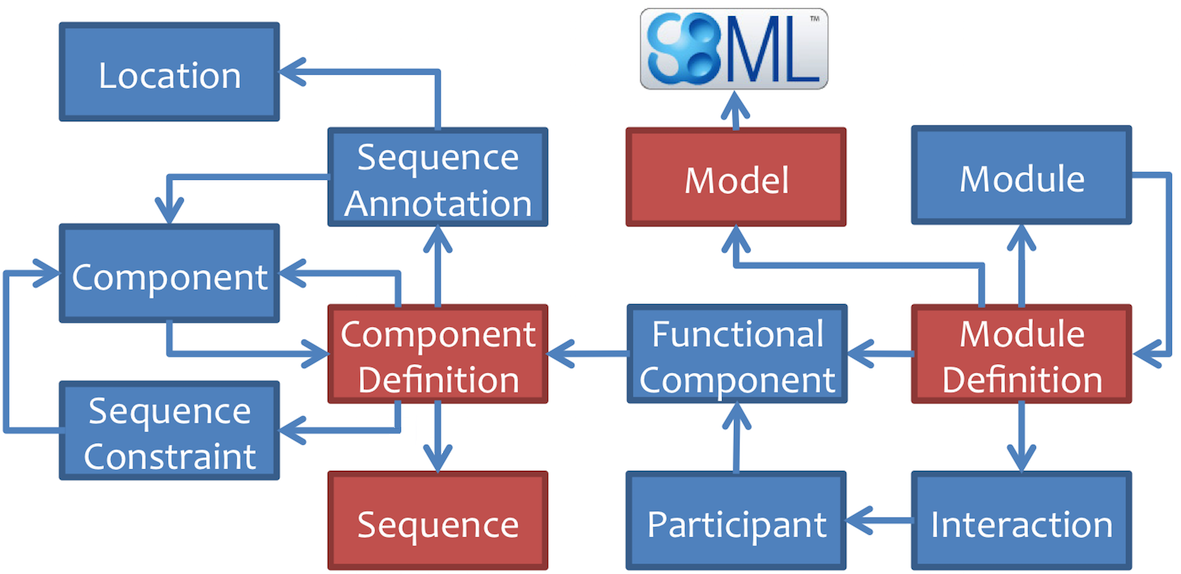
\includegraphics[scale=1.2]{images/SBOL2_2_revised.png}
\caption{Main classes of information represented by the SBOL standard, and their relationships.  Red boxes are ``top level'' classes, while blue classes are used in describing a top-level class; an arrow indicates that one class refers to another.}
\label{images:overview2}
\end{center}
\end{figure}

The \sbol{Sequence} is a fundamental information object for synthetic biology and is needed to reuse components, to replicate synthetic biology work, and to assemble new synthetic biological systems. In designed systems such objects can consist of small chemical molecules, DNAs, RNAs or Proteins. The \sbol{Sequence} object has been designed to encapsulate any of these types of molecules. Small molecule \sbol{Sequence} objects are typically referred to via their chemical formulae. Molecules where sequence specific information is important, such as DNA, RNA and Protein \sbol{Sequence} objects, use the object to incorporate this information. The \sbol{Sequence} object encapsulates this positional information as well as the associated experimental work or other information related to a sequenced molecule.

\Rtodo{need to make it clear that it includes DNA, RNA, and protein, also smooth the text --JSB made addiitons based upon the suggested changes - KC}

In the SBOL data model, a structural layer defines the physical arrangement of components in a biological system.  \sbol{ComponentDefinition}s define genetic elements such as promoters, RBSs, CDSs, and terminators, as well as RNA, proteins, and small molecules.  In a structural hierarchy, \sbol{ComponentDefinition}s can contain subcomponents (\sbol{Component}s), which are instances of the \sbol{ComponentDefinition} for that subcomponent.  A functional layer can be defined to describe the behaviors that arise from the structural layer.  \sbol{ModuleDefinition}s contain information about molecular interactions and their participating components.  They can contain \sbol{FunctionalComponent}s that are instances of \sbol{ComponentDefinition}s that can be assigned functional properties, and they can also contain other modules in a functional hierarchy.  The functions and interactions of these components and other modules within the \sbol{ModuleDefinition} can be quantitatively or qualitatively described using a \sbol{Model}. The \sbol{SequenceAnnotation} object defines data associated the \sbol{Sequence} and \sbol{ComponentDefinition} objects that is needed beyond basic definitions. This can refer to local annotations of the object as well as a container for URIs to external information sources. 


SBOL includes different entities to describe such genetic circuits. Genetic elements such as a promoter, ribosome binding site (RBS), coding sequence (CDS), or terminator are defined with the \sbol{ComponentDefinition} entity. Their instances are reused in different designs via the \sbol{Component}s that refer to corresponding \sbol{ComponentDefinition}s. \sbol{ComponentDefinition}s can also represent proteins, RNAs or small molecules. They are associated with sequence information such as nucleotides aminoacids or chemical structure. A full description of a genetic circuit is then represented using  \sbol{ModuleDefinition}s which contains information about molecular interactions and their participating components. Modules can be associated with quantitative or qualitative models using the \sbol{Model} entity, which is used to point to the actual location of a model. 
\sbol{SequenceAnnotation}s can be used to carry data associated with the successful running of that model on another computer, can be used to point towards sources of some or all of the circuit and the location of experimental data associated with the development of the model.

\Rtodo{Need to also explain annotation --JSB
Provided some text for review describing annotation - KC}



SBOL facilitates the design of complex systems using hierarchical composition. In addition to using simple genetic elements in a modular fashion, modules that are composed of multiple, different components can also be reused. Such modules can expose some of the design components as inputs and outputs, which can be connected to components from other modules using \sbol{MapsTo} entities.


\Ctodo{This needs to be clarified.  Do we really want to explain MapsTo here? -JSB}
\Ctodo{it's not in the diagram. So it should be removed or dealt with in the figure and earlier in the text- KC}

\Ctodo{Explain why it is important to separate definitions from instantiations?}

\LDtodo{The motivation for separating structural and functional considerations is not explained.  Which class names are structural, which class names are functional, and how are the two connected?  Do all structural components require a functional counterpart?  If not, explain why only a subset of structural components would have functional definitions.}

\Ctodo{As a person reading about SBOL2 for the first time, I rank this as the most important section.  While the document should be technically focused overall, this section is your chance to concisely tell someone who won't read the whole document about the take-home messages for the new data model.}

\LDtodo{Why are URI's needed for Components?  Why not just for ComponentDefinitions?  Is there anything in SBOL that does not require a URI?}
\Ctodo{Also briefly mention URI}

\Ctodo{Make sure we explain about annotations up in the motivation and overview, since it's really, really important.}

% The same toggle switch is now displayed using two LacI and TetR inverter submodules in figure \ref{images:toggleswitch_modular}. The LacI inverter uses LacI as input and produces the TetR output, and the TetR inverter uses TetR as input and produces the LacI output. These inputs and outputs are mapped in a parent module.

% Removed as redundant:
%-----------------------------------------------------------------------------
%\section{Introduction}
% -----------------------------------------------------------------------------
%While the first version of the Synthetic Biology Open Language (SBOL) has been adopted by several academic and commercial genetic design automation (GDA) software tools, it only covers a limited range of the requirements for a standardized exchange format for synthetic biology. The SBOL 2.0 specification revises version 1.1, enabling the representation of a wider range of components with and without sequences, including RNA components, protein components, small molecules, and molecular complexes. Additionally, the latest SBOL can be used to convey the intended function of a design, as well as its structural composition. 
%This dichotomous representation of the structural and functional features of a design is a paradigm applied to great success in electrical and computer engineering, and is essential for the development of design automation software in synthetic biology.
%
%The goal of this specification is to define the terminology and relationships used to describe biological designs. In order to provide a shared understanding between engineers seeking to exchange biological designs, SBOL provides a common definition of the concepts needed. As much as possible, we attempt to make explicit the meaning of all terminology and data structures.


% % -----------------------------------------------------------------------------
% \section{Overview of SBOL}
% % -----------------------------------------------------------------------------
% Typically, information about a  genetic circuit includes the order of its constituents and their descriptions. The exact locations of these constituents and their sequences allow genetic circuits to be defined unambiguously, and reused in other designs. Interactions between these constituents are then used to construct biologically plausible designs. 

% In the figure below, a simple toggle switch system is displayed, in which LacI and TetR repress each other's genes transcriptionally. The toggling of the system  is controlled by adding IPTG to deactivate LacI, and ATC to deactivate TetR. The components of the system includes genetic elements, proteins, small molecules.

% \begin{figure}[ht]
% \begin{center}
% 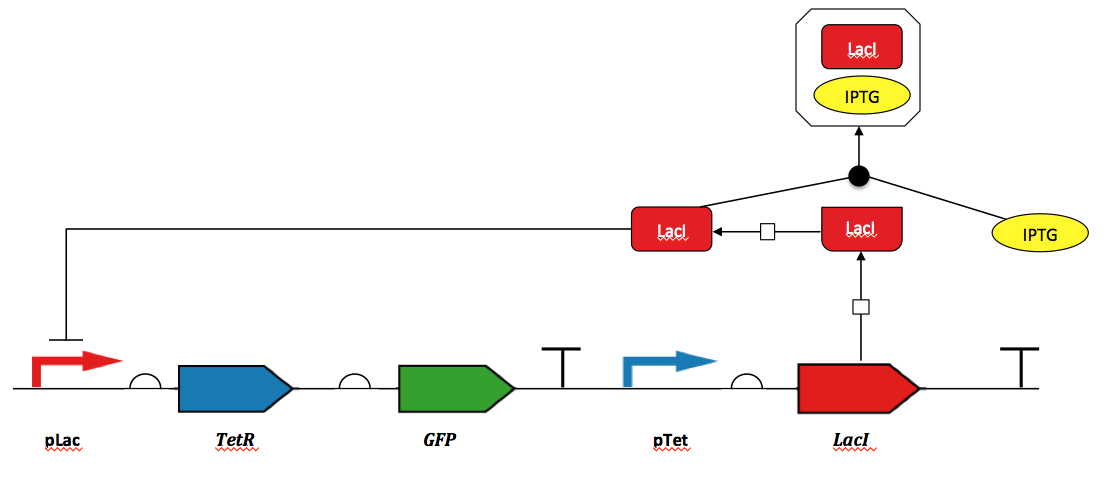
\includegraphics[scale=0.4]{images/toggleswitch_flat}
% \caption[]{An example toggle swicth genetic circuit. }
% \label{images:toggleswitch_flat}
% \end{center}
% \end{figure}

% SBOL includes different entities to describe such genetic circuits. Genetic elements such as promoters, RBS, CDSs and terminators are defined with the \sbol{ComponentDefinition} entity. Their instances are reused in different designs via the \sbol{Component}s that refer to corresponding \sbol{ComponentDefinition}s. \sbol{ComponentDefinition}s can also represent proteins, RNAs or small molecules. They are associated with sequence information such as nucleotides aminoacids or chemical structure. A full description of a genetic circuit is then represented using  \sbol{ModuleDefinition}s which contains information about molecular interactions and their participating components. Modules can be associated with quantitative or qualitative models using the \sbol{Model} entity, which is used to point to the actual location of a model.


% SBOL facilitates the design of complex systems using hierarchical composition. In addition to using simple genetic elements in a modular fashion, modules that are composed of multiple, different components can also be reused. Such modules can expose some of the design components as inputs and outputs, which can be connected to components from other modules using \sbol{MapsTo} entities.

\subsection{Model}
\label{sec:Model}

\begin{figure}[ht]
\begin{center}
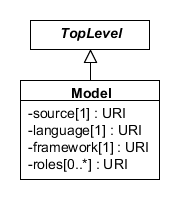
\includegraphics[scale=0.6]{uml/model}
\caption[]{Diagram of the \sbol{Model} class and its associated properties.}
\label{uml:model}
\end{center}
\end{figure}

The purpose of the \sbol{Model} class is to serve as a placeholder for an external computational model and provide additional meta-data to enable better reasoning about the contents of this model.
In this way, there is minimal duplication of standardization efforts and users of SBOL can formalize the function of a \sbol{Component} in the language of their choice.

The meta-data provided by the \sbol{Model} class include the following properties: the \sbolmult{source:M}{source} or location of the actual content of the model, the \sbol{language} in which the model is implemented, and the model's \sbol{framework}.

\subparagraph{The \sbolheading{source} property}\label{sec:source:M}
The \sbolmult{source:M}{source} property is REQUIRED and MUST contain a \sbol{URI} reference to the source file for a model.

\subparagraph{The \sbolheading{language} property}\label{sec:language}
The \sbol{language} property is REQUIRED and MUST contain a \sbol{URI} that specifies the language in which the model is implemented. It is RECOMMENDED that this \sbol{URI} refer to a term from the EMBRACE Data and Methods (EDAM) ontology. \ref{tbl:model_types} provides a list of terms from this ontology and their \sbol{URI}s. If the \sbol{language} property of a \sbol{Model} is well-described by one these terms, then it MUST contain the \sbol{URI} for this term as its value.

\begin{table}[ht]
  \begin{edtable}{tabular}{ll}
    \toprule
    \textbf{Model Language} & \textbf{URI for EDAM Term} \\
    \midrule
    SBML  & \url{http://identifiers.org/edam/format_2585}\\
    CellML		 & \url{http://identifiers.org/edam/format_3240}\\
    BioPAX    & \url{http://identifiers.org/edam/format_3156}\\
    \bottomrule
  \end{edtable}
  \caption{Terms from the EDAM ontology to specify the \sbol{language} property of a \sbol{Model}.}
  \label{tbl:model_types}
\end{table}


\subparagraph{The \sbolheading{framework} property}\label{sec:framework}
The \sbol{framework} property is REQUIRED and MUST contain a \sbol{URI} that specifies the framework in which the model is implemented.
It is RECOMMENDED this \sbol{URI} refer to a term from the modeling framework branch of the SBO when possible. A few suggested modeling frameworks and their corresponding \sbol{URI}s are shown in \ref{tbl:model_frameworks}. If the \sbol{framework} property of a \sbol{Model} is well-described by one these terms, then it MUST contain the \sbol{URI} for this term as its value.

\begin{table}[ht]
  \begin{edtable}{tabular}{ll}
    \toprule
    \textbf{Framework} & \textbf{URI for SBO Term} \\
    \midrule
    Continuous  & \url{http://identifiers.org/biomodels.sbo/SBO:0000062}\\
    Discrete & \url{http://identifiers.org/biomodels.sbo/SBO:0000063}\\
    \bottomrule
  \end{edtable}
  \caption{SBO terms to specify the \sbol{framework} property of a \sbol{Model}.}
  \label{tbl:model_frameworks}
\end{table}


% -----------------------------------------------------------------------------
\section{Data Model Examples}
\label{sec:examples}
% -----------------------------------------------------------------------------

%\subsection{LacI/TetR Toggle Switch}

This section illustrates how to use the SBOL data model by specifying the design of a LacI/TetR toggle switch similar to those constructed in \cite{Gardner2000}. This design is visualized conceptually in \ref{images:toggle} and in detail in \ref{images:toggleswitch_modular}. 

Conceptually, the toggle switch is constructed from two mutually repressing genes.  
With repressors LacI and TetR, this results in a bi-stable system that will tend to settle into a state where precisely one of the two repressors is strongly expressed, repressing the other.
Each of these repressors can have its activity disrupted by a small molecule (IPTG for LacI, aTc for TetR), which allows the system to be ``toggled'' from one state to the other by dosing it with the appropriate small molecule.

\begin{figure}[ht]
\begin{center}
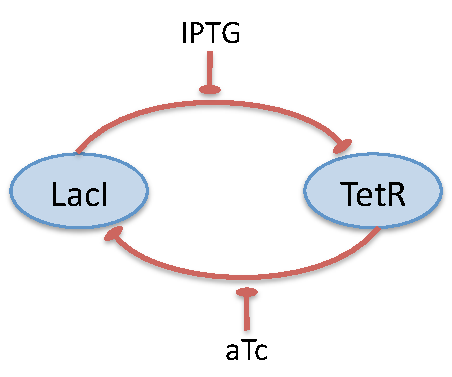
\includegraphics[scale=1.0]{images/toggle-highlevel.pdf}
\caption[]{Conceptual diagram of LacI/TetR toggle switch: the LacI 
  and TetR transcriptional factors are arranged to mutually repress, 
  creating a bi-stable system.  Transition between the two states
  is triggered by the small-molecule signals aTc (which disrupts TetR
  repression) and IPTG (which disrupts LacI repression).}
\label{images:toggle}
\end{center}
\end{figure}

\begin{figure}[ht]
\begin{center}
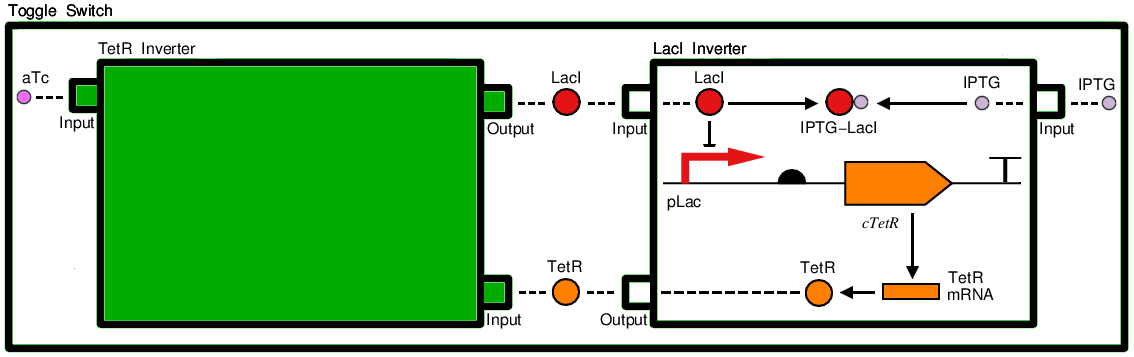
\includegraphics[scale=0.4]{images/toggleswitch_modular}
\caption[]{Design of a LacI/TetR toggle switch. This design is composed of two inverter sub-designs, each containing a single gene. These genes mutually repress each other's expression via their encoded protein transcription factors, LacI and TetR. Furthermore, both LacI and TetR are bound by specific small molecules that sequester them and prevent them from acting as repressors. In this design, arrows represent different molecular interactions, including the repression of pLac via LacI, the non-covalent binding of IPTG to LacI, the transcription of TetR mRNA, and the translation of TetR. Dashed lines serve to map between transcription factors in the inverter sub-designs and those in the overall toggle switch design.}
\label{images:toggleswitch_modular}
\end{center}
\end{figure}

The LacI/TetR toggle switch is modeled in SBOL as two parallel hierarchies of structure and function. The structural hierarchy of the toggle switch is represented using \sbol{ComponentDefinition}s:
\begin{itemize}
\item The base elements of the hierarchy are DNA components, transcription factor proteins, and small molecules. As an example, \ref{uml:ex_comp_defs} is a UML diagram of the \sbol{ComponentDefinition}s that represent these elements.
\item Base elements are composed to form more complex structures at the top of the hierarchy, including genes and non-covalent complexes between transcription factor proteins and small molecules. As an example, \ref{uml:ex_comp_def_compo} is a UML diagram of the composite \sbol{ComponentDefinition}s that represent the TetR gene and IPTG-LacI complex.
\end{itemize}

\begin{figure}[ht]
\begin{center}
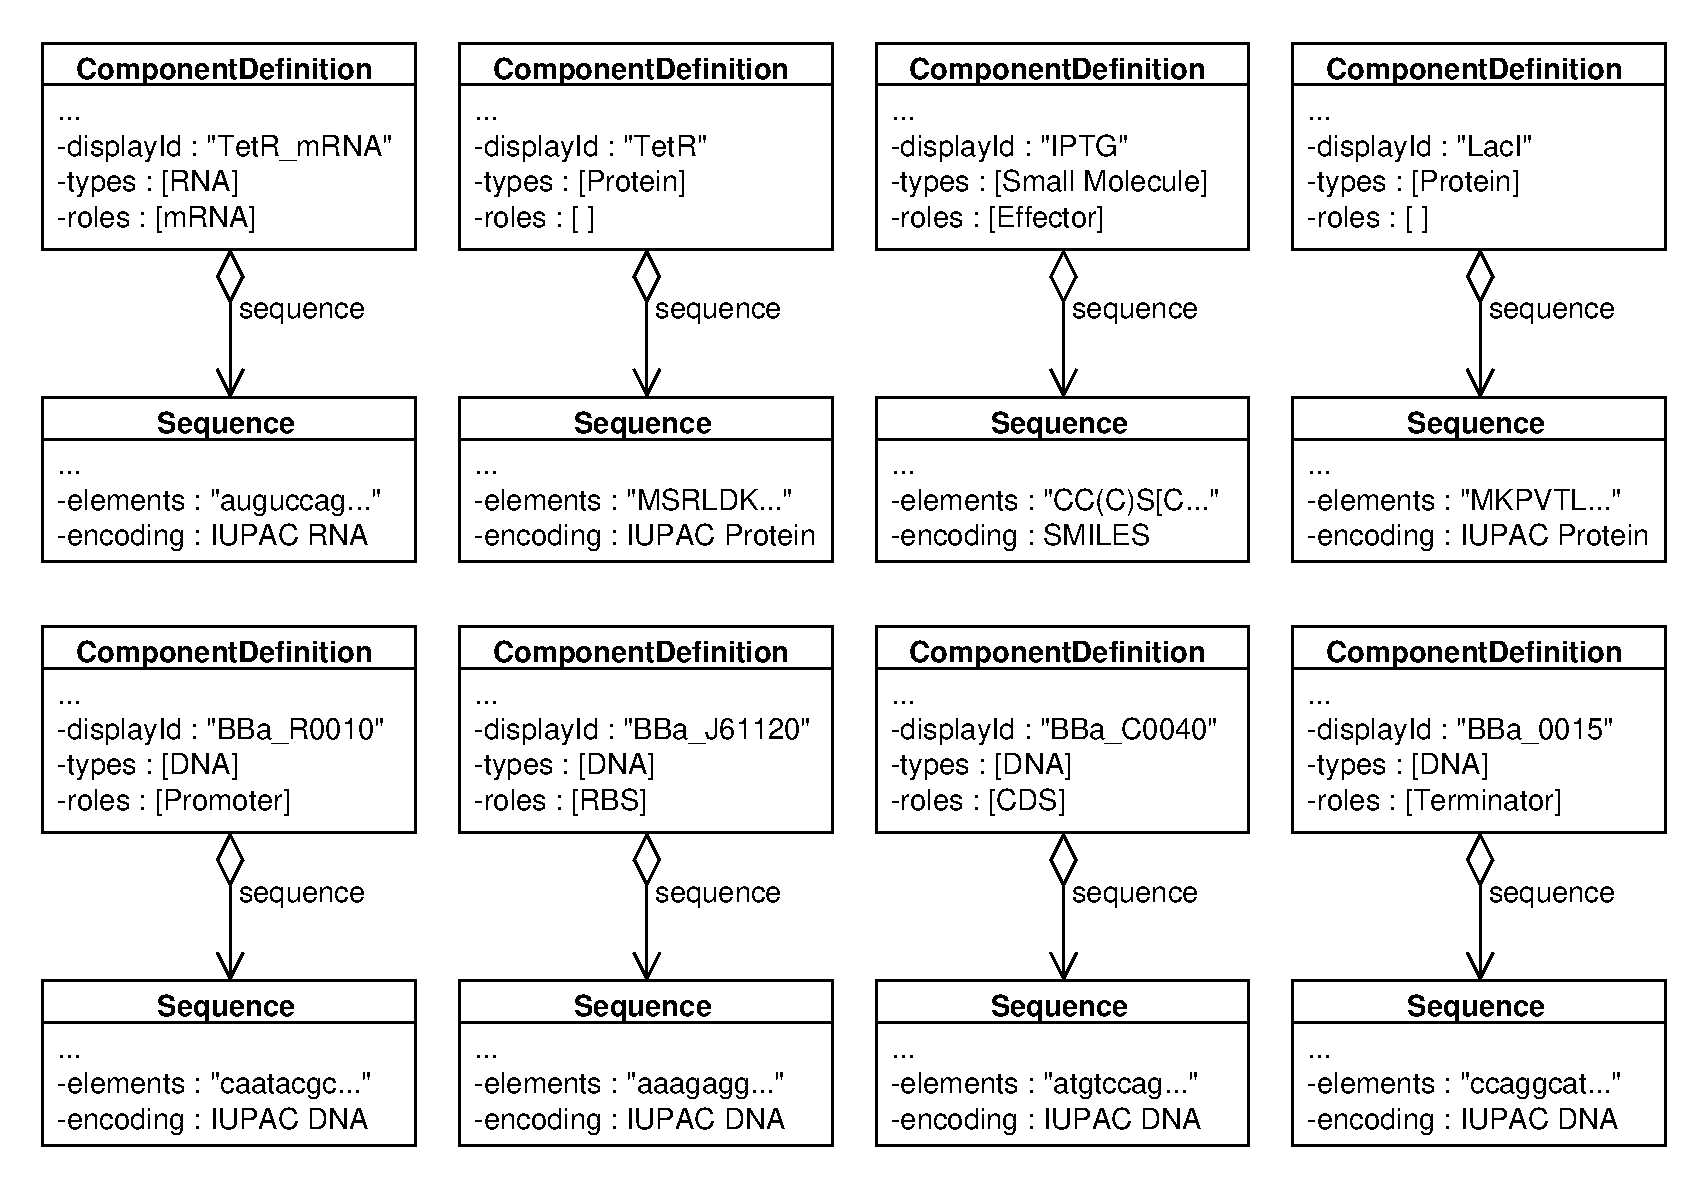
\includegraphics[width=\textwidth]{example_uml/toggle_1}
\caption[]{\sbol{ComponentDefinition} objects for the LacI inverter. These include \sbol{ComponentDefinition} objects based on DNA parts from the iGEM Registry and  \sbol{ComponentDefinition}s that represent TetR mRNA, TetR, LacI, and and IPTG. Each \sbol{ComponentDefinition} is associated with a \sbol{Sequence} that has an \external{IUPAC DNA/RNA} or \external{IUPAC protein} \sbol{encoding}, except the \sbol{ComponentDefinition} of IPTG, which is associated with a \sbol{Sequence} that has a \external{SMILES} \sbol{encoding}.}
\label{uml:ex_comp_defs}
\end{center}
\end{figure}

\begin{figure}[ht]
\begin{center}
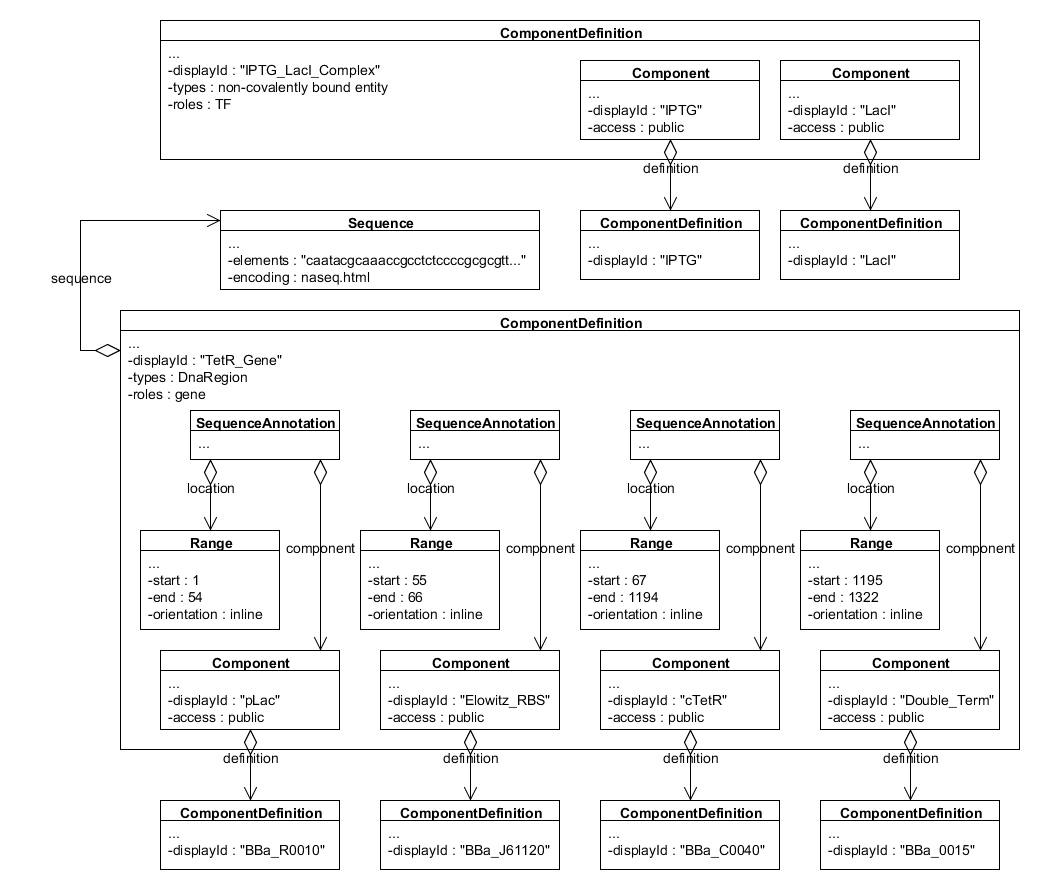
\includegraphics[width=\textwidth]{example_uml/toggle_2}
\caption[]{Composite \sbol{ComponentDefinition} objects for the LacI inverter. In the case of the \sbol{ComponentDefinition} that represents the TetR gene, its sub-\sbol{Component} objects are located as \sbol{Range}s along its \sbol{Sequence} using \sbol{SequenceAnnotation}s. The \sbol{ComponentDefinition} that represents the IPTG-LacI complex, however, has no \sbol{Sequence} and its sub-\sbol{Component} objects are composed without any data about their relative positions.}
\label{uml:ex_comp_def_compo}
\end{center}
\end{figure}

The functional hierarchy of the toggle switch is represented using
\sbol{ModuleDefinition}s:
\begin{itemize}
\item The base elements of the hierarchy are LacI-dependent repression of TetR expression (the LacI inverter) and TetR-dependent repression of LacI (the TetR inverter). As an example, \ref{uml:ex_mod_def} is a UML diagram of the \sbol{ModuleDefinition} that represents the LacI inverter.
\item Base elements are composed to form the toggle switch at the top of the hierarchy.  As an example, \ref{uml:ex_mod_def_compo} is a UML diagram of the \sbol{ModuleDefinition} that represents the toggle switch.
\end{itemize}

\begin{figure}[ht]
\begin{center}
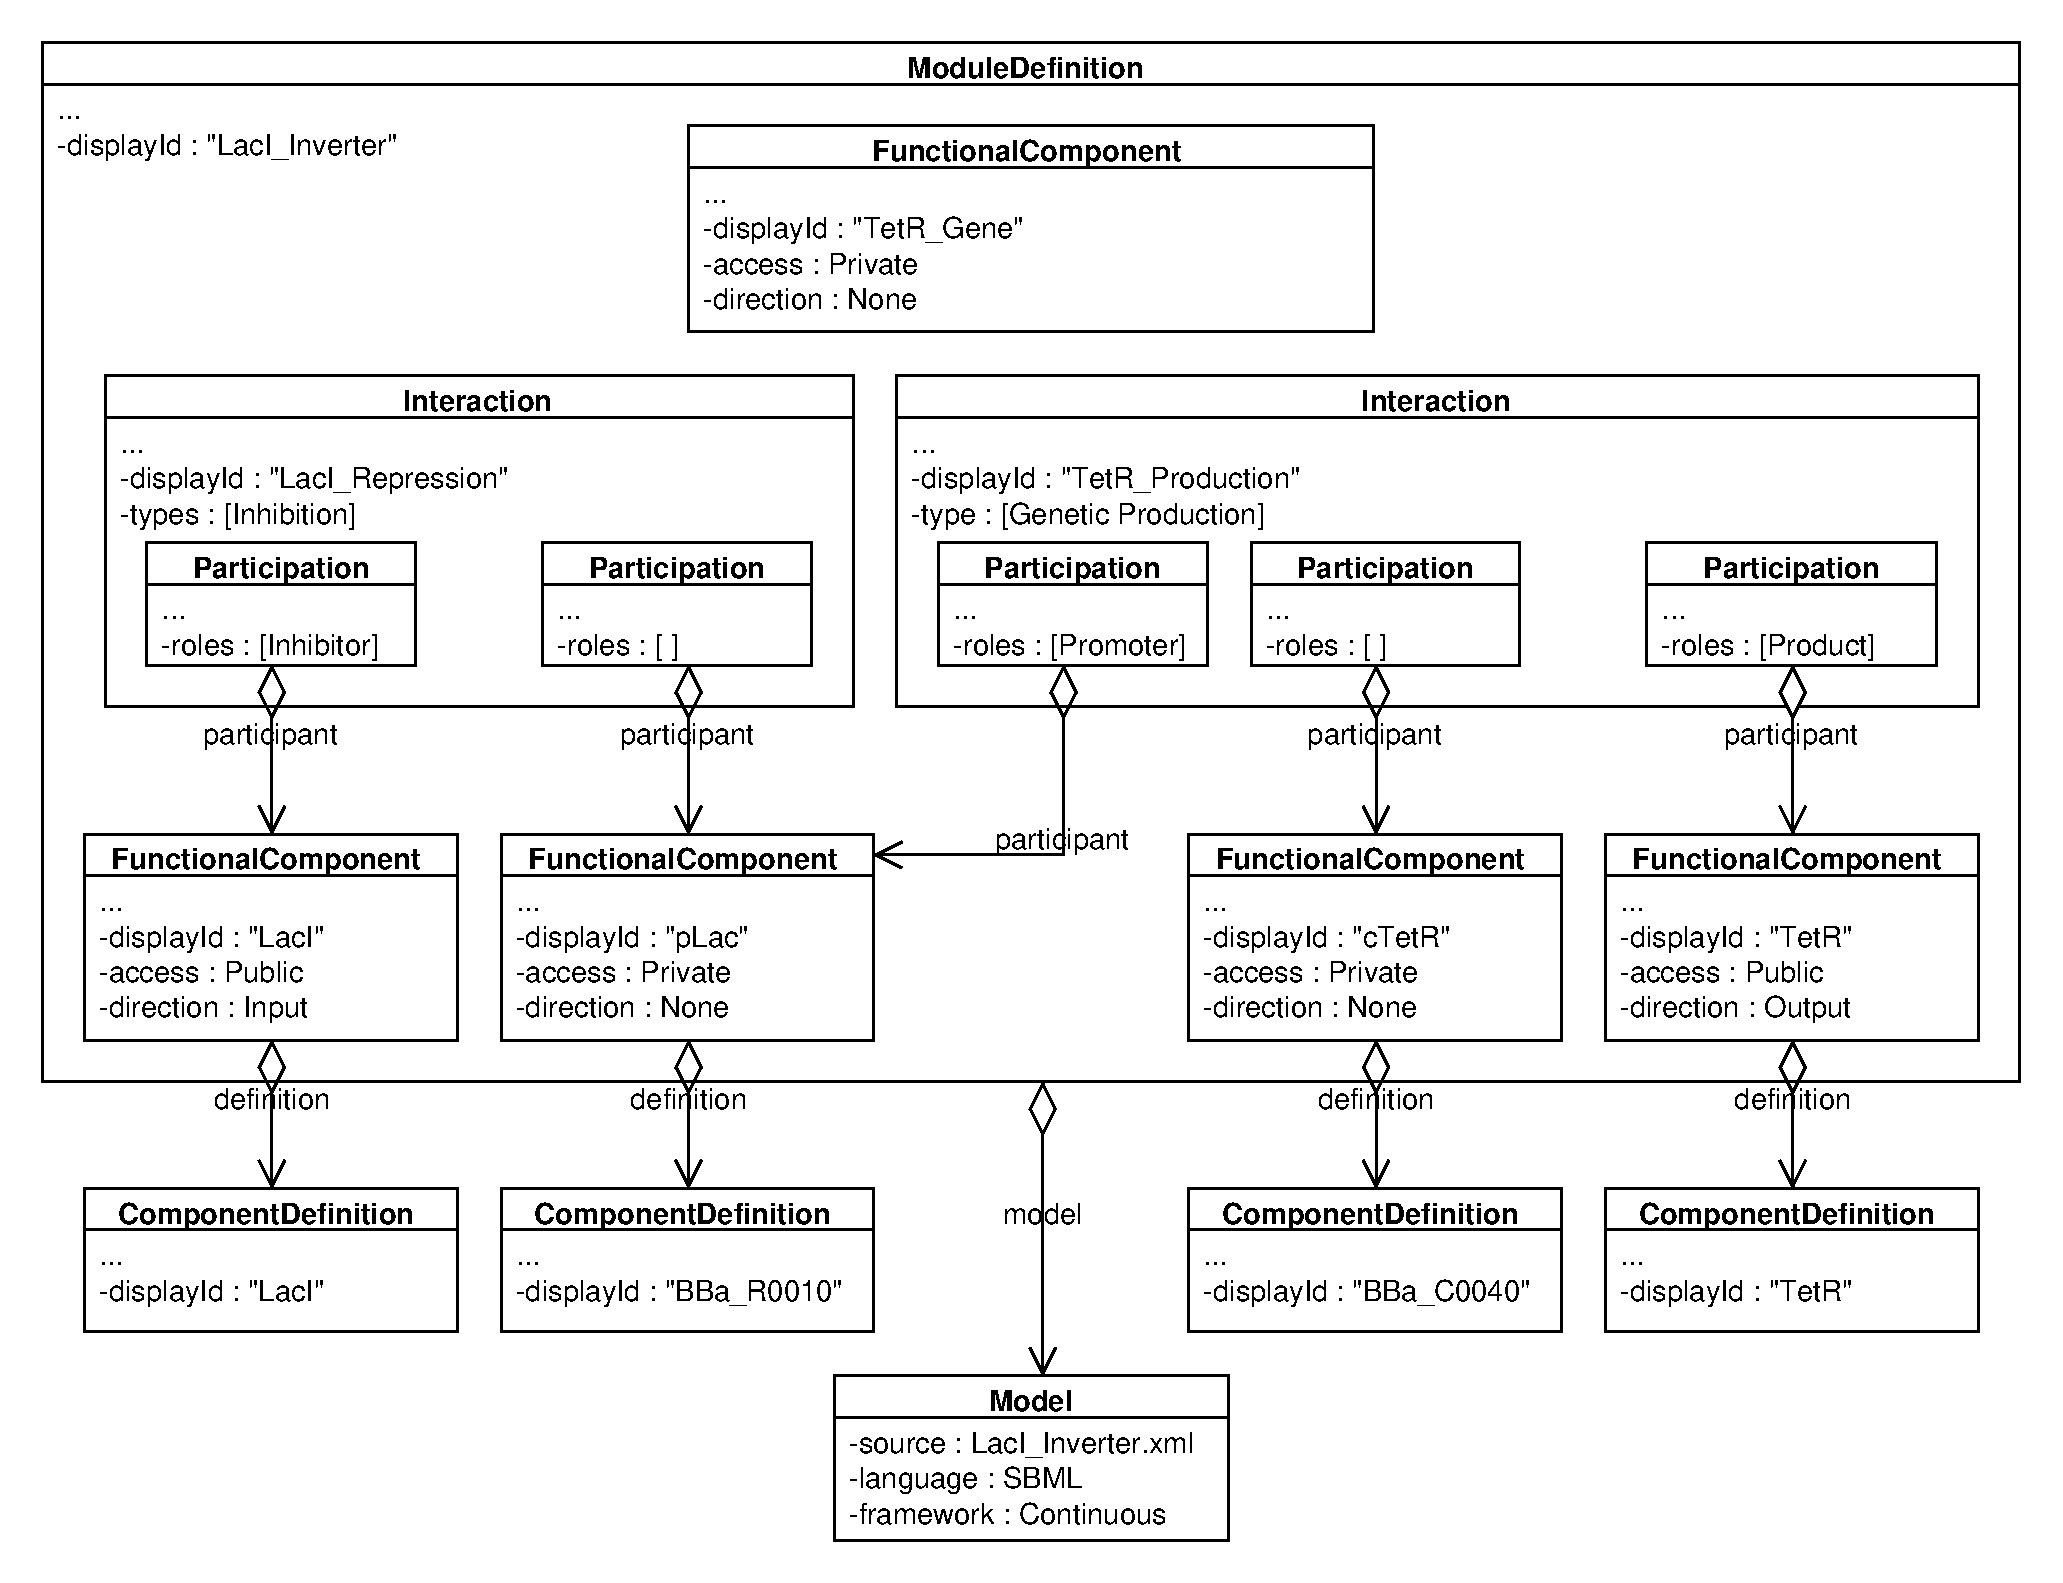
\includegraphics[width=\textwidth]{example_uml/toggle_3}
\caption[]{\sbol{ModuleDefinition} of the LacI inverter. This \sbol{ModuleDefinition} contains \sbol{FunctionalComponent} objects that instantiate the \sbol{ComponentDefinition} objects for the LacI/TetR transcription factors and TetR gene. The \sbol{FunctionalComponent} for the TetR gene as a whole does not participate in any \sbol{Interaction} and merely indicates the overall structure that is functionally described by the LacI inverter \sbol{ModuleDefinition}. The remaining \sbol{FunctionalComponent} objects participate in a repression \sbol{Interaction} and a genetic production \sbol{Interaction}, thereby indicating which parts of the overall structure carry out the function of the LacI inverter \sbol{ModuleDefinition}. In this case, the transcription and translation of TetR are represented as a single genetic production \sbol{Interaction} that abstracts away the presence of the intermediate TetR mRNA.  In addition, this \sbol{ModuleDefinition} is also associated with a continuous \sbol{Model} written in the SBML source file ``LacI\_Inverter.xml.''}
\label{uml:ex_mod_def}
\end{center}
\end{figure}

\begin{figure}[ht]
\begin{center}
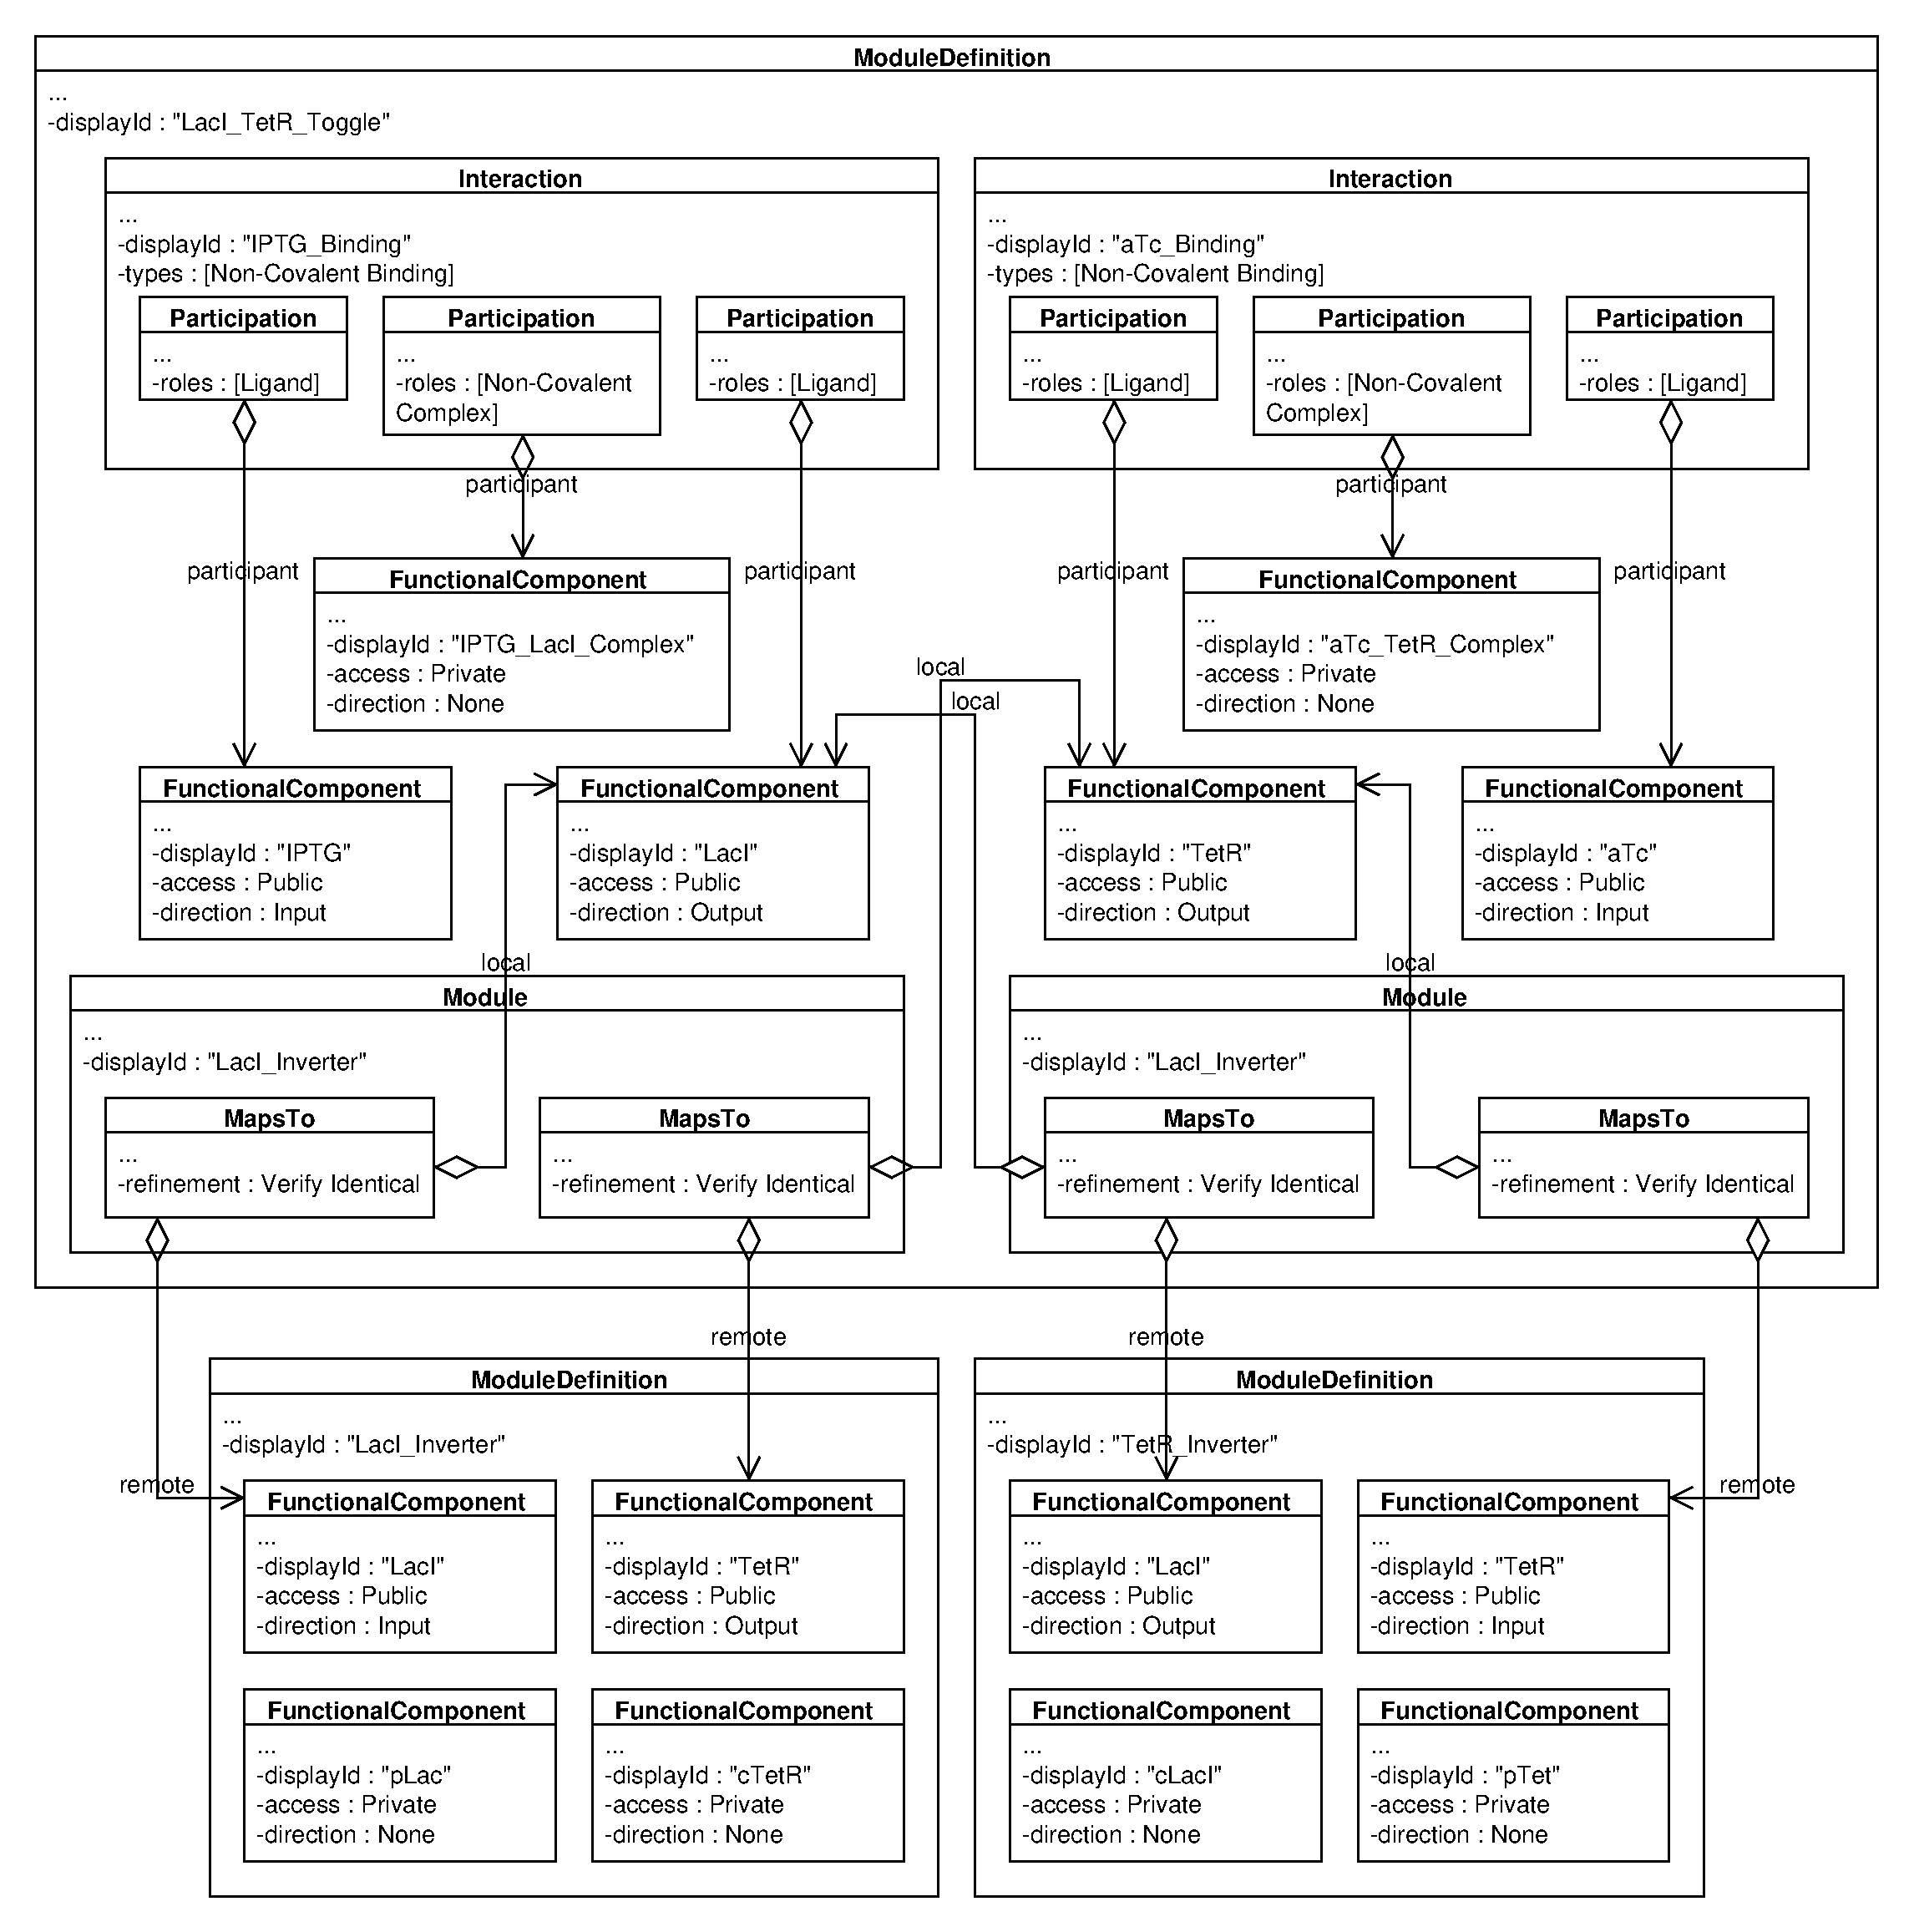
\includegraphics[width=\textwidth]{example_uml/toggle_4}
\caption[]{Composite \sbol{ModuleDefinition} of the LacI/TetR toggle switch. This \sbol{ModuleDefinition} contains the \sbol{Module} objects that instantiate \sbol{ModuleDefinition} object for sthe LacI and TetR inverter. It also contains \sbol{FunctionalComponent} objects that instantiate the \sbol{ComponentDefinition} objects for the LacI/TetR transcription factors and IPTG/aTc small molecules. These \sbol{FunctionalComponent} objects each participate in a non-covalent binding \sbol{Interaction}. To complete the composition of the toggle switch, \sbol{MapsTo} objects are used to indicate that the output of the LacI inverter \sbol{ModuleDefinition} is identical to the input of the TetR inverter \sbol{ModuleDefinition} and vice versa.
}
\label{uml:ex_mod_def_compo}
\end{center}
\end{figure}

% Each \sbol{ModuleDefinition} also contains the \sbol{FunctionalComponent}s that participate in \sbol{Interaction}s and are defined by the same \sbol{ComponentDefinition}s as the parallel \sbol{Component}s in the structural hierarchy of the toggle switch. Finally, \sbol{MapsTo} entities are used to refine which \sbol{FunctionalComponent}s of the functional hierarchy are identical or map them to \sbol{Component}s in the structural hierarchy.

\Rtodo{ComponentDefinition.types in the following figure are not consistent with the list of BioPax ontological terms described previously in the Data Model section. Should now be consistent. - Nic}

%  The first use case is to indicate with greater fidelity how a module describes the function of a composite component, namely by asserting that particular component instantiations within the module correspond to particular component instantiations within the component. 

% As an example of this use case, one might compose the structure and function of the LacI-repressible gene of the genetic toggle switch. In this example, the LacI-repressible gene and two of its subcomponents, the pLac promoter and cTetR CDS, are to be composed with the LacI inverter module. In order to compose these components with the LacI inverter module and indicate that it describes their behavior, they are instantiated inside the module. In addition, port maps are placed on the instantiation of the LacI-repressible gene to connect between its pLac plus cTetR subcomponent instantiations and the corresponding component instantiations in the module. Doing so makes it clear which subcomponent instantiations in the gene are being described by which component instantiations in the module. In this way, GDA tools for sequence editing and biochemical modeling can guarantee that their users are handling corresponding elements of a given genetic design, while GDA tools for genetic technology mapping can make explicit connections between the structural and functional elements of a design.

% -----------------------------------------------------------------------------
\section{SBOL RDF Serialization}
\label{sec:serialization}
% -----------------------------------------------------------------------------

\todo[inline]{try to target readers unfamiliar with RDF/XML.  -bder}

The SBOL serialization is designed to meet several competing requirements. Firstly, SBOL needs to support ad-hoc annotations and extensions. Secondly, SBOL needs to support processing by generic semantic web and database tools that have little or no knowledge of the SBOL data model. Thirdly, SBOL needs to support the generation of light-weight software clients so as to lower the barrier to entry for new API implementations within environments where community-maintained implementation(s) are not suitable.

The canonical serialization of SBOL is to a strict dialect of RDF/XML. This serialization provides the base from which to meet further requirements. Any RDF/XML-aware tooling can consume and analyze an SBOL file. Where possible, we have re-used predicates from widely-used terminologies (such as Dublin Core~\cite{dcmi2012}) to expose as much of the data as practical to standard RDF tooling.

Arbitrary RDF/XML provides a great deal of flexibility in how equivalent data can be serialized. This flexibility can result in different serializations when processing RDF/XML files using standard off-the-shelf XML tools, such as DOM-OO mappings. To address this problem, we define a canonical association between the nesting of data structures within the SBOL UML data model and the RDF/XML file. For all ownership associations (filled diamonds), the RDF/XML for the owned entity is embedded within the owner's RDF/XML. For all associations that are by reference (open diamonds), the RDF/XML for the referenced property is linked via a resource URI.

All first-class SBOL datatypes have an associated identity URI. In the RDF, this is the resource URI used by instances of that type. Properties and associations are asserted as nested RDF/XML assertions. Some datatypes are `top level,' which means that they always appear at the top level of the RDF/XML serialization. All other datatypes will always appear nested within their parent container.

Each instance of a first-class SBOL datatype may have annotations attached. These annotations are composed of a name and a value.  They are serialized to RDF as a triple with the subject being the identity of the instance they annotate, the predicate being the name of the annotation, and the object being the value of that annotation. Annotation values are always nested within the RDF/XML serialization of the instance that they annotate.

SBOL supports top-level, user-defined annotations. This is to allow non-standardized but necessary information to be carried around as part of a design. For example, a particular sub-community may have an internal standard for data sheets. Individual data sheets can be represented as a generic top-level annotation with internal structured annotations. This annotation will be serialized into the RDF/XML in the usual way, as a RDF/XML block at the top level of the file. Other objects may refer to this entity through their annotations by reference, and this generic top-level entity may refer to other entities via references.

By adopting this paradigm of RDF/XML serialization, SBOL is able to adapt to future changes in the standard without requiring large-scale alterations to the RDF files. Since exactly the same scheme is used to serialize annotations as is used to serialize specification-defined properties and associations, it is possible to update the SBOL standard to recognize a different range of properties and associations. Those properties not recognized by the specification will always be available through the API as annotations. Similarly, by allowing arbitrary top-level entities in an SBOL file, we enable future specifications or extensions to ratify the structure of . These entities would then become part of the explicit data model, but the identical RDF serialization would be used. Applications lacking support for a given extension can safely round-trip the top-level data that is not understood, treating it as a top-level structured annotation, without data loss or corruption. The very regimented control of nesting versus referencing allows the XML structure to be very predictable, enabling XML/DOM-based tooling to work with SBOL RDF/XML files safely.


\section{SBOL Compliance}

There are different types of software compliance with respect to the SBOL specification.  First, a software tool can either support all classes of the SBOL 2.x data model or only its structural subset.  The structural subset includes the following classes:
\begin{itemize}
\item \sbol{Sequence}
\item \sbol{ComponentDefinition}
\begin{itemize}
\item \sbol{Component}
\item \sbol{SequenceAnnotation}
\item \sbol{SequenceConstraint}
\end{itemize}
\item \sbol{Collection}
\item \sbol{Annotation}
\item \sbol{GenericTopLevel}
\end{itemize}
Second, an SBOL-compliant software tool can support import of SBOL, export of SBOL, or both.  
If it supports both import and export, it can do so in either a lossy or lossless fashion.

In order to test import compliance, developers are encouraged to use the SBOL test files found here:\\ {\url{https://github.com/SynBioDex/SBOLTestSuite}}\\
Examples of every meaningful subset of objects are provided, including both structural-only SBOL (that is, annotated DNA sequence data) and complete tests.  

In order to test export compliance, developers are encouraged to validate SBOL files generated by their software with the SBOL Validator found here:\\
\url{http://www.async.ece.utah.edu/sbol-validator/}\\
This validator can also be used to check lossless import/export support, since it can compare the data content of files imported and exported by a software tool.

Finally, developers of SBOL-compliant tools are encouraged to notify the SBOL editors\\(sbol-editors@googlegroups.com) when they have determined that their tool is SBOL compliant, so their tool can be publicly categorized as such on the SBOL website.




% -----------------------------------------------------------------------------
\section{Recommended Best Practices}
\label{sec:bestpractices}
% -----------------------------------------------------------------------------
\subsection{SBOL Versions}

To differentiate between major versions of SBOL, different namespaces are used.  For example, SBOL3 has the namespace \url{http://sbols.org/v3#}, while SBOL2 has the namespace \url{http://sbols.org/v2#}.  These different versions of SBOL SHOULD NOT be semantically mixed. For example, an SBOL 3.x \sbol{SubComponent} SHOULD NOT refer to an SBOL 2.x \external{ComponentInstance}, and, likewise, an SBOL 2.x \external{ComponentInstance} SHOULD NOT refer to an SBOL 1.x \external{DnaComponent}.

\subsection{Compliant SBOL Objects}
\label{sec:compliant}

Maintaining unique URIs for all SBOL objects can be challenging.  To reduce this burden, users of SBOL 3.x are encouraged to follow a few simple rules when constructing the URIs and related properties for SBOL objects.  When these rules are followed in constructing an SBOL object, we say that this object is \emph{compliant}. These rules are as follows:

Compliant URIs for \sbol{TopLevel} objects MUST conform to the following pattern:
\begin{quotation} 
\refObj{namespace}/\refObj{collection\_structure}/\refObj{displayId}
\end{quotation}

The \refObj{namespace} token MAY further decompose into \refObj{domain}/\refObj{root} tokens. The \refObj{root} and \refObj{collection\_structure} tokens may optionally be omitted; alternatively, they may consist of an arbitrary number of delimiter-separated layers. Note that this pattern means that SBOL-compliant \sbol{URI}s can be automatically decomposed with the aid of a \sbol{Namespace}. SBOL-compliant objects can be easily remapped into new namespaces by changing only the \refObj{namespace}.

Consider, for example, the SBOL-compliant \sbol{URI}:
\begin{quote}``https://synbiohub.org/igem/2017\_distribution/promoters/constitutive/BBa\_J23101''\end{quote} 
in \sbol{Namespace} ``https://synbiohub.org/igem/2017\_distribution''.
This \sbol{URI} can be decomposed as follows:
\begin{quote} 
namespace: ``https://synbiohub.org/igem/2017\_distribution'' \linebreak
domain: ``https://synbiohub.org'' \linebreak
root: ``igem/2017\_distribution'' \linebreak
collection: ``promoters/constitutive'' \linebreak
displayId: ``BBa\_J23101'' \linebreak
\end{quote}

SBOL-compliant URIs also facilitate auto-construction of child objects with unique \sbol{URI}s. 
Child objects of \sbol{TopLevel} objects with compliant \sbol{URI}s MUST conform to the following pattern:\\ ``\refObj{parent\_uri}/\refObj{child\_type}\refObj{child\_type\_counter}'' where the \refObj{parent\_uri} refers to the URI of the parent object, the \refObj{child\_type} refers to the SBOL class of the child object, and \refObj{child\_type\_counter} is a unique index for the child object. 
The \refObj{child\_type\_counter} of a new object SHOULD be calculated at time of object creation as 1 + the maximum \refObj{child\_type\_counter} for each \refObj{child\_type} object in the parent (e.g., ``\refObj{parent\_uri}/SequenceAnnotation37''). 
Note that numbering is independent for each type, so a \sbol{Component} can have children ``SubComponent37'' and ``Constraint37''.

All examples in this specification use compliant \sbol{URI}s.

\subsection{Versioning SBOL Objects}

SBOL 3.x does not specify an explicit versioning scheme. Rather it is left for experimentation across different tools. This allows version information to be included in the root (e.g., GitHub style: ``igem/HEAD/''), collection structure (e.g., ``promoters/constitutive/2/''), in tool-specific conventions on \sbol{displayId} (e.g., ``BBa\_J23101\_v2'') or in information outside of the \sbol{URI} (e.g., by attaching \external{prov:wasRevisionOf} properties).

\subsection{Annotations: Embedded Objects vs. External References}

When annotating an SBOL document with additional information, there are
two general methods that can be used:
\begin{itemize}
\item Embed the information in the SBOL document using properties outside of the SBOL namespace.
\item Store the information separately and annotate the SBOL document with \sbol{URI}s that point to it.
\end{itemize}
In theory, either method can be used in any case. (Note that a third case not
discussed here is to annotate external objects with links
to SBOL documents, rather than annotating SBOL documents with links to external objects.)

In practice, 
embedding large amounts of non-SBOL data into SBOL documents is likely
to cause problems for people and software tools trying to manage and
exchange such documents.  Therefore, it is RECOMMENDED that small amounts of information (e.g., design notes or preferred graphical layout) be embedded in the SBOL model, while large amounts of information (e.g., the contents of the scientific publication from which a model was derived or flow cytometry data that characterizes performance) be linked with URIs pointing to external resources.  The boundary between ``small'' and ``large'' is left deliberately vague, recognizing that it will likely depend on the particulars of a given SBOL application.

\subsection{Completeness and Validation}

RDF documents containing serialized SBOL objects might or might not be
entirely self-contained.  A SBOL document is self-contained or ``complete'' if every SBOL object referred to in the document is contained in the document.  It is RECOMMENDED that serializations be complete whenever practical.  In order words, when serializing an SBOL object, serialize all of the other objects that it points to, then serialize all of the other objects that these objects point to, etc., until the document is complete.

It is important to note that there is no guarantee that an RDF document
contains valid SBOL. When SBOL objects are read from an RDF document,
 the program doing so SHOULD verify that all of the property
values encoded therein have the correct data type (e.g., that the object
pointed to by the \sbol{Sequence} property of a
\sbol{Component} is really a \sbol{Sequence}).
For complete files, this validation can be carried out entirely locally. For files that are not complete, an implementation either needs to have a means of validating those external references (e.g., by
retrieving them from a repository), or it needs to mark them as
unverified and not depend on their correctness.

\subsection{Recommended Ontologies for External Terms}
\label{sec:recomm_ontologies}

External ontologies and controlled vocabularies are an integral part of SBOL. SBOL uses \sbol{URI}s to access existing biological information through these resources. 
New SBOL-specific terms are defined only when necessary. 
For example, \sbol{Component} \sbolmult{type:C}{type}s, such as DNA or protein, are described using Systems Biology Ontology (SBO) terms. Similarly, the \sbolmult{role:C}{role}s of a DNA or RNA \sbol{Component} are described via Sequence Ontology (SO) terms. Although RECOMMENDED ontologies have been indicated in relevant sections where possible, other resources providing similar terms can also be used. A summary of these external sources can be found in \ref{tbl:preferred_external_resources}.

\begin{table}[htp]
  \begin{edtable}{tabular}{p{2cm}p{1.5cm}p{5cm}p{6cm}}
    \toprule
    \textbf{SBOL Entity} & \textbf{Property} & \textbf{Preferred External Resource}
    & \textbf{More Information} \\
    \midrule
    \textbf{Component}  & type & SBO (physical entity branch)& \url{http://www.ebi.ac.uk/sbo/main/}\\
                                  & type & SO (nucleic acid topology)& \url{http://www.sequenceontology.org}\\
    						   	  & role & SO (\textit{DNA} or \textit{RNA}) & \url{http://www.sequenceontology.org}   \\
    						   	  & role & CHEBI (\textit{small molecule}) & \url{https://www.ebi.ac.uk/chebi/}   \\
							  & role & PubChem (\textit{small molecule}) & \url{https://pubchem.ncbi.nlm.nih.gov/} \\
    						   	  & role & UniProt (\textit{protein}) & \url{https://www.uniprot.org/}  \\   
    						   	  & role & NCIT (\textit{samples}) & \url{https://ncithesaurus.nci.nih.gov/}  \\   
    \textbf{Interaction}	      & type & SBO (occurring entity branch) & 
    \url{http://www.ebi.ac.uk/sbo/main/} \\
    \textbf{Participation}	      & role & SBO (participant roles branch) &
    \url{http://www.ebi.ac.uk/sbo/main/} \\
    \textbf{Model}	      		  & language & EDAM & \url{http://bioportal.bioontology.org/ontologies/EDAM}     \\
    				      		  & framework & SBO (modeling framework branch) &
    \url{http://www.ebi.ac.uk/sbo/main/} \\
    \textbf{om:Measure}	& type & SBO (systems description parameters) &
    \url{http://www.ebi.ac.uk/sbo/main/} \\
    \bottomrule
  \end{edtable}
  \caption{Preferred external resources from which to draw values for various SBOL properties.}
  \label{tbl:preferred_external_resources}
\end{table}

The URIs for ontological terms SHOULD come from identifiers.org.  However, it is acceptable to use terms from purl.org as an alternative, for example when RDF tooling requires URIs to be represented as compliant QNames.  SBOL software may convert between these forms as required.

\subsection{Annotating Entities with Date \& Time}\label{sec:DateTime}

Entities in an SBOL document can be annotated with creation and modification dates. It is RECOMMENDED that predicates, or properties, from DCMI Metadata Terms SHOULD be used to include date and time information. The \texttt{created} and \texttt{modified} terms SHOULD respectively be used to annotate SBOL entities with creation and modification dates. Date and time values SHOULD be expressed using the XML Schema \texttt{DateTime} datatype~\citep{Biron2004}. For example, ``\texttt{2016-03-16T20:12:00Z}'' specifies that the day is 16 March 2016 and the time is 20:12pm in UTC (Coordinated Universal Time).

\subsection{Annotating Entities with Authorship information}\label{sec:Authorship}

Authorship information should ideally be added to \sbol{TopLevel} entities where possible. It is RECOMMENDED that the \texttt{creator} DCMI Metadata term SHOULD be used to annotate SBOL entities with authorship information using free text. This property can be repeated for each author.
%The example below shows the use of this property for two authors and the values shown are free text \texttt{String} literals.

\subsection{Host Context / Ontologies for Experiments}

\subsubsection{Mixtures via Components}

Any \sbol{Component} can be interpreted as specifying a mixture of the material entity (SBO:0000240) \sbol{Feature}s that it includes.  The amount of each such instance included in the mixture SHOULD be specified by attaching a \om{Measure} with a \sbolmult{type:Measure}{type} set to the appropriate SBO term. The SBO terms that are RECOMMENDED as appropriate are members of the Systems Description Parameter (SBO:0000545) branch of SBO. Examples include:
\begin{itemize}
\item SBO:0000540: fraction of an entity pool (e.g., 1/3 CHO cells, 2/3 HEK cells)
\item SBO:0000472: molar concentration of an entity (e.g., 1 mM Arabinose)
\item SBO:0000361: amount of an entity pool (e.g., 200 uL M9 media)
\end{itemize}

Mixtures MAY be defined recursively, as mixtures of mixtures of mixtures, etc.

\subsubsection{Media, Inducers, and Other Reagents}

Each reagent, whether ``atomic'' (e.g., rainbow bead control) or mixture (e.g., M9 media), SHOULD be represented as a \sbol{Component}.

The roles of reagents may vary in context: for example, Arabinose may serve as an inducer or as a media carbon source. As such, role SHOULD be indicated by an NCI Thesaurus (NCIT) term in a \sbolmult{role:F}{role} property of the \sbol{SubComponent}. Examples include:
\begin{itemize}
\item NCIT:C64356: Positive Control
\item NCIT:C48694: Cell
\item NCIT:C85504: Media
\item NCIT:C14419: Strain
\item NCIT:C120268: Inducer
\end{itemize}

For more information on representing cells, strains, plasmids, and genomes, see \ref{bp:cells}

%\todo[inline]{Should we switch the GO term recommendation below to match the NCIT recommendation below?}

\subsubsection{Samples}

A complete specification of a sample SHOULD be a \sbol{Component} that includes at least:
\begin{itemize}
\item A \sbol{SubComponent} instantiating each strain in the sample
\item A \sbol{SubComponent} for the media or buffer
\item A \sbol{SubComponent} for each additional reagent added to the media (e.g., inducers, antibiotics)
\item \om{Measure}s on each of these specifying the amount in the sample
\item \om{Measure}s on the \sbol{Component} for each environmental parameter (e.g., temperature, pH, culturing time)
\end{itemize}

\subsubsection{Other Experimental Parameters}

In order to deal with parameters associated with the context in general but not specific instances, e.g., temperature, pH, total sample volume, the \sbol{hasMeasure} property of \sbol{Identified} can be used.  The \sbol{hasMeasure} of a \sbol{Component} provides context-free information (e.g., the pH of M9 media, the GC-content of a GFP coding sequence), while the \sbol{hasMeasure} of a material entity (SBO:0000240) \sbol{Feature} provides a measurement in context (e.g., the dosage of Arabinose in a sample).

Values of these parameters SHOULD be specified by attaching a \om{Measure} with a \sbolmult{type:Measure}{type} set to the appropriate SBO term. The SBO terms that are RECOMMENDED as appropriate are members of the Systems Description Parameter (SBO:0000545) branch of SBO. Examples include:
\begin{itemize}
\item SBO:0000147: thermodynamic temperature (e.g., culturing at 27 C)
\item SBO:0000332: half-life of an exponential decay (e.g., decay rate of a gRNA)
\item SBO:0000304: pH (e.g., pH of M9 media)
\end{itemize}


\subsection{Multicellular System Designs}

SBOL has been used extensively to represent designs in homogeneous systems, where the same design is implemented in every cell. However, in recent years there has been increasing interest in multicellular systems, where biological designs are split across multiple cells to optimize the system behavior and function. Therefore, there is a need to define a set of best practices so that multicellular systems can be captured using SBOL in a standard way.

\subsubsection{Representing Cell Types}
\label{bp:cells}

To represent multicellular systems using SBOL, it is first necessary to represent cells. 
When doing so, it is important to be able to capture the following information: (i) taxonomy of the strain used, (ii) interactions occurring within cells of this type, and (iii) components inside the type of cell (e.g. genomes, plasmids). 
The approach RECOMMENDED in this section is capable of capturing this information, as shown in the example in \ref{uml:cell_representation}. 
It uses a \sbol{Component} to represent a system that contains cells of the given type.
The cells themselves are represented by a \sbol{SubComponent} inside the \sbol{Component}, which is an \sbol{instanceOf} 
a \sbol{Component} capturing information about the species and strain of the cell in the design. 
This \sbol{Component} has a \sbolmult{type:C}{type} of ``cell'' from the Gene Ontology (GO:0005623), and a \sbolmult{role:C}{role} of ``physical compartment'' (SBO:0000290).
%\todo[inline]{What property are we actually recommending to use for the annotation?}
Taxonomic information is captured by annotating the class instance with a URI for an entry in the NCBI Taxonomy Database. 

As usual, other entities besides the cell that are relevant to the design are also captured as \sbol{Feature}s.
When these are contained within the cell, they are captured using a \sbol{Constraint} with restriction \texttt{contains} with the cell as \sbol{subject} and contained object as \sbol{object}.
Interactions which occur in this system are captured using the \sbol{Interaction} and \sbol{Participation} classes. 
Interactions which occur within the cell are specified by \sbol{Interaction} classes which contain the \sbol{SubComponent} instance representing the cell as a \sbol{participant} with a \sbolmult{role:P}{role} of ``physical compartment'' (SBO:0000290).

\begin{figure}[htp]
	\begin{center}
		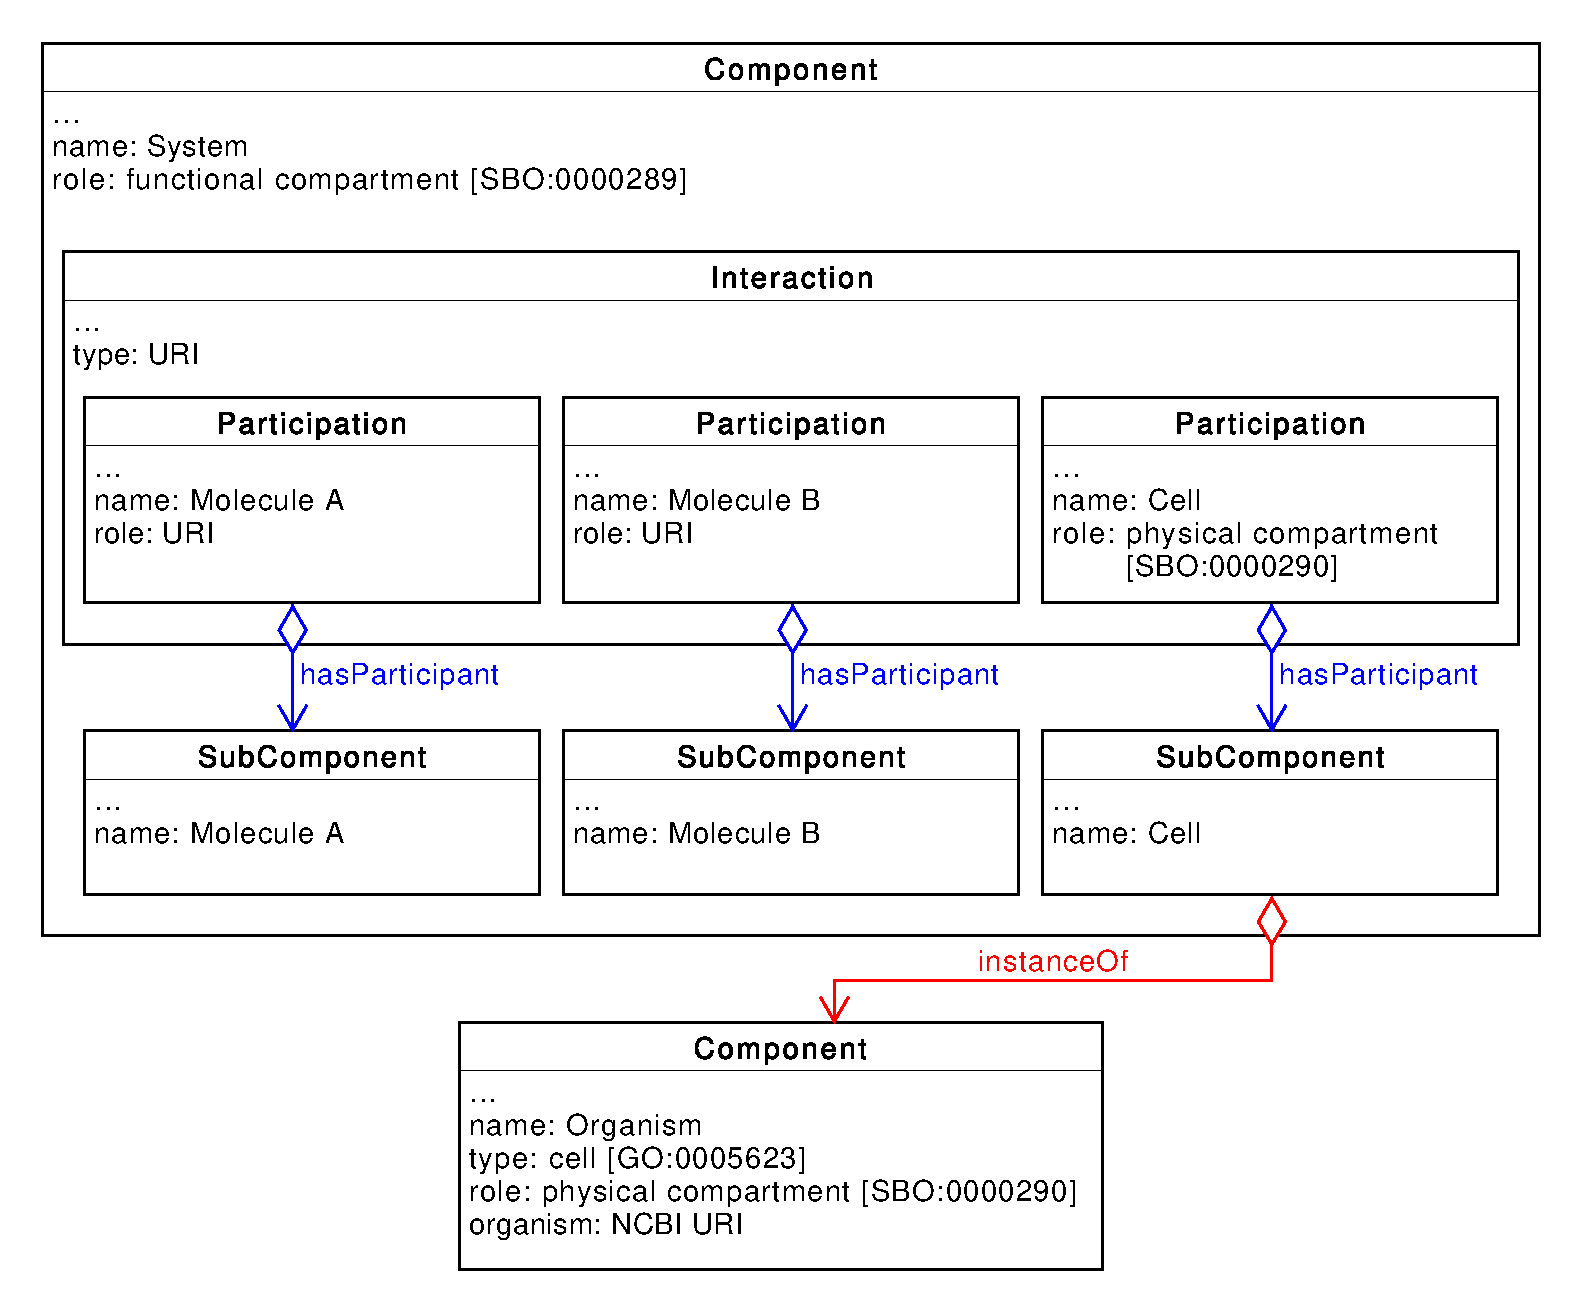
\includegraphics[width=\textwidth]{uml/cell_representation}
		\caption[Repressenting a cell]{This is a proposed approach for capturing cell designs in SBOL. A \sbol{Component} annotated with a URI pointing to an entry in the NCBI Taxonomy Database is used to capture information about the cell's strain/species. 
		The \sbol{Component} has a type of ``Cell'' from the Gene Ontology (GO), and a role of ``physical compartment''. 
		Another \sbol{Component} is used to represent a system in which the cell is implemented. 
		Entities, including the cell, are instantiated as \sbol{SubComponent}s, and processes are captured using the \sbol{Interaction} class.
		Processes that are contained within the cell are represented by including the cell as a participant with a role of ``physical compartment''. }
		\label{uml:cell_representation}
	\end{center}
\end{figure}

\subsubsection{Multiple Cell Types in a Single Design}

The same approach can be extended to represent systems with multiple types of cells.
The multicellular system can be represented as a \sbol{Component} that includes each strain of cell as a \sbol{SubComponent} that is an \sbol{instanceOf} a \sbol{Component} defining its strain.
Interactions and constraints, such as a molecule that both strains interact with, are implemented using \sbol{ComponentReference}s to link to the definitions within each cell system description.
An example is shown in \ref{uml:multiple_cell_representation}.

\begin{figure}[htp]
	\begin{center}
		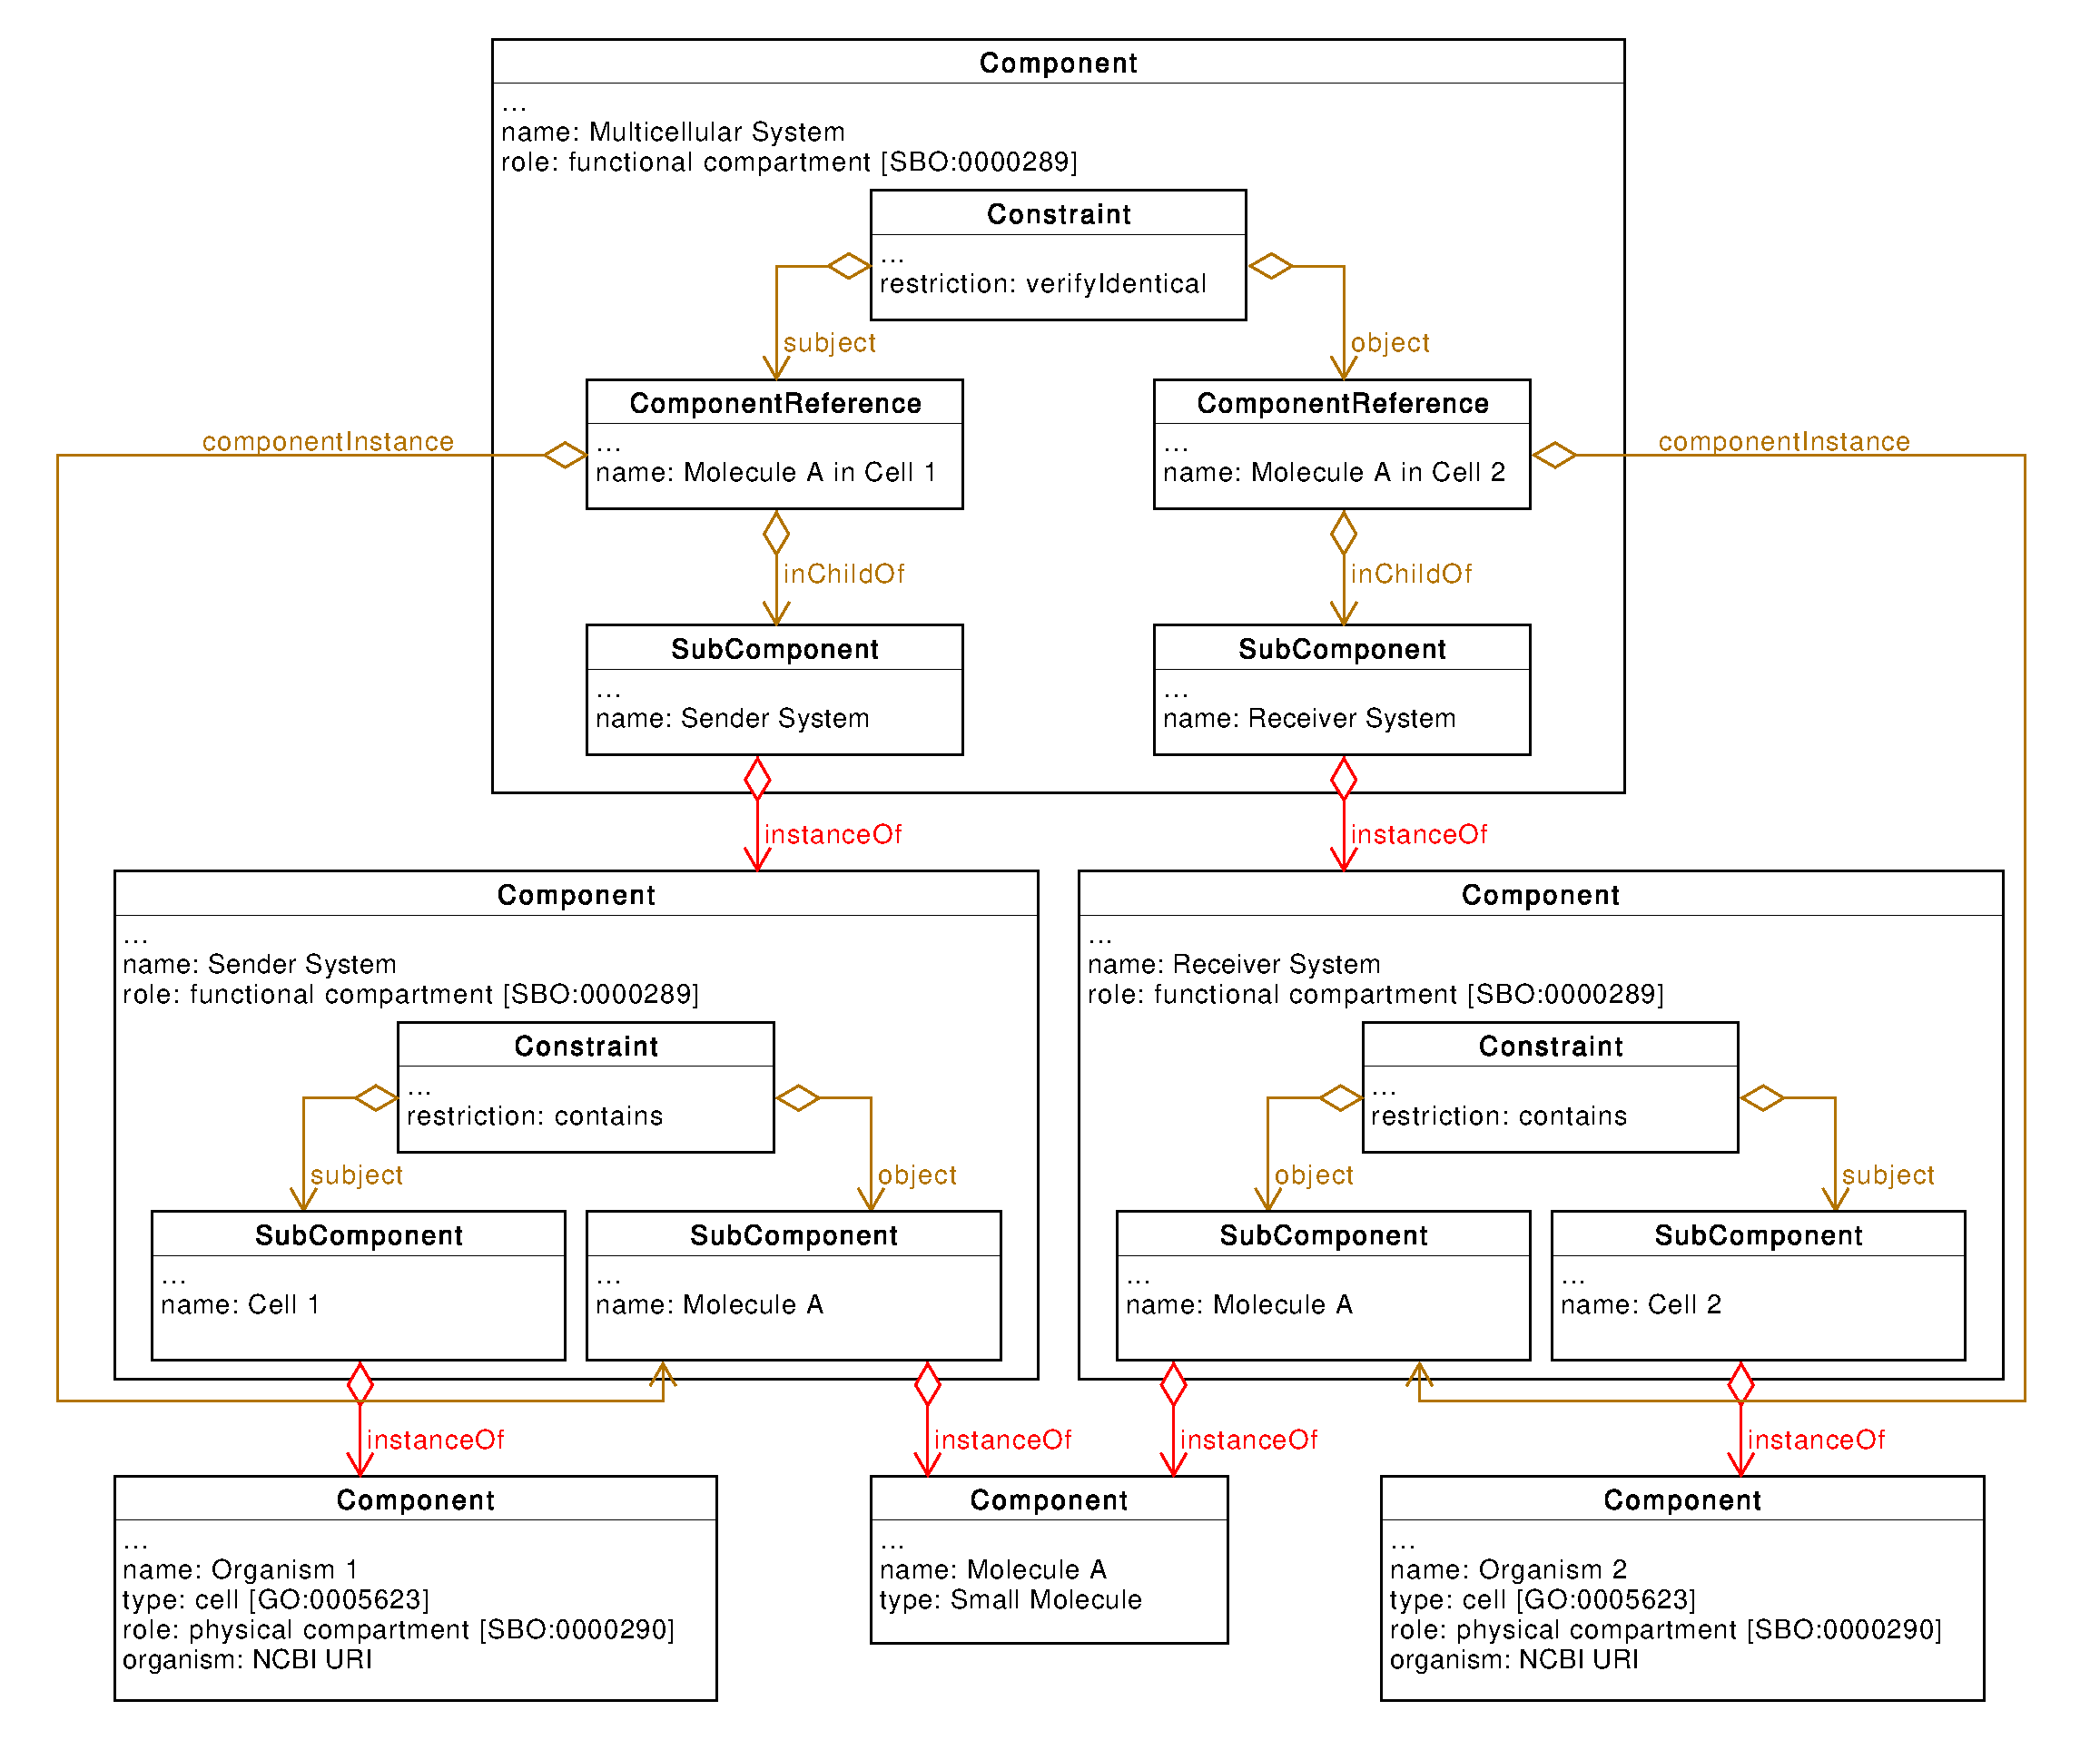
\includegraphics[width=\textwidth]{uml/two_cell_representation}
		\caption[]{Captured here is a design involving two cells which both interact with the small molecule ``Molecule A''. 
		Designs for the sender and receiver systems are captured using constraint to show that each of these cells interacts with the Molecule A contained within it.
		The overall multicellular system is represented by a \sbol{Component} with a \sbolmult{role:C}{role} of ``functional compartment'', which is an SBO term.
		The two systems are included in this multicellular design as \sbol{SubComponent}s, and the fact that Molecule A is shared between systems is indicated with a constraint.}
		\label{uml:multiple_cell_representation}
	\end{center}
\end{figure}

\subsubsection{Cell Ratios}

The proportion of cell types present in a multicellular system can be captured using \om{Measure} on the representations of cells in the design.
As a best practice, the value of these measure classes is a percentage less than or equal to 100\%, representing the amount of a cell type present in the system compared to all other cell types present. 
Therefore, the sum of all these values specified in the system will typically be equal to 100\%, though this may not be the case if the system is not completely defined. 
An example is shown in \ref{uml:cell_ratios}.

\begin{figure}[htp]
	\begin{center}
		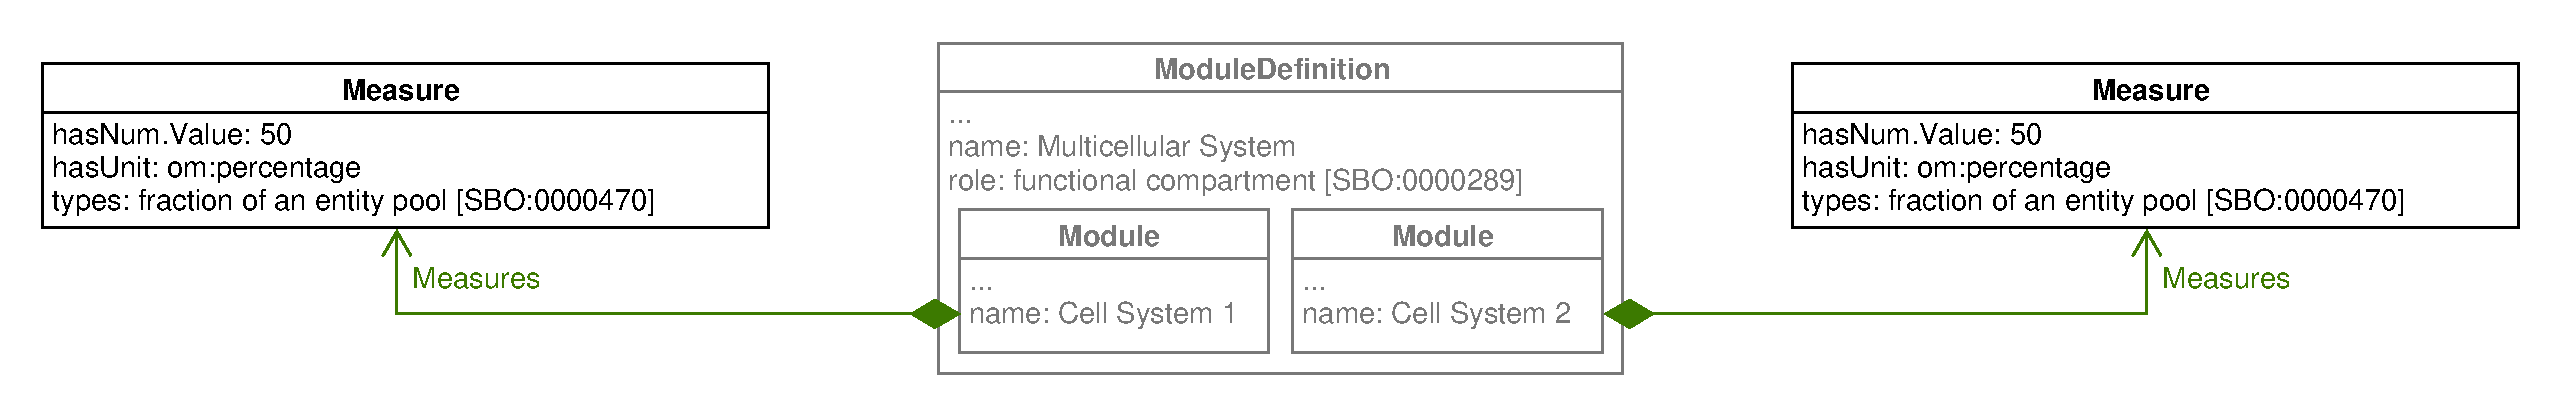
\includegraphics[width=\textwidth]{uml/cell_ratios}
		\caption[]{Annotating class instances with cellular proportions. Instances of the Measure class are used to capture the percentage of each cell type present in the multicellular system design.
		}
		\label{uml:cell_ratios}
	\end{center}
\end{figure}


\newpage
\bibliography{sbol}

\appendix

\newcounter{sbolCtr}
\newcommand{\printValid}{\validRule{sbol-\arabic{sbolCtr}\addtocounter{sbolCtr}{1}}}
\newcommand{\printWarning}{\consistencyRule{sbol-\arabic{sbolCtr}\addtocounter{sbolCtr}{1}}}
\newcommand{\printModeling}{\modelingRule{sbol-\arabic{sbolCtr}\addtocounter{sbolCtr}{1}}}

\section{Validation Rules}
\label{validation}

This section summarizes all the conditions that MUST be or 
are RECOMMENDED to be true of an SBOL Version~2 document.  
There are different degrees of rule strictness.  
Rules of the former kind are strict SBOL validation rules---data encoded in SBOL MUST conform to
all of them in order to be considered valid.  Rules of the latter kind
are consistency rules that are RECCOMENDED for following best practices.  To help highlight these differences, we use the
following symbols next to the rule numbers:

\begin{description}

\item[\hspace*{6.5pt}\vSymbol\vsp] A \vSymbolName indicates a strong
  REQUIRED condition for SBOL conformance. If a SBOL document does not follow this rule, it does not conform to the SBOL
  specification.  (Mnemonic intention behind the choice of symbol:
  ``This must be checked.'')

\item[\hspace*{6.5pt}\cSymbol\csp] A \cSymbolName indicates a weak
  REQUIRED condition for SBOL conformance. While this rule MUST be followed, it is difficult, if not  impossible, for a machine to automatically check whether the rule has been followed. (Mnemonic intention behind the choice of symbol: ``This is a cause for warning.'')

\item[\hspace*{6.5pt}\mSymbol\msp] A \mSymbolName indicates a 
  RECOMMENDED condition for following best practices.  This rule is not strictly a matter of SBOL conformance, but its recommendation comes from logical
  reasoning.  If an SBOL document does not follow this rule, it is still valid SBOL, but it may have degraded functionality in some tools.  (Mnemonic intention behind the choice of symbol: ``You're a star if you heed this.'')

\end{description}

The validation rules listed in the following subsections should all be
stated or implied in the rest of this specification document.  They
are enumerated here for convenience and to provide a ``master
checklist'' for SBOL compliance.  In case of a conflict between this
section and other portions of the specification (though there should
be none), this section is considered authoritative for purpose of
determining SBOL document compliance.

For \notice convenience and brievity, we use the shorthand
``\token{sbol:x}'' to stand for an attribute or element name \token{x}
in the namespace for the SBOL specification, using
the namespace prefix \token{sbol}.  In reality, the prefix string may be different from the literal ``\token{sbol}'' used here (and indeed, it can be any valid XML namespace prefix that the software
chooses).  We use ``\token{sbol:x}'' because it is shorter than to
write a full explanation everywhere we refer to an attribute or element
in the SBOL specification namespace.

\subsubsection*{General rules about an SBOL document}
\setcounter{sbolCtr}{10101} 

\printValid{An SBOL document MUST declare the use of the following XML namespace: \\ \textls[-25]{\uri{http://sbols.org/v2\#}}.\\
Reference: \sec{xml-namespace}}

\printValid{An SBOL document MUST declare the use of the following XML namespace: \\ \textls[-25]{\uri{http://www.w3.org/1999/02/22-rdf-syntax-ns\#}}.\\
Reference: \sec{xml-namespace}}

\printValid{An SBOL document MUST declare the use of the following XML namespace when it includes any \sbol{name} or \sbol{description} properties: \\ \textls[-25]{\uri{http://purl.org/dc/terms/}}.\\ 
Reference: \sec{xml-namespace}}

\printValid{An SBOL document MUST declare the use of the following XML namespace when it includes any \sbol{wasDerivedFrom} properties: \\ \textls[-25]{\uri{http://www.w3.org/ns/prov\#}}.\\ Reference: \sec{xml-namespace}}

\subsubsection*{Rules for the \class{Identified} class} 
\setcounter{sbolCtr}{10201}

\printValid{The \sbol{identity} is a REQUIRED property for all \sbol{Identified} objects and has a data type of URI with a syntax defined by:\\
\uri{http://www.w3.org/1999/02/22-rdf-syntax\#about} \\ 
Reference: \sec{sec:Identified}}

\printValid{The \sbol{persistentIdentity} is an OPTIONAL property for all \sbol{Identified} objects and, if provided, has a data type of \sbol{URI} with a syntax defined by:\\ \uri{http://www.w3.org/1999/02/22-rdf-syntax\#about}\\ 
Reference: \sec{sec:Identified}}

\printValid{The \sbol{displayId} is an OPTIONAL property for all \sbol{Identified} objects and, if provided, has a data type of String that is composed only of alphanumeric or underscore characters and MUST NOT begin with a digit.\\ Reference: \sec{sec:Identified}}

\printValid{The \sbol{version} is an OPTIONAL property for all \sbol{Identified} objects and, if provided, has a data type of String that is composed only of alphanumeric characters, underscores, hyphens, and periods and MUST begin with a digit.\\ Reference: \sec{sec:Identified}}

\printValid{The \sbol{annotations} field is an OPTIONAL list of for all \sbol{Identified} objects and, if provided, includes references to \sbol{Annotation} objects.\\ Reference: \sec{sec:Identified}}

\printValid{The \sbol{wasDerivedFrom} property is OPTIONAL for all \sbol{Identified} objects and, if provided, has a data type of \sbol{URI}.  \\ Reference: \sec{sec:Identified}}

\printValid{The \sbol{name} is an OPTIONAL property for all \sbol{Identified} objects and, if provided, has a data type of String.  \\ Reference: \sec{sec:Identified}}

\printValid{The \sbol{description} is an OPTIONAL property for all \sbol{Identified} objects and, if provided, has a data type of String.  \\ Reference: \sec{sec:Identified}}

\printModeling{The \sbol{displayId} of a compliant object is REQUIRED.  \\ Reference: \sec{sec:compliant}}

\printModeling{The \sbol{persistentIdentity} of a compliant top level object is REQUIRED and MUST end with a delimiter ('/', '\#', or ':') followed by the \sbol{displayId} of the object.\\ Reference: \sec{sec:compliant}}

\printModeling{The \sbol{persistentIdentity} of a compliant child object is REQUIRED and MUST begin with the\\ \sbol{persistentIdentity} of its parent object and be immediately followed by a delimiter ('/', '\#', or ':') and the \sbol{displayId} of the object.\\ Reference: \sec{sec:compliant}}

\printModeling{The \sbol{identity} of a compliant object MUST either be equal to the \sbol{persistentIdentity} when no \sbol{version} is specified or equal to "\refObj{persistentIdentity}/\refObj{version}" when a \sbol{version} is provided.\\ Reference: \sec{sec:compliant}}

\printModeling{The \sbol{version} of a compliant child object is REQUIRED to be equal to the \sbol{version} of its parent object.\\ Reference: \sec{sec:compliant}}

\subsubsection*{Rules for the \class{TopLevel} class} 
\setcounter{sbolCtr}{10301}

\printValid{A \sbol{TopLevel} object inherits all properties of a \sbol{Identified} object.\\ Reference: \sec{sec:TopLevel}}

\subsubsection*{Rules for the \class{Sequence} class} 
\setcounter{sbolCtr}{10401}

\printValid{A \sbol{Sequence} MUST inherit all properties of the \sbol{TopLevel} class.\\ Reference: \sec{sec:Sequence}}

\printValid{The \sbol{elements} property of a \sbol{Sequence} is REQUIRED and MUST contain a \external{String}.\\ Reference: \sec{sec:Sequence}}

\printValid{The \sbol{encoding} property of \sbol{Sequence} is REQUIRED and MUST contain a \external{URI}.\\ Reference: \sec{sec:Sequence}}

\printWarning{The \sbol{encoding} property of a \sbol{Sequence} MUST contain a \external{URI} from \ref{tbl:sequence_encodings} if it is well-described by this \external{URI}.\\ Reference: \sec{sec:Sequence}}

\printWarning{The \sbol{elements} property of a \sbol{Sequence} MUST be consistent with its \sbol{encoding} property.\\ Reference: \sec{sec:Sequence}}

\subsubsection*{Rules for the \class{ComponentDefinition} class} 
\setcounter{sbolCtr}{10501}

\printValid{A \sbol{ComponentDefinition} MUST inherit all properties of the \sbol{TopLevel} class.\\ Reference: \sec{sec:ComponentDefinition}}

\printValid{The \sbolmult{types:CD}{types} property of a \sbol{ComponentDefinition} is REQUIRED and MUST contain a non-empty set of \external{URI}s.\\ Reference: \sec{sec:ComponentDefinition}}

\printValid{The \sbolmult{types:CD}{types} property of a \sbol{ComponentDefinition} MUST NOT contain more than one \external{URI} from \ref{tbl:componentdefinition_types}.\\ Reference: \sec{sec:ComponentDefinition}}

\printWarning{The \sbolmult{types:CD}{types} property of a \sbol{ComponentDefinition} MUST contain a \external{URI} from \ref{tbl:componentdefinition_types} if it is well-described by this \external{URI}.\\ Reference: \sec{sec:ComponentDefinition}}

\printWarning{Each \external{URI} contained by the \sbolmult{types:CD}{types} property of a \sbol{ComponentDefinition} MUST refer to an ontology term that describes the category of biochemical or physical entity that is represented by the \sbol{ComponentDefinition}.\\ Reference: \sec{sec:ComponentDefinition}}

\printWarning{All \external{URI}s contained by the \sbolmult{types:CD}{types} property of a \sbol{ComponentDefinition} MUST refer to non-conflicting ontology terms.\\ Reference: \sec{sec:ComponentDefinition}}

\printValid{The \sbolmult{roles:CD}{roles} property of a \sbol{ComponentDefinition} is OPTIONAL and MAY contain a set of \external{URI}s.\\ Reference: \sec{sec:ComponentDefinition}}

\printWarning{The \sbolmult{roles:CD}{roles} property of a \sbol{ComponentDefinition} MUST contain a \external{URI} from \ref{tbl:componentdefinition_roles} if it is well-described by this \external{URI}.\\ Reference: \sec{sec:ComponentDefinition}}

\printWarning{Each \external{URI} contained by the \sbolmult{roles:CD}{roles} property of a \sbol{ComponentDefinition} MUST refer to an ontology term that clarifies the potential function of the \sbol{ComponentDefinition} in a biochemical or physical context.\\ Reference: \sec{sec:ComponentDefinition}}

\printWarning{Each \external{URI} contained by the \sbolmult{roles:CD}{roles} property of a \sbol{ComponentDefinition} MUST refer to an ontology term that is consistent with its \sbolmult{types:CD}{types} property.\\ Reference: \sec{sec:ComponentDefinition}}

\printModeling{The \sbolmult{roles:CD}{roles} property of a  \sbol{ComponentDefinition} SHOULD only contain a \external{URI} provided in  \ref{tbl:componentdefinition_roles} if one of its \sbolmult{types:CD}{types} is cross-listed with the \external{URI}.\\ Reference: \sec{sec:ComponentDefinition}}

\printValid{The \sbol{sequences} property of a \sbol{ComponentDefinition} is OPTIONAL and MAY contain a set of \external{URI} references to \sbol{Sequence} objects.\\ Reference: \sec{sec:ComponentDefinition}}

\printWarning{Each \external{URI} in the set of \sbol{sequences} MUST reference a \sbol{Sequence} object.\\ Reference: \sec{sec:ComponentDefinition}}

\printWarning{The \sbol{sequences} property of a \sbol{ComponentDefinition} MUST NOT refer to \sbol{Sequence} objects with conflicting \sbol{encoding} properties.\\ Reference: \sec{sec:ComponentDefinition}}

\printWarning{The \sbol{Sequence} objects referred to by the \sbol{sequences} property of a \sbol{ComponentDefinition} MUST be consistent with each other, such that well-defined mappings exist between their \sbol{elements} properties in accordance with their \sbol{encoding} properties.\\ Reference: \sec{sec:ComponentDefinition}}

\printWarning{The \sbol{sequences} property of a \sbol{ComponentDefinition} MUST NOT refer to \sbol{Sequence} objects with conflicting \external{IUPAC} \sbol{encoding} \external{URI}s from \ref{tbl:sequence_encodings}.\\ Reference: \sec{sec:ComponentDefinition}}

\printWarning{If the \sbol{sequences} property of a \sbol{ComponentDefinition} refers to one or more \sbol{Sequence} objects, and one of the  \sbolmult{types:CD}{types} of this \sbol{ComponentDefinition} comes from \ref{tbl:componentdefinition_types}, then one of the \sbol{Sequence} objects MUST have the \sbol{encoding} that is cross-listed with this type in \ref{tbl:sequence_encodings}.\\ Reference: \sec{sec:ComponentDefinition}}

\printWarning{If the \sbol{sequences} property of a \sbol{ComponentDefinition} refers to a \sbol{Sequence} with an \sbol{encoding} from \ref{tbl:sequence_encodings}, then the \sbolmult{types:CD}{types} property of the \sbol{ComponentDefinition} MUST contain the type from \ref{tbl:componentdefinition_types} that is cross-listed with this \sbol{encoding} in  \ref{tbl:sequence_encodings}.\\ Reference: \sec{sec:ComponentDefinition}}

\printModeling{If a \sbol{ComponentDefinition} refers to more than one \sbol{Sequence} with the same \sbol{encoding}, then the \sbol{elements} of these \sbol{Sequence} objects SHOULD have equal lengths.\\ Reference: \sec{sec:ComponentDefinition}}

\printValid{The \sbol{components} property of a \sbol{ComponentDefinition} is OPTIONAL and MAY contain a set of \sbol{Component} objects.\\ Reference: \sec{sec:ComponentDefinition}}

\printModeling{If a \sbol{ComponentDefinition} in a \sbol{ComponentDefinition}-\sbol{Component} hierarchy refers to one or more \sbol{Sequence} objects, and there exist \sbol{ComponentDefinition} objects lower in the hierarchy that refer to \sbol{Sequence} objects with the same \sbol{encoding}, then the \sbol{elements} properties of these \sbol{Sequence} objects SHOULD be consistent with each other, such that well-defined mappings exist from the ``lower level'' \sbol{elements} to the ``higher level'' \sbol{elements} in accordance with their shared \sbol{encoding} (subject to any restrictions on the positions of \sbol{Component} objects in the hierarchy that are imposed by \sbol{SequenceAnnotation} or \sbol{SequenceConstraint} objects).\\ Reference: \sec{sec:ComponentDefinition}}

\printValid{The \sbol{sequenceAnnotations} property of a \sbol{ComponentDefinition} is OPTIONAL and MAY contain a set of \sbol{SequenceAnnotation} objects.\\ Reference: \sec{sec:ComponentDefinition}}

\printValid{If the \sbol{sequenceAnnotations} property of a \sbol{ComponentDefinition} must not contain two or more \sbol{SequenceAnnotation} objects that refer to the same \sbol{Component}.\\ Reference: \sec{sec:ComponentDefinition}}

\printModeling{If the \sbol{sequences} property of a \sbol{ComponentDefinition} refers to a \sbol{Sequence} with an \external{IUPAC} \sbol{encoding} from \ref{tbl:sequence_encodings}, then each \sbol{SequenceAnnotation} that includes a \sbol{Range} and/or \sbol{Cut} in the \sbol{sequenceAnnotations} property of the \sbol{ComponentDefinition} SHOULD specify a region on the \sbol{elements} of this \sbol{Sequence}.\\ Reference: \sec{sec:ComponentDefinition}}

\printValid{The \sbol{sequenceConstraints} property of a \sbol{ComponentDefinition} is OPTIONAL and MAY contain a set of \sbol{SequenceConstraint} objects.  \\ Reference: \sec{sec:ComponentDefinition}}

\subsubsection*{Rules for the \class{ComponentInstance} class} 
\setcounter{sbolCtr}{10601}

\printValid{A \sbol{ComponentInstance} MUST inherit all properties of the \sbol{Identified} class.\\ Reference: \sec{sec:ComponentInstance}}

\printValid{The \sbol{access} property of a \sbol{ComponentInstance} is REQUIRED and MUST contain a \external{URI} from \ref{tbl:componentInstance_access} \\ Reference: \sec{sec:ComponentInstance}}

\printValid{The \sbolmult{definition:CI}{definition} property of a \sbol{ComponentInstance} is REQUIRED and MUST contain a \external{URI} reference to a \sbol{ComponentDefinition}.\\ Reference: \sec{sec:ComponentInstance}}

\printWarning{The \sbol{definition} property \external{URI} must reference a \sbol{ComponentDefinition} object.\\ Reference: \sec{sec:ComponentInstance}}

\printValid{The \sbolmult{definition:CI}{definition} property of a \sbol{ComponentInstance} MUST NOT contain a \external{URI} reference to the \sbol{ComponentDefinition} that contains the \sbol{ComponentInstance}.\\ Reference: \sec{sec:ComponentInstance}}

\printWarning{\sbol{ComponentInstance} objects MUST NOT form circular reference chains via their \sbolmult{definition:CI}{definition} properties and parent \sbol{ComponentDefinition} objects.\\ Reference: \sec{sec:ComponentInstance}}

\printValid{The \sbolmult{mapsTos:CI}{mapsTos} property of a \sbol{ComponentInstance} is OPTIONAL and MAY contain a set of \sbol{MapsTo} objects.\\ Reference: \sec{sec:ComponentInstance}}

\subsubsection*{Rules for the \class{Component} class} 
\setcounter{sbolCtr}{10701}

\printValid{A \sbol{Component} MUST inherit all properties of the \sbol{ComponentInstance} class.\\ Reference: \sec{sec:ComponentInstance}}

\subsubsection*{Rules for the \class{MapsTo} class} 
\setcounter{sbolCtr}{10801}

\printValid{A \sbol{MapsTo} MUST inherit all properties of the \sbol{Identified} class.\\ Reference: \sec{sec:MapsTo}}

\printValid{The \sbol{local} property of a \sbol{MapsTo} is REQUIRED and MUST contain a \external{URI} reference to a \sbol{ComponentInstance}.\\ Reference: \sec{sec:MapsTo}}

\printValid{If a \sbol{MapsTo} is contained by a \sbol{Component} in a \sbol{ComponentDefinition}, then the \sbol{local} property of the \sbol{MapsTo} MUST refer to another \sbol{Component} in the \sbol{ComponentDefinition}.\\ Reference: \sec{sec:MapsTo}}

\printValid{If a \sbol{MapsTo} is contained by a \sbol{FunctionalComponent} or \sbol{Module} in a \sbol{ModuleDefinition}, then the \sbol{local} property of the \sbol{MapsTo} MUST refer to another \sbol{FunctionalComponent} in the \sbol{ModuleDefinition}.\\ Reference: \sec{sec:MapsTo}}

\printValid{The \sbol{remote} property of a \sbol{MapsTo} is REQUIRED and MUST contain a \external{URI} reference to a \sbol{ComponentInstance}.\\ Reference: \sec{sec:MapsTo}}

\printWarning{The \sbol{remote} property of a \sbol{MapsTo} MUST refer to a \sbol{ComponentInstance} with an \sbol{access} property that contains the \external{URI} \url{http://sbols.org/v2\#public}.\\ Reference: \sec{sec:MapsTo}}

\printWarning{If a \sbol{MapsTo} is contained by a \sbol{ComponentInstance}, then the \sbol{remote} property of the \sbol{MapsTo} MUST refer to a \sbol{Component} in the \sbol{ComponentDefinition} that is referenced by the \sbolmult{definition:CI}{definition} of the \sbol{ComponentInstance}.\\ Reference: \sec{sec:MapsTo}} 

\printWarning{If a \sbol{MapsTo} is contained by a \sbol{Module}, then the \sbol{remote} property of the \sbol{MapsTo} MUST refer to a \sbol{FunctionalComponent} in the \sbol{ModuleDefinition} that is referenced by the \sbolmult{definition:CI}{definition} of the \sbol{Module}.\\ Reference: \sec{sec:MapsTo}} 

\printValid{The \sbol{refinement} property is REQUIRED and MUST contain a \external{URI} from \ref{tbl:mapsto_refinement}.
\\ Reference: \sec{sec:MapsTo}}

\subsubsection*{Rules for the \class{SequenceAnnotation} class} 
\setcounter{sbolCtr}{10901}

\printValid{A \sbol{SequenceAnnotation} MUST inherit all properties of the \sbol{Identified} class.\\ Reference: \sec{sec:SequenceAnnotation}}

\printValid{The \sbol{locations} property of a \sbol{SequenceAnnotation} is REQUIRED and MUST contain a non-empty set of \sbol{Location} objects.\\ Reference: \sec{sec:SequenceAnnotation}}

\printWarning{Each \sbol{Location} object in the list of \sbol{locations} should reference a valid location on the corresponding \sbol{Sequence} within the \sbol{ComponentDefinition} (for DNA/RNA/Protein types) that contains the \sbol{SequenceAnnotation}.}

\printValid{The \sbol{component} property is OPTIONAL and MAY contain a \sbol{URI} reference to a \sbol{Component}.\\ Reference: \sec{sec:SequenceAnnotation}}

\printValid{The \sbol{Component} referenced by the \sbol{component} property of a \sbol{SequenceAnnotation} MUST be contained by the \sbol{ComponentDefinition} that contains the \sbol{SequenceAnnotation}.\\ Reference: \sec{sec:SequenceAnnotation}}

\subsubsection*{Rules for the \class{Location} class} 
\setcounter{sbolCtr}{11001}

\printValid{A \sbol{Location} MUST inherit all properties of the \sbol{Identified} class.\\ Reference: \sec{sec:Location}}

\printValid{The \sbol{orientation} property of a \sbol{Location} is OPTIONAL and MAY contain a \sbol{URI} from \ref{tbl:orientation_types}.
\\ Reference: \sec{sec:GenericLocation}}

\subsubsection*{Rules for the \class{Range} class} 
\setcounter{sbolCtr}{11101}

\printValid{A \sbol{Range} MUST inherit all properties of the \sbol{Location} class.\\ Reference: \sec{sec:Range}}

\printValid{The \sbol{start} property of a \sbol{Range} is REQUIRED and MUST contain an \external{Integer} greater than zero.\\ Reference: \sec{sec:Range}}

\printValid{The \sbol{end} property of a \sbol{Range} is REQUIRED and MUST contain an \external{Integer} greater than zero.\\ Reference: \sec{sec:Range}}

\printValid{The value of the \sbol{end} property of a \sbol{Range} MUST be greater than or equal to the value of its \sbol{start} property.\\ Reference: \sec{sec:Range}}


\subsubsection*{Rules for the \class{Cut} class} 
\setcounter{sbolCtr}{11201}

\printValid{A \sbol{Cut} MUST inherit all properties of the \sbol{Location} class.\\ Reference: \sec{sec:Cut}}

\printValid{The \sbol{at} property is REQUIRED and MUST contain an \external{Integer} greater than or equal to zero.  \\ Reference: \sec{sec:Cut}}

\subsubsection*{Rules for the \class{GenericLocation} class} 
\setcounter{sbolCtr}{11301}

\printValid{A \sbol{GenericLocation} MUST inherit all properties of the \sbol{Location} class.\\ Reference: \sec{sec:GenericLocation}}

\subsubsection*{Rules for the \class{SequenceConstraint} class} 
\setcounter{sbolCtr}{11401}

\printValid{A \sbol{SequenceConstraint} MUST inherit all properties of the \sbol{Identified} class.\\ Reference: \sec{sec:SequenceConstraint}}

\printValid{The \sbol{subject} property is REQUIRED and MUST contain a \sbol{URI} reference to a \sbol{Component}.\\ Reference: \sec{sec:SequenceConstraint}}

\printValid{The \sbol{Component} referenced by the \sbol{subject} property of a \sbol{SequenceConstraint} MUST be contained by the \sbol{ComponentDefinition} that contains the \sbol{SequenceConstraint}.\\ Reference: \sec{sec:SequenceConstraint}}

\printValid{The \sbol{object} property is REQUIRED and MUST contain a \sbol{URI} reference to a \sbol{Component}.\\ Reference: \sec{sec:SequenceConstraint}}

\printValid{The \sbol{Component} referenced by the \sbol{object} property of a \sbol{SequenceConstraint} MUST be contained by the \sbol{ComponentDefinition} that contains the \sbol{SequenceConstraint}.\\ Reference: \sec{sec:SequenceConstraint}}

\printValid{The \sbol{object} property of a \sbol{SequenceConstraint} MUST NOT refer to the same \sbol{Component} as the \sbol{subject} property of the \sbol{SequenceConstraint}.\\ Reference: \sec{sec:SequenceConstraint}}

\printValid{The \sbol{restriction} property is REQUIRED and MUST contain a \sbol{URI}.
\\ Reference: \sec{sec:SequenceConstraint}}

\printModeling{The \sbol{URI} contained by the \sbol{restriction} property SHOULD come from \ref{tbl:restriction_types}.
\\ Reference: \sec{sec:SequenceConstraint}}

\subsubsection*{Rules for the \class{Model} class} 
\setcounter{sbolCtr}{11501}

\printValid{A \sbol{Model} object inherits all properties of a \sbol{TopLevel} object.\\ Reference: \sec{sec:Model}}

\printValid{The \sbol{source} property is a REQUIRED \sbol{URI} that specifies the location of the model source file.\\ Reference: \sec{sec:Model}}

\printValid{The \sbol{language} property is a REQUIRED \sbol{URI} that specifies the language in which the model is encoded.\\ Reference: \sec{sec:Model}}

\printModeling{The \sbol{language} property SHOULD be a \sbol{URI} from the EMBRACE Data and Methods (EDAM) ontology.\\ Reference: \sec{sec:Model}}

\printValid{The \sbol{framework} property is a REQUIRED \sbol{URI} that specifies the modeling framework.\\ Reference: \sec{sec:Model}}

\printModeling{The \sbol{framework} property SHOULD be a \sbol{URI} from the  modeling framework branch of the SBO.\\ Reference: \sec{sec:Model}}

\printWarning{The \sbol{source} property MUST specify the location of the model source file in the specified \sbol{language} using the specified \sbol{framework}.\\ Reference: \sec{sec:Model}}

\subsubsection*{Rules for the \class{ModuleDefinition} class} 
\setcounter{sbolCtr}{11601}

\printValid{A \sbol{ModuleDefinition} object inherits all properties of a \sbol{TopLevel} object.\\ Reference: \sec{sec:ModuleDefinition}}

\printValid{The \sbolmult{roles:MD}{roles} property is an OPTIONAL set of \sbol{URI}s.  \\ Reference: \sec{sec:ModuleDefinition}}

\printValid{The \sbol{modules} property is an OPTIONAL set of \sbol{Module} objects.  \\ Reference: \sec{sec:ModuleDefinition}}

\printValid{The \sbol{interactions} property is an OPTIONAL set of \sbol{Interaction} objects.  \\ Reference: \sec{sec:ModuleDefinition}}

\printValid{The \sbol{functionalComponents} property is an OPTIONAL set of \sbol{FunctionalComponent} objects.  \\ Reference: \sec{sec:ModuleDefinition}}

\printValid{The \sbol{models} property is an OPTIONAL set of \sbol{URI}s that reference \sbol{Model} objects.  \\ Reference: \sec{sec:ModuleDefinition}}

\printModeling{Each \sbol{URI} in the set of \sbol{models} SHOULD reference a \sbol{Model} object.  \\ Reference: \sec{sec:ModuleDefinition}}

\subsubsection*{Rules for the \class{FunctionalComponent} class} 
\setcounter{sbolCtr}{11701}

\printValid{A \sbol{FunctionalComponent} MUST inherit all properties of the \sbol{ComponentInstance} class.\\ Reference: \sec{sec:ComponentInstance}}

\printValid{The \sbol{direction} property of a \sbol{FunctionalComponent} is REQUIRED and MUST contain a \sbol{URI} from \ref{tbl:functionalcomponent_directions}.
\\ Reference: \sec{sec:FunctionalComponent}}

\subsubsection*{Rules for the \class{Module} class} 
\setcounter{sbolCtr}{11801}

\printValid{A \sbol{Module} object inherits all properties of an \sbol{Identified} object.\\ Reference: \sec{sec:Module}}

\printValid{The \sbolmult{definition:M}{definition} property is a REQUIRED \sbol{URI} reference to a \sbol{ModuleDefinition} object.  \\ Reference: \sec{sec:Module}}

\printValid{The \sbolmult{mapsTos:M}{mapsTos} property is an OPTIONAL set of \sbol{MapsTo} objects.  \\ Reference: \sec{sec:Module}}

\subsubsection*{Rules for the \class{Interaction} class} 
\setcounter{sbolCtr}{11901}

\printValid{An \sbol{Interaction} object inherits all properties of an \sbol{Identified} object.\\ Reference: \sec{sec:Interaction}}

\printValid{The \sbolmult{types:I}{types} property is a set of \sbol{URI}s, and it is REQUIRED to include at least one entry.\\ Reference: \sec{sec:Interaction}}

\printModeling{A least one type in the set of \sbolmult{types:I}{types} SHOULD be a \sbol{URI} from the occurring entity relationship branch of the SBO.\\ Reference: \sec{sec:Interaction}}

\printValid{The \sbol{participations} property is an OPTIONAL set of \sbol{Participation} objects.\\ Reference: \sec{sec:Interaction}}

\subsubsection*{Rules for the \class{Participation} class} 
\setcounter{sbolCtr}{12001}

\printValid{A \sbol{Participation} object inherits all properties of an \sbol{Identified} object.\\ Reference: \sec{sec:Participation}}

\printValid{The \sbol{participant} property is a REQUIRED \sbol{URI} that MUST reference a \sbol{FunctionalComponent} that is specified within the same \sbol{ModuleDefinition}.\\ Reference: \sec{sec:Participation}}

\printValid{The \sbolmult{roles:P}{roles} property is an OPTIONAL set of \sbol{URI}s.\\ Reference: \sec{sec:Participation}}

\printModeling{A least one role in the set of \sbolmult{roles:P}{roles} SHOULD be a \sbol{URI} from the participant role branch of the SBO.\\ Reference: \sec{sec:Participation}}

\subsubsection*{Rules for the \class{Collection} class} 
\setcounter{sbolCtr}{12101}

\printValid{A \sbol{Collection} object inherits all properties of a \sbol{TopLevel} object.\\ Reference: \sec{sec:Collection}}

\printValid{The \sbol{members} property is an OPTIONAL set of \sbol{URI}s. that reference \sbol{TopLevel} objects.\\ Reference: \sec{sec:Collection}}

\printModeling{Each \sbol{URI} in the set of \sbol{members} SHOULD reference a \sbol{TopLevel} object.\\ Reference: \sec{sec:Collection}}

\subsubsection*{Rules for the \class{Annotation} class} 
\setcounter{sbolCtr}{12201}

\printValid{The \sbol{name} property is REQUIRED, and it has data type \sbol{QName}.\\ Reference: \sec{sec:Annotations}}

\printValid{The \sbol{value} property is REQUIRED, and it has data type \sbol{AnnotationValue}.\\ Reference: \sec{sec:Annotations}}

\printValid{The \sbol{AnnotationValue} class MUST be of data type \sbol{String}, \sbol{Integer}, \sbol{Double}, \sbol{Boolean}, \sbol{URI}, or \sbol{NestedAnnotations}.\\ Reference: \sec{sec:Annotations}}

\printValid{The \sbol{nestedQName} property is REQUIRED for a \sbol{NestedAnnotations} object, and it has data type \sbol{QName}.  \\ Reference: \sec{sec:Annotations}}

\printValid{The \sbol{nestedURI} property is REQUIRED for a \sbol{NestedAnnotations} object, and it has data type \sbol{URI}.  \\ Reference: \sec{sec:Annotations}}

\printValid{The \sbol{annotations} property is an OPTIONAL set for a \sbol{NestedAnnotations} object, and each member is of data type \sbol{Annotation}.  \\ Reference: \sec{sec:Annotations}}

\subsubsection*{Rules for the \class{GenericTopLevel} class} 
\setcounter{sbolCtr}{12301}

\printValid{A \sbol{GenericTopLevel} object inherits all properties of a \sbol{TopLevel} object.\\ Reference: \sec{sec:GenericTopLevel}}

\printValid{The \sbol{rdfType} property is REQUIRED, and it has data type \sbol{QName}.\\ Reference: \sec{sec:GenericTopLevel}}

% -----------------------------------------------------------------------------
\section{Examples of Serialization}
\label{ser:examples}
% -----------------------------------------------------------------------------

\Ctodo{Mike B: ``DNA sequences run off the page.
Historically, this has often been a problem with long DNA string datatypes that don't permit inline whitespace. They're impossible to print or justify for web presentation without breaking the validity of the document.''}

\subsection{PoPS Receiver}

This example shows the serialization of the PoPS Receiver device designed by Canton and co-workers~\cite{canton-natbio-2008}. 
In particular, this is a \sbol{ComponentDefinition} comprising five other \sbol{Component} objects to construct a detector for the cell-cell signaling molecule 3OC$_6$HSL.
The five components are arranged in a sequence:
first come four components together implement constitutive expression of the LuxR protein, which responds to 3OC$_6$HSL: a constitutive promoter, 5'UTR, coding sequence for LuxR, and terminator.
Finally, after this comes the pLuxR promoter, which is activated in the presence of LuxR and 3OC$_6$HSL.
%
Complete details of the device can be found in the cited paper and also at \url{http://parts.igem.org/Part:BBa_F2620}.

\label{ser:F2620}
\lstsetsbol
\begin{lstlisting}
<?xml version="1.0" ?>
<rdf:RDF xmlns:pr="http://partsregistry.org" xmlns:rdf="http://www.w3.org/1999/02/22-rdf-syntax-ns#" xmlns:dcterms="http://purl.org/dc/terms/" xmlns:prov="http://www.w3.org/ns/prov#" xmlns:sbol="http://sbols.org/v2#">
  <sbol:ComponentDefinition rdf:about="http://partsregistry.org/cd/BBa_B0015">
    <sbol:persistentIdentity rdf:resource="http://partsregistry.org/cd/BBa_B0015"/>
    <sbol:displayId>BBa_B0015</sbol:displayId>
    <dcterms:title>BBa_B0015</dcterms:title>
    <dcterms:description>Double terminator</dcterms:description>
    <sbol:type rdf:resource="http://www.biopax.org/release/biopax-level3.owl#DnaRegion"/>
    <sbol:role rdf:resource="http://identifiers.org/so/SO:0000141"/>
    <sbol:sequence rdf:resource="http://partsregistry.org/seq/BBa_B0015"/>
  </sbol:ComponentDefinition>
  <sbol:ComponentDefinition rdf:about="http://partsregistry.org/cd/BBa_R0062">
    <sbol:persistentIdentity rdf:resource="http://partsregistry.org/cd/BBa_R0062"/>
    <sbol:displayId>BBa_R0062</sbol:displayId>
    <dcterms:title>BBa_R0062</dcterms:title>
    <dcterms:description>LuxR inducible promoter</dcterms:description>
    <sbol:type rdf:resource="http://www.biopax.org/release/biopax-level3.owl#DnaRegion"/>
    <sbol:role rdf:resource="http://identifiers.org/so/SO:0000167"/>
    <sbol:sequence rdf:resource="http://partsregistry.org/seq/BBa_R0062"/>
  </sbol:ComponentDefinition>
  <sbol:ComponentDefinition rdf:about="http://partsregistry.org/cd/BBa_C0062">
    <sbol:persistentIdentity rdf:resource="http://partsregistry.org/cd/BBa_C0062"/>
    <sbol:displayId>BBa_C0062</sbol:displayId>
    <dcterms:title>BBa_C0062</dcterms:title>
    <dcterms:description>luxR coding sequence</dcterms:description>
    <sbol:type rdf:resource="http://www.biopax.org/release/biopax-level3.owl#DnaRegion"/>
    <sbol:role rdf:resource="http://identifiers.org/so/SO:0000316"/>
    <sbol:sequence rdf:resource="http://partsregistry.org/seq/BBa_C0062"/>
  </sbol:ComponentDefinition>
  <sbol:ComponentDefinition rdf:about="http://partsregistry.org/cd/BBa_R0040">
    <sbol:persistentIdentity rdf:resource="http://partsregistry.org/cd/BBa_R0040"/>
    <sbol:displayId>BBa_R0040</sbol:displayId>
    <dcterms:title>BBa_R0040</dcterms:title>
    <dcterms:description>TetR repressible promoter</dcterms:description>
    <sbol:type rdf:resource="http://www.biopax.org/release/biopax-level3.owl#DnaRegion"/>
    <sbol:role rdf:resource="http://identifiers.org/so/SO:0000167"/>
    <sbol:sequence rdf:resource="http://partsregistry.org/seq/BBa_R0040"/>
  </sbol:ComponentDefinition>
  <sbol:ComponentDefinition rdf:about="http://partsregistry.org/cd/BBa_B0034">
    <sbol:persistentIdentity rdf:resource="http://partsregistry.org/cd/BBa_B0034"/>
    <sbol:displayId>BBa_B0034</sbol:displayId>
    <dcterms:title>BBa_B0034</dcterms:title>
    <dcterms:description>RBS based on Elowitz repressilator</dcterms:description>
    <sbol:type rdf:resource="http://www.biopax.org/release/biopax-level3.owl#DnaRegion"/>
    <sbol:role rdf:resource="http://identifiers.org/so/SO:0000139"/>
    <sbol:sequence rdf:resource="http://partsregistry.org/seq/BBa_B0034"/>
  </sbol:ComponentDefinition>
  <sbol:ComponentDefinition rdf:about="http://partsregistry.org/cd/BBa_F2620">
    <sbol:persistentIdentity rdf:resource="http://partsregistry.org/cd/BBa_F2620"/>
    <sbol:displayId>BBa_F2620</sbol:displayId>
    <dcterms:title>BBa_F2620</dcterms:title>
    <dcterms:description>3OC6HSL -&gt; PoPS Receiver</dcterms:description>
    <sbol:type rdf:resource="http://www.biopax.org/release/biopax-level3.owl#DnaRegion"/>
    <sbol:role rdf:resource="http://identifiers.org/so/SO:00001411"/>
    <sbol:component>
      <sbol:Component rdf:about="http://partsregistry.org/cd/BBa_F2620/pLuxR">
        <sbol:persistentIdentity rdf:resource="http://partsregistry.org/cd/BBa_F2620/pLuxR"/>
        <sbol:displayId>pLuxR</sbol:displayId>
        <sbol:access rdf:resource="http://sbols.org/v2#public"/>
        <sbol:definition rdf:resource="http://partsregistry.org/cd/BBa_R0062"/>
      </sbol:Component>
    </sbol:component>
    <sbol:component>
      <sbol:Component rdf:about="http://partsregistry.org/cd/BBa_F2620/luxR">
        <sbol:persistentIdentity rdf:resource="http://partsregistry.org/cd/BBa_F2620/luxR"/>
        <sbol:displayId>luxR</sbol:displayId>
        <sbol:access rdf:resource="http://sbols.org/v2#public"/>
        <sbol:definition rdf:resource="http://partsregistry.org/cd/BBa_B0034"/>
      </sbol:Component>
    </sbol:component>
    <sbol:component>
      <sbol:Component rdf:about="http://partsregistry.org/cd/BBa_F2620/pTetR">
        <sbol:persistentIdentity rdf:resource="http://partsregistry.org/cd/BBa_F2620/pTetR"/>
        <sbol:displayId>pTetR</sbol:displayId>
        <sbol:access rdf:resource="http://sbols.org/v2#public"/>
        <sbol:definition rdf:resource="http://partsregistry.org/cd/BBa_R0040"/>
      </sbol:Component>
    </sbol:component>
    <sbol:component>
      <sbol:Component rdf:about="http://partsregistry.org/cd/BBa_F2620/ter">
        <sbol:persistentIdentity rdf:resource="http://partsregistry.org/cd/BBa_F2620/ter"/>
        <sbol:displayId>ter</sbol:displayId>
        <sbol:access rdf:resource="http://sbols.org/v2#public"/>
        <sbol:definition rdf:resource="http://partsregistry.org/cd/BBa_B0015"/>
      </sbol:Component>
    </sbol:component>
    <sbol:component>
      <sbol:Component rdf:about="http://partsregistry.org/cd/BBa_F2620/rbs">
        <sbol:persistentIdentity rdf:resource="http://partsregistry.org/cd/BBa_F2620/rbs"/>
        <sbol:displayId>rbs</sbol:displayId>
        <sbol:access rdf:resource="http://sbols.org/v2#public"/>
        <sbol:definition rdf:resource="http://partsregistry.org/cd/BBa_C0062"/>
      </sbol:Component>
    </sbol:component>
    <sbol:sequenceAnnotation>
      <sbol:SequenceAnnotation rdf:about="http://partsregistry.org/cd/BBa_F2620/anno3">
        <sbol:persistentIdentity rdf:resource="http://partsregistry.org/cd/BBa_F2620/anno3"/>
        <sbol:displayId>anno3</sbol:displayId>
        <sbol:location>
          <sbol:Range rdf:about="http://partsregistry.org/cd/BBa_F2620/anno3/range">
            <sbol:persistentIdentity rdf:resource="http://partsregistry.org/cd/BBa_F2620/anno3/range"/>
            <sbol:displayId>range</sbol:displayId>
            <sbol:start>69</sbol:start>
            <sbol:end>770</sbol:end>
            <sbol:orientation rdf:resource="http://sbols.org/v2#inline"/>
          </sbol:Range>
        </sbol:location>
        <sbol:component rdf:resource="http://partsregistry.org/cd/BBa_F2620/luxR"/>
      </sbol:SequenceAnnotation>
    </sbol:sequenceAnnotation>
    <sbol:sequenceAnnotation>
      <sbol:SequenceAnnotation rdf:about="http://partsregistry.org/cd/BBa_F2620/anno4">
        <sbol:persistentIdentity rdf:resource="http://partsregistry.org/cd/BBa_F2620/anno4"/>
        <sbol:displayId>anno4</sbol:displayId>
        <sbol:location>
          <sbol:Range rdf:about="http://partsregistry.org/cd/BBa_F2620/anno4/range">
            <sbol:persistentIdentity rdf:resource="http://partsregistry.org/cd/BBa_F2620/anno4/range"/>
            <sbol:displayId>range</sbol:displayId>
            <sbol:start>771</sbol:start>
            <sbol:end>900</sbol:end>
            <sbol:orientation rdf:resource="http://sbols.org/v2#inline"/>
          </sbol:Range>
        </sbol:location>
        <sbol:component rdf:resource="http://partsregistry.org/cd/BBa_F2620/ter"/>
      </sbol:SequenceAnnotation>
    </sbol:sequenceAnnotation>
    <sbol:sequenceAnnotation>
      <sbol:SequenceAnnotation rdf:about="http://partsregistry.org/cd/BBa_F2620/anno1">
        <sbol:persistentIdentity rdf:resource="http://partsregistry.org/cd/BBa_F2620/anno1"/>
        <sbol:displayId>anno1</sbol:displayId>
        <sbol:location>
          <sbol:Range rdf:about="http://partsregistry.org/cd/BBa_F2620/anno1/range">
            <sbol:persistentIdentity rdf:resource="http://partsregistry.org/cd/BBa_F2620/anno1/range"/>
            <sbol:displayId>range</sbol:displayId>
            <sbol:start>1</sbol:start>
            <sbol:end>55</sbol:end>
            <sbol:orientation rdf:resource="http://sbols.org/v2#inline"/>
          </sbol:Range>
        </sbol:location>
        <sbol:component rdf:resource="http://partsregistry.org/cd/BBa_F2620/pTetR"/>
      </sbol:SequenceAnnotation>
    </sbol:sequenceAnnotation>
    <sbol:sequenceAnnotation>
      <sbol:SequenceAnnotation rdf:about="http://partsregistry.org/cd/BBa_F2620/anno5">
        <sbol:persistentIdentity rdf:resource="http://partsregistry.org/cd/BBa_F2620/anno5"/>
        <sbol:displayId>anno5</sbol:displayId>
        <sbol:location>
          <sbol:Range rdf:about="http://partsregistry.org/cd/BBa_F2620/anno5/range">
            <sbol:persistentIdentity rdf:resource="http://partsregistry.org/cd/BBa_F2620/anno5/range"/>
            <sbol:displayId>range</sbol:displayId>
            <sbol:start>901</sbol:start>
            <sbol:end>956</sbol:end>
            <sbol:orientation rdf:resource="http://sbols.org/v2#inline"/>
          </sbol:Range>
        </sbol:location>
        <sbol:component rdf:resource="http://partsregistry.org/cd/BBa_F2620/pLuxR"/>
      </sbol:SequenceAnnotation>
    </sbol:sequenceAnnotation>
    <sbol:sequenceAnnotation>
      <sbol:SequenceAnnotation rdf:about="http://partsregistry.org/cd/BBa_F2620/anno2">
        <sbol:persistentIdentity rdf:resource="http://partsregistry.org/cd/BBa_F2620/anno2"/>
        <sbol:displayId>anno2</sbol:displayId>
        <sbol:location>
          <sbol:Range rdf:about="http://partsregistry.org/cd/BBa_F2620/anno2/range">
            <sbol:persistentIdentity rdf:resource="http://partsregistry.org/cd/BBa_F2620/anno2/range"/>
            <sbol:displayId>range</sbol:displayId>
            <sbol:start>56</sbol:start>
            <sbol:end>68</sbol:end>
            <sbol:orientation rdf:resource="http://sbols.org/v2#inline"/>
          </sbol:Range>
        </sbol:location>
        <sbol:component rdf:resource="http://partsregistry.org/cd/BBa_F2620/rbs"/>
      </sbol:SequenceAnnotation>
    </sbol:sequenceAnnotation>
  </sbol:ComponentDefinition>
  <sbol:Sequence rdf:about="http://partsregistry.org/seq/BBa_B0034">
    <sbol:persistentIdentity rdf:resource="http://partsregistry.org/seq/BBa_B0034"/>
    <sbol:displayId>BBa_B0034</sbol:displayId>
    <sbol:elements>aaagaggagaaa</sbol:elements>
    <sbol:encoding rdf:resource="http://www.chem.qmul.ac.uk/iubmb/misc/naseq.html"/>
  </sbol:Sequence>
  <sbol:Sequence rdf:about="http://partsregistry.org/seq/BBa_R0040">
    <sbol:persistentIdentity rdf:resource="http://partsregistry.org/seq/BBa_R0040"/>
    <sbol:displayId>BBa_R0040</sbol:displayId>
    <sbol:elements>tccctatcagtgatagagattgacatccctatcagtgatagagatactgagcac</sbol:elements>
    <sbol:encoding rdf:resource="http://www.chem.qmul.ac.uk/iubmb/misc/naseq.html"/>
  </sbol:Sequence>
  <sbol:Sequence rdf:about="http://partsregistry.org/seq/BBa_C0062">
    <sbol:persistentIdentity rdf:resource="http://partsregistry.org/seq/BBa_C0062"/>
    <sbol:displayId>BBa_C0062</sbol:displayId>
    <sbol:elements>atgcttatctgatatgactaaaatggtacattgtgaatattatttactcgcgatcatttatcctcattctatggttaaatctgatatttcaatcctagataattaccctaaaaaatggaggcaatattatgatgacgctaatttaataaaatatgatcctatagtagattattctaactccaatcattcaccaattaattggaatatatttgaaaacaatgctgtaaataaaaaatctccaaatgtaattaaagaagcgaaaacatcaggtcttatcactgggtttagtttccctattcatacggctaacaatggcttcggaatgcttagttttgcacattcagaaaaagacaactatatagatagtttatttttacatgcgtgtatgaacataccattaattgttccttctctagttgataattatcgaaaaataaatatagcaaataataaatcaaacaacgatttaaccaaaagagaaaaagaatgtttagcgtgggcatgcgaaggaaaaagctcttgggatatttcaaaaatattaggttgcagtgagcgtactgtcactttccatttaaccaatgcgcaaatgaaactcaatacaacaaaccgctgccaaagtatttctaaagcaattttaacaggagcaattgattgcccatactttaaaaattaataacactgatagtgctagtgtagatcac</sbol:elements>
    <sbol:encoding rdf:resource="http://www.chem.qmul.ac.uk/iubmb/misc/naseq.html"/>
  </sbol:Sequence>
  <sbol:Sequence rdf:about="http://partsregistry.org/seq/BBa_R0062">
    <sbol:persistentIdentity rdf:resource="http://partsregistry.org/seq/BBa_R0062"/>
    <sbol:displayId>BBa_R0062</sbol:displayId>
    <sbol:elements>acctgtaggatcgtacaggtttacgcaagaaaatggtttgttatagtcgaataaa</sbol:elements>
    <sbol:encoding rdf:resource="http://www.chem.qmul.ac.uk/iubmb/misc/naseq.html"/>
  </sbol:Sequence>
  <sbol:Sequence rdf:about="http://partsregistry.org/seq/BBa_B0015">
    <sbol:persistentIdentity rdf:resource="http://partsregistry.org/seq/BBa_B0015"/>
    <sbol:displayId>BBa_B0015</sbol:displayId>
    <sbol:elements>ccaggcatcaaataaaacgaaaggctcagtcgaaagactgggcctttcgttttatctgttgtttgtcggtgaacgctctctactagagtcacactggctcaccttcgggtgggcctttctgcgtttata</sbol:elements>
    <sbol:encoding rdf:resource="http://www.chem.qmul.ac.uk/iubmb/misc/naseq.html"/>
  </sbol:Sequence>
</rdf:RDF>
\end{lstlisting}

\subsection{Toggle Switch}

This example shows the serialization of an SBOL data model for a LacI/TetR toggle switch similar to those constructed in \cite{Gardner2000}.  
This design is essentially similar to the one presented in \ref{sec:examples}, except that it uses some alternate groupings in how the total design is built up out of smaller entities.

\label{ser:toggleswitch}
\lstsetsbol
\begin{lstlisting}
<?xml version="1.0" ?>
<rdf:RDF xmlns:rdf="http://www.w3.org/1999/02/22-rdf-syntax-ns#" xmlns:dcterms="http://purl.org/dc/terms/" xmlns:prov="http://www.w3.org/ns/prov#" xmlns:sbol="http://sbols.org/v2#">
  <sbol:ModuleDefinition rdf:about="http://sbolstandard.org/example/toggle_switch">
    <sbol:persistentIdentity rdf:resource="http://sbolstandard.org/example/toggle_switch"/>
    <sbol:displayId>toggle_switch</sbol:displayId>
    <sbol:role rdf:resource="http://sbolstandard.org/example/module_role/toggle_switch"/>
    <sbol:functionalComponent>
      <sbol:FunctionalComponent rdf:about="http://sbolstandard.org/example/toggle_switch/LacI">
        <sbol:persistentIdentity rdf:resource="http://sbolstandard.org/example/toggle_switch/LacI"/>
        <sbol:displayId>LacI</sbol:displayId>
        <sbol:definition rdf:resource="http://identifiers.org/uniprot/P03023"/>
        <sbol:access rdf:resource="http://sbols.org/v2#public"/>
        <sbol:direction rdf:resource="http://sbols.org/v2#inout"/>
      </sbol:FunctionalComponent>
    </sbol:functionalComponent>
    <sbol:functionalComponent>
      <sbol:FunctionalComponent rdf:about="http://sbolstandard.org/example/toggle_switch/TetR">
        <sbol:persistentIdentity rdf:resource="http://sbolstandard.org/example/toggle_switch/TetR"/>
        <sbol:displayId>TetR</sbol:displayId>
        <sbol:definition rdf:resource="http://identifiers.org/uniprot/Q6QR72"/>
        <sbol:access rdf:resource="http://sbols.org/v2#public"/>
        <sbol:direction rdf:resource="http://sbols.org/v2#inout"/>
      </sbol:FunctionalComponent>
    </sbol:functionalComponent>
    <sbol:model rdf:resource="http://sbolstandard.org/example/toogleswicth"/>
    <sbol:module>
      <sbol:Module rdf:about="http://sbolstandard.org/example/toggle_switch/laci_inverter">
        <sbol:persistentIdentity rdf:resource="http://sbolstandard.org/example/toggle_switch/laci_inverter"/>
        <sbol:displayId>laci_inverter</sbol:displayId>
        <sbol:definition rdf:resource="http://sbolstandard.org/example/laci_inverter"/>
        <sbol:mapsTo>
          <sbol:MapsTo rdf:about="http://sbolstandard.org/example/toggle_switch/laci_inverter/LacI_mapping">
            <sbol:persistentIdentity rdf:resource="http://sbolstandard.org/example/toggle_switch/laci_inverter/LacI_mapping"/>
            <sbol:displayId>LacI_mapping</sbol:displayId>
            <sbol:refinement rdf:resource="http://sbols.org/v2#useRemote"/>
            <sbol:remote rdf:resource="http://sbolstandard.org/example/toggle_switch/LacI"/>
            <sbol:local rdf:resource="http://sbolstandard.org/example/laci_inverter/TF"/>
          </sbol:MapsTo>
        </sbol:mapsTo>
      </sbol:Module>
    </sbol:module>
    <sbol:module>
      <sbol:Module rdf:about="http://sbolstandard.org/example/toggle_switch/tetr_inverter">
        <sbol:persistentIdentity rdf:resource="http://sbolstandard.org/example/toggle_switch/tetr_inverter"/>
        <sbol:displayId>tetr_inverter</sbol:displayId>
        <sbol:definition rdf:resource="http://sbolstandard.org/example/tetr_inverter"/>
        <sbol:mapsTo>
          <sbol:MapsTo rdf:about="http://sbolstandard.org/example/toggle_switch/tetr_inverter/TetR_mapping">
            <sbol:persistentIdentity rdf:resource="http://sbolstandard.org/example/toggle_switch/tetr_inverter/TetR_mapping"/>
            <sbol:displayId>TetR_mapping</sbol:displayId>
            <sbol:refinement rdf:resource="http://sbols.org/v2#useRemote"/>
            <sbol:remote rdf:resource="http://sbolstandard.org/example/toggle_switch/TetR"/>
            <sbol:local rdf:resource="http://sbolstandard.org/example/tetr_inverter/TF"/>
          </sbol:MapsTo>
        </sbol:mapsTo>
      </sbol:Module>
    </sbol:module>
  </sbol:ModuleDefinition>
  <sbol:ModuleDefinition rdf:about="http://sbolstandard.org/example/laci_inverter">
    <sbol:persistentIdentity rdf:resource="http://sbolstandard.org/example/laci_inverter"/>
    <sbol:displayId>laci_inverter</sbol:displayId>
    <sbol:role rdf:resource="http://parts.igem.org/cgi/partsdb/pgroup.cgi?pgroup=inverter"/>
    <sbol:functionalComponent>
      <sbol:FunctionalComponent rdf:about="http://sbolstandard.org/example/laci_inverter/TF">
        <sbol:persistentIdentity rdf:resource="http://sbolstandard.org/example/laci_inverter/TF"/>
        <sbol:displayId>TF</sbol:displayId>
        <sbol:definition rdf:resource="http://identifiers.org/uniprot/P03023"/>
        <sbol:access rdf:resource="http://sbols.org/v2#public"/>
        <sbol:direction rdf:resource="http://sbols.org/v2#inout"/>
      </sbol:FunctionalComponent>
    </sbol:functionalComponent>
    <sbol:functionalComponent>
      <sbol:FunctionalComponent rdf:about="http://sbolstandard.org/example/laci_inverter/promoter">
        <sbol:persistentIdentity rdf:resource="http://sbolstandard.org/example/laci_inverter/promoter"/>
        <sbol:displayId>promoter</sbol:displayId>
        <sbol:definition rdf:resource="http://www.partsregistry.org/BBa_R0010"/>
        <sbol:access rdf:resource="http://sbols.org/v2#public"/>
        <sbol:direction rdf:resource="http://sbols.org/v2#inout"/>
      </sbol:FunctionalComponent>
    </sbol:functionalComponent>
    <sbol:interaction>
      <sbol:Interaction rdf:about="http://sbolstandard.org/example/laci_inverter/LacI_pLacI">
        <sbol:persistentIdentity rdf:resource="http://sbolstandard.org/example/laci_inverter/LacI_pLacI"/>
        <sbol:displayId>LacI_pLacI</sbol:displayId>
        <sbol:type rdf:resource="http://identifiers.org/biomodels.sbo/SBO:0000169"/>
        <sbol:participation>
          <sbol:Participation rdf:about="http://sbolstandard.org/example/laci_inverter/LacI_pLacI/BBa_R0010">
            <sbol:persistentIdentity rdf:resource="http://sbolstandard.org/example/laci_inverter/LacI_pLacI/BBa_R0010"/>
            <sbol:displayId>BBa_R0010</sbol:displayId>
            <sbol:role rdf:resource="http://identifiers.org/biomodels.sbo/SBO:0000598"/>
            <sbol:participant rdf:resource="http://sbolstandard.org/example/laci_inverter/promoter"/>
          </sbol:Participation>
        </sbol:participation>
        <sbol:participation>
          <sbol:Participation rdf:about="http://sbolstandard.org/example/laci_inverter/LacI_pLacI/P03023">
            <sbol:persistentIdentity rdf:resource="http://sbolstandard.org/example/laci_inverter/LacI_pLacI/P03023"/>
            <sbol:displayId>P03023</sbol:displayId>
            <sbol:role rdf:resource="http://identifiers.org/biomodels.sbo/SBO:0000020"/>
            <sbol:participant rdf:resource="http://sbolstandard.org/example/laci_inverter/TF"/>
          </sbol:Participation>
        </sbol:participation>
      </sbol:Interaction>
    </sbol:interaction>
  </sbol:ModuleDefinition>
  <sbol:ModuleDefinition rdf:about="http://sbolstandard.org/example/tetr_inverter">
    <sbol:persistentIdentity rdf:resource="http://sbolstandard.org/example/tetr_inverter"/>
    <sbol:displayId>tetr_inverter</sbol:displayId>
    <sbol:role rdf:resource="http://parts.igem.org/cgi/partsdb/pgroup.cgi?pgroup=inverter"/>
    <sbol:functionalComponent>
      <sbol:FunctionalComponent rdf:about="http://sbolstandard.org/example/tetr_inverter/promoter">
        <sbol:persistentIdentity rdf:resource="http://sbolstandard.org/example/tetr_inverter/promoter"/>
        <sbol:displayId>promoter</sbol:displayId>
        <sbol:definition rdf:resource="http://www.partsregistry.org/BBa_R0040"/>
        <sbol:access rdf:resource="http://sbols.org/v2#public"/>
        <sbol:direction rdf:resource="http://sbols.org/v2#inout"/>
      </sbol:FunctionalComponent>
    </sbol:functionalComponent>
    <sbol:functionalComponent>
      <sbol:FunctionalComponent rdf:about="http://sbolstandard.org/example/tetr_inverter/TF">
        <sbol:persistentIdentity rdf:resource="http://sbolstandard.org/example/tetr_inverter/TF"/>
        <sbol:displayId>TF</sbol:displayId>
        <sbol:definition rdf:resource="http://identifiers.org/uniprot/Q6QR72"/>
        <sbol:access rdf:resource="http://sbols.org/v2#public"/>
        <sbol:direction rdf:resource="http://sbols.org/v2#inout"/>
      </sbol:FunctionalComponent>
    </sbol:functionalComponent>
    <sbol:interaction>
      <sbol:Interaction rdf:about="http://sbolstandard.org/example/tetr_inverter/LacI_pLacI">
        <sbol:persistentIdentity rdf:resource="http://sbolstandard.org/example/tetr_inverter/LacI_pLacI"/>
        <sbol:displayId>LacI_pLacI</sbol:displayId>
        <sbol:type rdf:resource="http://identifiers.org/biomodels.sbo/SBO:0000169"/>
        <sbol:participation>
          <sbol:Participation rdf:about="http://sbolstandard.org/example/tetr_inverter/LacI_pLacI/Q6QR72">
            <sbol:persistentIdentity rdf:resource="http://sbolstandard.org/example/tetr_inverter/LacI_pLacI/Q6QR72"/>
            <sbol:displayId>Q6QR72</sbol:displayId>
            <sbol:role rdf:resource="http://identifiers.org/biomodels.sbo/SBO:0000020"/>
            <sbol:participant rdf:resource="http://sbolstandard.org/example/tetr_inverter/TF"/>
          </sbol:Participation>
        </sbol:participation>
        <sbol:participation>
          <sbol:Participation rdf:about="http://sbolstandard.org/example/tetr_inverter/LacI_pLacI/BBa_R0040">
            <sbol:persistentIdentity rdf:resource="http://sbolstandard.org/example/tetr_inverter/LacI_pLacI/BBa_R0040"/>
            <sbol:displayId>BBa_R0040</sbol:displayId>
            <sbol:role rdf:resource="http://identifiers.org/biomodels.sbo/SBO:0000598"/>
            <sbol:participant rdf:resource="http://sbolstandard.org/example/tetr_inverter/promoter"/>
          </sbol:Participation>
        </sbol:participation>
      </sbol:Interaction>
    </sbol:interaction>
  </sbol:ModuleDefinition>
  <sbol:Model rdf:about="http://sbolstandard.org/example/toogleswicth">
    <sbol:persistentIdentity rdf:resource="http://sbolstandard.org/example/toogleswicth"/>
    <sbol:displayId>toogleswicth</sbol:displayId>
    <sbol:source rdf:resource="http://virtualparts.org/part/pIKE_Toggle_1"/>
    <sbol:language rdf:resource="http://identifiers.org/edam/format_2585"/>
    <sbol:framework rdf:resource="http://identifiers.org/biomodels.sbo/SBO:0000062"/>
  </sbol:Model>
  <sbol:ComponentDefinition rdf:about="http://www.partsregistry.org/BBa_J61130">
    <sbol:persistentIdentity rdf:resource="http://www.partsregistry.org/BBa_J61130"/>
    <sbol:displayId>BBa_J61130</sbol:displayId>
    <dcterms:title>BBa_J61101 RBS</dcterms:title>
    <dcterms:description>RBS2</dcterms:description>
    <sbol:type rdf:resource="http://www.biopax.org/release/biopax-level3.owl#DnaRegion"/>
    <sbol:role rdf:resource="http://identifiers.org/so/SO:0000139"/>
    <sbol:sequence rdf:resource="http://www.virtualparts.org/part/BBa_J61130"/>
  </sbol:ComponentDefinition>
  <sbol:ComponentDefinition rdf:about="http://www.virtualparts.org/part/pIKELeftCassette_1">
    <sbol:persistentIdentity rdf:resource="http://www.virtualparts.org/part/pIKELeftCassette_1"/>
    <sbol:displayId>pIKELeftCassette_1</sbol:displayId>
    <dcterms:title>TetR Inverter</dcterms:title>
    <dcterms:description>TetR Inverter</dcterms:description>
    <sbol:type rdf:resource="http://www.biopax.org/release/biopax-level3.owl#DnaRegion"/>
    <sbol:role rdf:resource="http://identifiers.org/so/SO:0000280"/>
    <sbol:component>
      <sbol:Component rdf:about="http://www.virtualparts.org/part/pIKELeftCassette_1/ECK120029600">
        <sbol:persistentIdentity rdf:resource="http://www.virtualparts.org/part/pIKELeftCassette_1/ECK120029600"/>
        <sbol:displayId>ECK120029600</sbol:displayId>
        <sbol:access rdf:resource="http://sbols.org/v2#public"/>
        <sbol:definition rdf:resource="http://www.partsregistry.org/ECK120029600"/>
      </sbol:Component>
    </sbol:component>
    <sbol:component>
      <sbol:Component rdf:about="http://www.virtualparts.org/part/pIKELeftCassette_1/BBa_R0040">
        <sbol:persistentIdentity rdf:resource="http://www.virtualparts.org/part/pIKELeftCassette_1/BBa_R0040"/>
        <sbol:displayId>BBa_R0040</sbol:displayId>
        <sbol:access rdf:resource="http://sbols.org/v2#public"/>
        <sbol:definition rdf:resource="http://www.partsregistry.org/BBa_R0040"/>
      </sbol:Component>
    </sbol:component>
    <sbol:component>
      <sbol:Component rdf:about="http://www.virtualparts.org/part/pIKELeftCassette_1/BBa_C0012">
        <sbol:persistentIdentity rdf:resource="http://www.virtualparts.org/part/pIKELeftCassette_1/BBa_C0012"/>
        <sbol:displayId>BBa_C0012</sbol:displayId>
        <sbol:access rdf:resource="http://sbols.org/v2#public"/>
        <sbol:definition rdf:resource="http://www.partsregistry.org/BBa_C0012"/>
      </sbol:Component>
    </sbol:component>
    <sbol:component>
      <sbol:Component rdf:about="http://www.virtualparts.org/part/pIKELeftCassette_1/BBa_J61101">
        <sbol:persistentIdentity rdf:resource="http://www.virtualparts.org/part/pIKELeftCassette_1/BBa_J61101"/>
        <sbol:displayId>BBa_J61101</sbol:displayId>
        <sbol:access rdf:resource="http://sbols.org/v2#public"/>
        <sbol:definition rdf:resource="http://www.partsregistry.org/BBa_J61101"/>
      </sbol:Component>
    </sbol:component>
    <sbol:sequenceAnnotation>
      <sbol:SequenceAnnotation rdf:about="http://www.virtualparts.org/part/pIKELeftCassette_1/anno3">
        <sbol:persistentIdentity rdf:resource="http://www.virtualparts.org/part/pIKELeftCassette_1/anno3"/>
        <sbol:displayId>anno3</sbol:displayId>
        <sbol:location>
          <sbol:Range rdf:about="http://www.virtualparts.org/part/pIKELeftCassette_1/anno3/range">
            <sbol:persistentIdentity rdf:resource="http://www.virtualparts.org/part/pIKELeftCassette_1/anno3/range"/>
            <sbol:displayId>range</sbol:displayId>
            <sbol:start>69</sbol:start>
            <sbol:end>1197</sbol:end>
            <sbol:orientation rdf:resource="http://sbols.org/v2#inline"/>
          </sbol:Range>
        </sbol:location>
        <sbol:component rdf:resource="http://www.virtualparts.org/part/pIKELeftCassette_1/BBa_C0012"/>
      </sbol:SequenceAnnotation>
    </sbol:sequenceAnnotation>
    <sbol:sequenceAnnotation>
      <sbol:SequenceAnnotation rdf:about="http://www.virtualparts.org/part/pIKELeftCassette_1/anno4">
        <sbol:persistentIdentity rdf:resource="http://www.virtualparts.org/part/pIKELeftCassette_1/anno4"/>
        <sbol:displayId>anno4</sbol:displayId>
        <sbol:location>
          <sbol:Range rdf:about="http://www.virtualparts.org/part/pIKELeftCassette_1/anno4/range">
            <sbol:persistentIdentity rdf:resource="http://www.virtualparts.org/part/pIKELeftCassette_1/anno4/range"/>
            <sbol:displayId>range</sbol:displayId>
            <sbol:start>1198</sbol:start>
            <sbol:end>1288</sbol:end>
            <sbol:orientation rdf:resource="http://sbols.org/v2#inline"/>
          </sbol:Range>
        </sbol:location>
        <sbol:component rdf:resource="http://www.virtualparts.org/part/pIKELeftCassette_1/ECK120029600"/>
      </sbol:SequenceAnnotation>
    </sbol:sequenceAnnotation>
    <sbol:sequenceAnnotation>
      <sbol:SequenceAnnotation rdf:about="http://www.virtualparts.org/part/pIKELeftCassette_1/anno2">
        <sbol:persistentIdentity rdf:resource="http://www.virtualparts.org/part/pIKELeftCassette_1/anno2"/>
        <sbol:displayId>anno2</sbol:displayId>
        <sbol:location>
          <sbol:Range rdf:about="http://www.virtualparts.org/part/pIKELeftCassette_1/anno2/range">
            <sbol:persistentIdentity rdf:resource="http://www.virtualparts.org/part/pIKELeftCassette_1/anno2/range"/>
            <sbol:displayId>range</sbol:displayId>
            <sbol:start>56</sbol:start>
            <sbol:end>68</sbol:end>
            <sbol:orientation rdf:resource="http://sbols.org/v2#inline"/>
          </sbol:Range>
        </sbol:location>
        <sbol:component rdf:resource="http://www.virtualparts.org/part/pIKELeftCassette_1/BBa_J61101"/>
      </sbol:SequenceAnnotation>
    </sbol:sequenceAnnotation>
    <sbol:sequenceAnnotation>
      <sbol:SequenceAnnotation rdf:about="http://www.virtualparts.org/part/pIKELeftCassette_1/anno1">
        <sbol:persistentIdentity rdf:resource="http://www.virtualparts.org/part/pIKELeftCassette_1/anno1"/>
        <sbol:displayId>anno1</sbol:displayId>
        <sbol:location>
          <sbol:Range rdf:about="http://www.virtualparts.org/part/pIKELeftCassette_1/anno1/range">
            <sbol:persistentIdentity rdf:resource="http://www.virtualparts.org/part/pIKELeftCassette_1/anno1/range"/>
            <sbol:displayId>range</sbol:displayId>
            <sbol:start>1</sbol:start>
            <sbol:end>55</sbol:end>
            <sbol:orientation rdf:resource="http://sbols.org/v2#inline"/>
          </sbol:Range>
        </sbol:location>
        <sbol:component rdf:resource="http://www.virtualparts.org/part/pIKELeftCassette_1/BBa_R0040"/>
      </sbol:SequenceAnnotation>
    </sbol:sequenceAnnotation>
  </sbol:ComponentDefinition>
  <sbol:ComponentDefinition rdf:about="http://www.partsregistry.org/BBa_C0012">
    <sbol:persistentIdentity rdf:resource="http://www.partsregistry.org/BBa_C0012"/>
    <sbol:displayId>BBa_C0012</sbol:displayId>
    <dcterms:title>lacI</dcterms:title>
    <dcterms:description>lacI coding sequence</dcterms:description>
    <sbol:type rdf:resource="http://www.biopax.org/release/biopax-level3.owl#DnaRegion"/>
    <sbol:role rdf:resource="http://identifiers.org/so/SO:0000316"/>
    <sbol:sequence rdf:resource="http://www.virtualparts.org/part/BBa_C0012"/>
  </sbol:ComponentDefinition>
  <sbol:ComponentDefinition rdf:about="http://www.partsregistry.org/ECK120033736">
    <sbol:persistentIdentity rdf:resource="http://www.partsregistry.org/ECK120033736"/>
    <sbol:displayId>ECK120033736</sbol:displayId>
    <dcterms:title>ECK120033736</dcterms:title>
    <dcterms:description>Terminator2</dcterms:description>
    <sbol:type rdf:resource="http://www.biopax.org/release/biopax-level3.owl#DnaRegion"/>
    <sbol:role rdf:resource="http://identifiers.org/so/SO:0000141"/>
    <sbol:sequence rdf:resource="http://www.virtualparts.org/part/ECK120033736"/>
  </sbol:ComponentDefinition>
  <sbol:ComponentDefinition rdf:about="http://www.partsregistry.org/BBa_R0040">
    <sbol:persistentIdentity rdf:resource="http://www.partsregistry.org/BBa_R0040"/>
    <sbol:displayId>BBa_R0040</sbol:displayId>
    <dcterms:title>pTetR</dcterms:title>
    <dcterms:description>pTet promoter</dcterms:description>
    <sbol:type rdf:resource="http://www.biopax.org/release/biopax-level3.owl#DnaRegion"/>
    <sbol:role rdf:resource="http://identifiers.org/so/SO:0000167"/>
    <sbol:sequence rdf:resource="http://www.virtualparts.org/part/BBa_R0040"/>
  </sbol:ComponentDefinition>
  <sbol:ComponentDefinition rdf:about="http://identifiers.org/uniprot/Q6QR72">
    <sbol:persistentIdentity rdf:resource="http://identifiers.org/uniprot/Q6QR72"/>
    <sbol:displayId>Q6QR72</sbol:displayId>
    <dcterms:title>TetR</dcterms:title>
    <dcterms:description>TetR protein</dcterms:description>
    <sbol:type rdf:resource="http://www.biopax.org/release/biopax-level3.owl#Protein"/>
    <sbol:role rdf:resource="http://identifiers.org/biomodels.sbo/SBO:0000020"/>
  </sbol:ComponentDefinition>
  <sbol:ComponentDefinition rdf:about="http://identifiers.org/uniprot/P03023">
    <sbol:persistentIdentity rdf:resource="http://identifiers.org/uniprot/P03023"/>
    <sbol:displayId>P03023</sbol:displayId>
    <dcterms:title>LacI</dcterms:title>
    <dcterms:description>LacI protein</dcterms:description>
    <sbol:type rdf:resource="http://www.biopax.org/release/biopax-level3.owl#Protein"/>
    <sbol:role rdf:resource="http://identifiers.org/biomodels.sbo/SBO:0000020"/>
  </sbol:ComponentDefinition>
  <sbol:ComponentDefinition rdf:about="http://www.partsregistry.org/BBa_J61120">
    <sbol:persistentIdentity rdf:resource="http://www.partsregistry.org/BBa_J61120"/>
    <sbol:displayId>BBa_J61120</sbol:displayId>
    <dcterms:title>BBa_J61101 RBS</dcterms:title>
    <dcterms:description>RBS2</dcterms:description>
    <sbol:type rdf:resource="http://www.biopax.org/release/biopax-level3.owl#DnaRegion"/>
    <sbol:role rdf:resource="http://identifiers.org/so/SO:0000139"/>
    <sbol:sequence rdf:resource="http://www.virtualparts.org/part/BBa_J61120"/>
  </sbol:ComponentDefinition>
  <sbol:ComponentDefinition rdf:about="http://www.partsregistry.org/BBa_E0040">
    <sbol:persistentIdentity rdf:resource="http://www.partsregistry.org/BBa_E0040"/>
    <sbol:displayId>BBa_E0040</sbol:displayId>
    <dcterms:title>gfp</dcterms:title>
    <dcterms:description>gfp coding sequence</dcterms:description>
    <sbol:type rdf:resource="http://www.biopax.org/release/biopax-level3.owl#DnaRegion"/>
    <sbol:role rdf:resource="http://identifiers.org/so/SO:0000316"/>
    <sbol:sequence rdf:resource="http://www.virtualparts.org/part/BBa_E0040"/>
  </sbol:ComponentDefinition>
  <sbol:ComponentDefinition rdf:about="http://www.partsregistry.org/ECK120029600">
    <sbol:persistentIdentity rdf:resource="http://www.partsregistry.org/ECK120029600"/>
    <sbol:displayId>ECK120029600</sbol:displayId>
    <dcterms:title>ECK120029600</dcterms:title>
    <dcterms:description>Terminator1</dcterms:description>
    <sbol:type rdf:resource="http://www.biopax.org/release/biopax-level3.owl#DnaRegion"/>
    <sbol:role rdf:resource="http://identifiers.org/so/SO:0000141"/>
    <sbol:sequence rdf:resource="http://www.virtualparts.org/part/ECK120029600"/>
  </sbol:ComponentDefinition>
  <sbol:ComponentDefinition rdf:about="http://www.virtualparts.org/part/pIKERightCassette_1">
    <sbol:persistentIdentity rdf:resource="http://www.virtualparts.org/part/pIKERightCassette_1"/>
    <sbol:displayId>pIKERightCassette_1</sbol:displayId>
    <dcterms:title>LacI Inverter</dcterms:title>
    <dcterms:description>LacI Inverter</dcterms:description>
    <sbol:type rdf:resource="http://www.biopax.org/release/biopax-level3.owl#DnaRegion"/>
    <sbol:role rdf:resource="http://identifiers.org/so/SO:0000280"/>
    <sbol:component>
      <sbol:Component rdf:about="http://www.virtualparts.org/part/pIKERightCassette_1/BBa_R0010">
        <sbol:persistentIdentity rdf:resource="http://www.virtualparts.org/part/pIKERightCassette_1/BBa_R0010"/>
        <sbol:displayId>BBa_R0010</sbol:displayId>
        <sbol:access rdf:resource="http://sbols.org/v2#public"/>
        <sbol:definition rdf:resource="http://www.partsregistry.org/BBa_R0010"/>
      </sbol:Component>
    </sbol:component>
    <sbol:component>
      <sbol:Component rdf:about="http://www.virtualparts.org/part/pIKERightCassette_1/BBa_C0040">
        <sbol:persistentIdentity rdf:resource="http://www.virtualparts.org/part/pIKERightCassette_1/BBa_C0040"/>
        <sbol:displayId>BBa_C0040</sbol:displayId>
        <sbol:access rdf:resource="http://sbols.org/v2#public"/>
        <sbol:definition rdf:resource="http://www.partsregistry.org/BBa_C0040"/>
      </sbol:Component>
    </sbol:component>
    <sbol:component>
      <sbol:Component rdf:about="http://www.virtualparts.org/part/pIKERightCassette_1/BBa_J61130">
        <sbol:persistentIdentity rdf:resource="http://www.virtualparts.org/part/pIKERightCassette_1/BBa_J61130"/>
        <sbol:displayId>BBa_J61130</sbol:displayId>
        <sbol:access rdf:resource="http://sbols.org/v2#public"/>
        <sbol:definition rdf:resource="http://www.partsregistry.org/BBa_J61130"/>
      </sbol:Component>
    </sbol:component>
    <sbol:component>
      <sbol:Component rdf:about="http://www.virtualparts.org/part/pIKERightCassette_1/BBa_E0040">
        <sbol:persistentIdentity rdf:resource="http://www.virtualparts.org/part/pIKERightCassette_1/BBa_E0040"/>
        <sbol:displayId>BBa_E0040</sbol:displayId>
        <sbol:access rdf:resource="http://sbols.org/v2#public"/>
        <sbol:definition rdf:resource="http://www.partsregistry.org/BBa_E0040"/>
      </sbol:Component>
    </sbol:component>
    <sbol:component>
      <sbol:Component rdf:about="http://www.virtualparts.org/part/pIKERightCassette_1/ECK120033736">
        <sbol:persistentIdentity rdf:resource="http://www.virtualparts.org/part/pIKERightCassette_1/ECK120033736"/>
        <sbol:displayId>ECK120033736</sbol:displayId>
        <sbol:access rdf:resource="http://sbols.org/v2#public"/>
        <sbol:definition rdf:resource="http://www.partsregistry.org/ECK120033736"/>
      </sbol:Component>
    </sbol:component>
    <sbol:component>
      <sbol:Component rdf:about="http://www.virtualparts.org/part/pIKERightCassette_1/BBa_J61120">
        <sbol:persistentIdentity rdf:resource="http://www.virtualparts.org/part/pIKERightCassette_1/BBa_J61120"/>
        <sbol:displayId>BBa_J61120</sbol:displayId>
        <sbol:access rdf:resource="http://sbols.org/v2#public"/>
        <sbol:definition rdf:resource="http://www.partsregistry.org/BBa_J61120"/>
      </sbol:Component>
    </sbol:component>
    <sbol:sequenceAnnotation>
      <sbol:SequenceAnnotation rdf:about="http://www.virtualparts.org/part/pIKERightCassette_1/anno3">
        <sbol:persistentIdentity rdf:resource="http://www.virtualparts.org/part/pIKERightCassette_1/anno3"/>
        <sbol:displayId>anno3</sbol:displayId>
        <sbol:location>
          <sbol:Range rdf:about="http://www.virtualparts.org/part/pIKERightCassette_1/anno3/range">
            <sbol:persistentIdentity rdf:resource="http://www.virtualparts.org/part/pIKERightCassette_1/anno3/range"/>
            <sbol:displayId>range</sbol:displayId>
            <sbol:start>69</sbol:start>
            <sbol:end>729</sbol:end>
            <sbol:orientation rdf:resource="http://sbols.org/v2#inline"/>
          </sbol:Range>
        </sbol:location>
        <sbol:component rdf:resource="http://www.virtualparts.org/part/pIKERightCassette_1/BBa_C0040"/>
      </sbol:SequenceAnnotation>
    </sbol:sequenceAnnotation>
    <sbol:sequenceAnnotation>
      <sbol:SequenceAnnotation rdf:about="http://www.virtualparts.org/part/pIKERightCassette_1/anno2">
        <sbol:persistentIdentity rdf:resource="http://www.virtualparts.org/part/pIKERightCassette_1/anno2"/>
        <sbol:displayId>anno2</sbol:displayId>
        <sbol:location>
          <sbol:Range rdf:about="http://www.virtualparts.org/part/pIKERightCassette_1/anno2/range">
            <sbol:persistentIdentity rdf:resource="http://www.virtualparts.org/part/pIKERightCassette_1/anno2/range"/>
            <sbol:displayId>range</sbol:displayId>
            <sbol:start>56</sbol:start>
            <sbol:end>68</sbol:end>
            <sbol:orientation rdf:resource="http://sbols.org/v2#inline"/>
          </sbol:Range>
        </sbol:location>
        <sbol:component rdf:resource="http://www.virtualparts.org/part/pIKERightCassette_1/BBa_J61120"/>
      </sbol:SequenceAnnotation>
    </sbol:sequenceAnnotation>
    <sbol:sequenceAnnotation>
      <sbol:SequenceAnnotation rdf:about="http://www.virtualparts.org/part/pIKERightCassette_1/anno4">
        <sbol:persistentIdentity rdf:resource="http://www.virtualparts.org/part/pIKERightCassette_1/anno4"/>
        <sbol:displayId>anno4</sbol:displayId>
        <sbol:location>
          <sbol:Range rdf:about="http://www.virtualparts.org/part/pIKERightCassette_1/anno4/range">
            <sbol:persistentIdentity rdf:resource="http://www.virtualparts.org/part/pIKERightCassette_1/anno4/range"/>
            <sbol:displayId>range</sbol:displayId>
            <sbol:start>730</sbol:start>
            <sbol:end>742</sbol:end>
            <sbol:orientation rdf:resource="http://sbols.org/v2#inline"/>
          </sbol:Range>
        </sbol:location>
        <sbol:component rdf:resource="http://www.virtualparts.org/part/pIKERightCassette_1/BBa_J61130"/>
      </sbol:SequenceAnnotation>
    </sbol:sequenceAnnotation>
    <sbol:sequenceAnnotation>
      <sbol:SequenceAnnotation rdf:about="http://www.virtualparts.org/part/pIKERightCassette_1/anno1">
        <sbol:persistentIdentity rdf:resource="http://www.virtualparts.org/part/pIKERightCassette_1/anno1"/>
        <sbol:displayId>anno1</sbol:displayId>
        <sbol:location>
          <sbol:Range rdf:about="http://www.virtualparts.org/part/pIKERightCassette_1/anno1/range">
            <sbol:persistentIdentity rdf:resource="http://www.virtualparts.org/part/pIKERightCassette_1/anno1/range"/>
            <sbol:displayId>range</sbol:displayId>
            <sbol:start>1</sbol:start>
            <sbol:end>55</sbol:end>
            <sbol:orientation rdf:resource="http://sbols.org/v2#inline"/>
          </sbol:Range>
        </sbol:location>
        <sbol:component rdf:resource="http://www.virtualparts.org/part/pIKERightCassette_1/BBa_R0010"/>
      </sbol:SequenceAnnotation>
    </sbol:sequenceAnnotation>
    <sbol:sequenceAnnotation>
      <sbol:SequenceAnnotation rdf:about="http://www.virtualparts.org/part/pIKERightCassette_1/anno5">
        <sbol:persistentIdentity rdf:resource="http://www.virtualparts.org/part/pIKERightCassette_1/anno5"/>
        <sbol:displayId>anno5</sbol:displayId>
        <sbol:location>
          <sbol:Range rdf:about="http://www.virtualparts.org/part/pIKERightCassette_1/anno5/range">
            <sbol:persistentIdentity rdf:resource="http://www.virtualparts.org/part/pIKERightCassette_1/anno5/range"/>
            <sbol:displayId>range</sbol:displayId>
            <sbol:start>743</sbol:start>
            <sbol:end>1463</sbol:end>
            <sbol:orientation rdf:resource="http://sbols.org/v2#inline"/>
          </sbol:Range>
        </sbol:location>
        <sbol:component rdf:resource="http://www.virtualparts.org/part/pIKERightCassette_1/BBa_E0040"/>
      </sbol:SequenceAnnotation>
    </sbol:sequenceAnnotation>
    <sbol:sequenceAnnotation>
      <sbol:SequenceAnnotation rdf:about="http://www.virtualparts.org/part/pIKERightCassette_1/anno6">
        <sbol:persistentIdentity rdf:resource="http://www.virtualparts.org/part/pIKERightCassette_1/anno6"/>
        <sbol:displayId>anno6</sbol:displayId>
        <sbol:location>
          <sbol:Range rdf:about="http://www.virtualparts.org/part/pIKERightCassette_1/anno6/range">
            <sbol:persistentIdentity rdf:resource="http://www.virtualparts.org/part/pIKERightCassette_1/anno6/range"/>
            <sbol:displayId>range</sbol:displayId>
            <sbol:start>1464</sbol:start>
            <sbol:end>1554</sbol:end>
            <sbol:orientation rdf:resource="http://sbols.org/v2#inline"/>
          </sbol:Range>
        </sbol:location>
        <sbol:component rdf:resource="http://www.virtualparts.org/part/pIKERightCassette_1/ECK120033736"/>
      </sbol:SequenceAnnotation>
    </sbol:sequenceAnnotation>
  </sbol:ComponentDefinition>
  <sbol:ComponentDefinition rdf:about="http://www.partsregistry.org/BBa_J61101">
    <sbol:persistentIdentity rdf:resource="http://www.partsregistry.org/BBa_J61101"/>
    <sbol:displayId>BBa_J61101</sbol:displayId>
    <dcterms:title>BBa_J61101 RBS</dcterms:title>
    <dcterms:description>RBS1</dcterms:description>
    <sbol:type rdf:resource="http://www.biopax.org/release/biopax-level3.owl#DnaRegion"/>
    <sbol:role rdf:resource="http://identifiers.org/so/SO:0000139"/>
    <sbol:sequence rdf:resource="http://www.virtualparts.org/part/BBa_J61101"/>
  </sbol:ComponentDefinition>
  <sbol:ComponentDefinition rdf:about="http://www.partsregistry.org/BBa_R0010">
    <sbol:persistentIdentity rdf:resource="http://www.partsregistry.org/BBa_R0010"/>
    <sbol:displayId>BBa_R0010</sbol:displayId>
    <dcterms:title>pLacI</dcterms:title>
    <dcterms:description>pLacI promoter</dcterms:description>
    <sbol:type rdf:resource="http://www.biopax.org/release/biopax-level3.owl#DnaRegion"/>
    <sbol:role rdf:resource="http://identifiers.org/so/SO:0000167"/>
    <sbol:sequence rdf:resource="http://www.virtualparts.org/part/BBa_R0010"/>
  </sbol:ComponentDefinition>
  <sbol:ComponentDefinition rdf:about="http://www.virtualparts.org/part/pIKE_Toggle_1">
    <sbol:persistentIdentity rdf:resource="http://www.virtualparts.org/part/pIKE_Toggle_1"/>
    <sbol:displayId>pIKE_Toggle_1</sbol:displayId>
    <dcterms:title>LacI/TetR Toggle Swicth</dcterms:title>
    <dcterms:description>LacI/TetR Toggle Swicth</dcterms:description>
    <sbol:type rdf:resource="http://www.biopax.org/release/biopax-level3.owl#DnaRegion"/>
    <sbol:role rdf:resource="http://identifiers.org/so/SO:0000280"/>
    <sbol:component>
      <sbol:Component rdf:about="http://www.virtualparts.org/part/pIKE_Toggle_1/pIKERightCassette_1">
        <sbol:persistentIdentity rdf:resource="http://www.virtualparts.org/part/pIKE_Toggle_1/pIKERightCassette_1"/>
        <sbol:displayId>pIKERightCassette_1</sbol:displayId>
        <sbol:access rdf:resource="http://sbols.org/v2#public"/>
        <sbol:definition rdf:resource="http://www.virtualparts.org/part/pIKERightCassette_1"/>
      </sbol:Component>
    </sbol:component>
    <sbol:component>
      <sbol:Component rdf:about="http://www.virtualparts.org/part/pIKE_Toggle_1/pIKELeftCassette_1">
        <sbol:persistentIdentity rdf:resource="http://www.virtualparts.org/part/pIKE_Toggle_1/pIKELeftCassette_1"/>
        <sbol:displayId>pIKELeftCassette_1</sbol:displayId>
        <sbol:access rdf:resource="http://sbols.org/v2#public"/>
        <sbol:definition rdf:resource="http://www.virtualparts.org/part/pIKELeftCassette_1"/>
      </sbol:Component>
    </sbol:component>
    <sbol:sequenceAnnotation>
      <sbol:SequenceAnnotation rdf:about="http://www.virtualparts.org/part/pIKE_Toggle_1/anno1">
        <sbol:persistentIdentity rdf:resource="http://www.virtualparts.org/part/pIKE_Toggle_1/anno1"/>
        <sbol:displayId>anno1</sbol:displayId>
        <sbol:location>
          <sbol:Range rdf:about="http://www.virtualparts.org/part/pIKE_Toggle_1/anno1/range">
            <sbol:persistentIdentity rdf:resource="http://www.virtualparts.org/part/pIKE_Toggle_1/anno1/range"/>
            <sbol:displayId>range</sbol:displayId>
            <sbol:start>1</sbol:start>
            <sbol:end>1285</sbol:end>
            <sbol:orientation rdf:resource="http://sbols.org/v2#inline"/>
          </sbol:Range>
        </sbol:location>
        <sbol:component rdf:resource="http://www.virtualparts.org/part/pIKE_Toggle_1/pIKELeftCassette_1"/>
      </sbol:SequenceAnnotation>
    </sbol:sequenceAnnotation>
    <sbol:sequenceAnnotation>
      <sbol:SequenceAnnotation rdf:about="http://www.virtualparts.org/part/pIKE_Toggle_1/anno2">
        <sbol:persistentIdentity rdf:resource="http://www.virtualparts.org/part/pIKE_Toggle_1/anno2"/>
        <sbol:displayId>anno2</sbol:displayId>
        <sbol:location>
          <sbol:Range rdf:about="http://www.virtualparts.org/part/pIKE_Toggle_1/anno2/range">
            <sbol:persistentIdentity rdf:resource="http://www.virtualparts.org/part/pIKE_Toggle_1/anno2/range"/>
            <sbol:displayId>range</sbol:displayId>
            <sbol:start>1286</sbol:start>
            <sbol:end>2834</sbol:end>
            <sbol:orientation rdf:resource="http://sbols.org/v2#inline"/>
          </sbol:Range>
        </sbol:location>
        <sbol:component rdf:resource="http://www.virtualparts.org/part/pIKE_Toggle_1/pIKERightCassette_1"/>
      </sbol:SequenceAnnotation>
    </sbol:sequenceAnnotation>
  </sbol:ComponentDefinition>
  <sbol:ComponentDefinition rdf:about="http://identifiers.org/uniprot/P42212">
    <sbol:persistentIdentity rdf:resource="http://identifiers.org/uniprot/P42212"/>
    <sbol:displayId>P42212</sbol:displayId>
    <dcterms:title>GFP</dcterms:title>
    <dcterms:description>GFP protein</dcterms:description>
    <sbol:type rdf:resource="http://www.biopax.org/release/biopax-level3.owl#Protein"/>
    <sbol:role rdf:resource="http://identifiers.org/biomodels.sbo/SBO:0000011"/>
  </sbol:ComponentDefinition>
  <sbol:ComponentDefinition rdf:about="http://www.partsregistry.org/BBa_C0040">
    <sbol:persistentIdentity rdf:resource="http://www.partsregistry.org/BBa_C0040"/>
    <sbol:displayId>BBa_C0040</sbol:displayId>
    <dcterms:title>tetR</dcterms:title>
    <dcterms:description>tetR coding sequence</dcterms:description>
    <sbol:type rdf:resource="http://www.biopax.org/release/biopax-level3.owl#DnaRegion"/>
    <sbol:role rdf:resource="http://identifiers.org/so/SO:0000316"/>
    <sbol:sequence rdf:resource="http://www.virtualparts.org/part/BBa_C0040"/>
  </sbol:ComponentDefinition>
  <sbol:Sequence rdf:about="http://www.virtualparts.org/part/BBa_J61101">
    <sbol:persistentIdentity rdf:resource="http://www.virtualparts.org/part/BBa_J61101"/>
    <sbol:displayId>BBa_J61101</sbol:displayId>
    <sbol:elements>aaagacaggacc</sbol:elements>
    <sbol:encoding rdf:resource="http://www.chem.qmul.ac.uk/iubmb/misc/naseq.html"/>
  </sbol:Sequence>
  <sbol:Sequence rdf:about="http://www.virtualparts.org/part/BBa_J61120">
    <sbol:persistentIdentity rdf:resource="http://www.virtualparts.org/part/BBa_J61120"/>
    <sbol:displayId>BBa_J61120</sbol:displayId>
    <sbol:elements>aaagacaggacc</sbol:elements>
    <sbol:encoding rdf:resource="http://www.chem.qmul.ac.uk/iubmb/misc/naseq.html"/>
  </sbol:Sequence>
  <sbol:Sequence rdf:about="http://www.virtualparts.org/part/BBa_E0040">
    <sbol:persistentIdentity rdf:resource="http://www.virtualparts.org/part/BBa_E0040"/>
    <sbol:displayId>BBa_E0040</sbol:displayId>
    <sbol:elements>atgcgtaaaggagaagaacttttcactggagttgtcccaattcttgttgaattagatggtgatgttaatgggcacaaattttctgtcagtggagagggtgaaggtgatgcaacatacggaaaacttacccttaaatttatttgcactactggaaaactacctgttccatggccaacacttgtcactactttcggttatggtgttcaatgctttgcgagatacccagatcatatgaaacagcatgactttttcaagagtgccatgcccgaaggttatgtacaggaaagaactatatttttcaaagatgacgggaactacaagacacgtgctgaagtcaagtttgaaggtgatacccttgttaatagaatcgagttaaaaggtattgattttaaagaagatggaaacattcttggacacaaattggaatacaactataactcacacaatgtatacatcatggcagacaaacaaaagaatggaatcaaagttaacttcaaaattagacacaacattgaagatggaagcgttcaactagcagaccattatcaacaaaatactccaattggcgatggccctgtccttttaccagacaaccattacctgtccacacaatctgccctttcgaaagatcccaacgaaaagagagaccacatggtccttcttgagtttgtaacagctgctgggattacacatggcatggatgaactatacaaataataa</sbol:elements>
    <sbol:encoding rdf:resource="http://www.chem.qmul.ac.uk/iubmb/misc/naseq.html"/>
  </sbol:Sequence>
  <sbol:Sequence rdf:about="http://www.virtualparts.org/part/ECK120033736">
    <sbol:persistentIdentity rdf:resource="http://www.virtualparts.org/part/ECK120033736"/>
    <sbol:displayId>ECK120033736</sbol:displayId>
    <sbol:elements>ttcagccaaaaaacttaagaccgccggtcttgtccactaccttgcagtaatgcggtggacaggatcggcggttttcttttctcttctcaa</sbol:elements>
    <sbol:encoding rdf:resource="http://www.chem.qmul.ac.uk/iubmb/misc/naseq.html"/>
  </sbol:Sequence>
  <sbol:Sequence rdf:about="http://www.virtualparts.org/part/BBa_R0010">
    <sbol:persistentIdentity rdf:resource="http://www.virtualparts.org/part/BBa_R0010"/>
    <sbol:displayId>BBa_R0010</sbol:displayId>
    <sbol:elements>tccctatcagtgatagagattgacatccctatcagtgatagagatactgagcac</sbol:elements>
    <sbol:encoding rdf:resource="http://www.chem.qmul.ac.uk/iubmb/misc/naseq.html"/>
  </sbol:Sequence>
  <sbol:Sequence rdf:about="http://www.virtualparts.org/part/BBa_R0040">
    <sbol:persistentIdentity rdf:resource="http://www.virtualparts.org/part/BBa_R0040"/>
    <sbol:displayId>BBa_R0040</sbol:displayId>
    <sbol:elements>tccctatcagtgatagagattgacatccctatcagtgatagagatactgagcac</sbol:elements>
    <sbol:encoding rdf:resource="http://www.chem.qmul.ac.uk/iubmb/misc/naseq.html"/>
  </sbol:Sequence>
  <sbol:Sequence rdf:about="http://www.virtualparts.org/part/BBa_J61130">
    <sbol:persistentIdentity rdf:resource="http://www.virtualparts.org/part/BBa_J61130"/>
    <sbol:displayId>BBa_J61130</sbol:displayId>
    <sbol:elements>aaagaaacgaca</sbol:elements>
    <sbol:encoding rdf:resource="http://www.chem.qmul.ac.uk/iubmb/misc/naseq.html"/>
  </sbol:Sequence>
  <sbol:Sequence rdf:about="http://www.virtualparts.org/part/BBa_C0040">
    <sbol:persistentIdentity rdf:resource="http://www.virtualparts.org/part/BBa_C0040"/>
    <sbol:displayId>BBa_C0040</sbol:displayId>
    <sbol:elements>atgtccagattagataaaagtaaagtgattaacagcgcattagagctgcttaatgaggtcggaatcgaaggtttaacaacccgtaaactcgcccagaagctaggtgtagagcagcctacattgtattggcatgtaaaaaataagcgggctttgctcgacgccttagccattgagatgttagataggcaccatactcacttttgccctttagaaggggaaagctggcaagattttttacgtaataacgctaaaagttttagatgtgctttactaagtcatcgcgatggagcaaaagtacatttaggtacacggcctacagaaaaacagtatgaaactctcgaaaatcaattagcctttttatgccaacaaggtttttcactagagaatgcattatatgcactcagcgctgtggggcattttactttaggttgcgtattggaagatcaagagcatcaagtcgctaaagaagaaagggaaacacctactactgatagtatgccgccattattacgacaagctatcgaattatttgatcaccaaggtgcagagccagccttcttattcggccttgaattgatcatatgcggattagaaaaacaacttaaatgtgaaagtgggtccgctgcaaacgacgaaaactacgctttagtagcttaataa</sbol:elements>
    <sbol:encoding rdf:resource="http://www.chem.qmul.ac.uk/iubmb/misc/naseq.html"/>
  </sbol:Sequence>
  <sbol:Sequence rdf:about="http://www.virtualparts.org/part/BBa_C0012">
    <sbol:persistentIdentity rdf:resource="http://www.virtualparts.org/part/BBa_C0012"/>
    <sbol:displayId>BBa_C0012</sbol:displayId>
    <sbol:elements>atggtgaatgtgaaaccagtaacgttatacgatgtcgcagagtatgccggtgtctcttatcagaccgtttcccgcgtggtgaaccaggccagccacgtttctgcgaaaacgcgggaaaaagtggaagcggcgatggcggagctgaattacattcccaaccgcgtggcacaacaactggcgggcaaacagtcgttgctgattggcgttgccacctccagtctggccctgcacgcgccgtcgcaaattgtcgcggcgattaaatctcgcgccgatcaactgggtgccagcgtggtggtgtcgatggtagaacgaagcggcgtcgaagcctgtaaagcggcggtgcacaatcttctcgcgcaacgcgtcagtgggctgatcattaactatccgctggatgaccaggatgccattgctgtggaagctgcctgcactaatgttccggcgttatttcttgatgtctctgaccagacacccatcaacagtattattttctcccatgaagacggtacgcgactgggcgtggagcatctggtcgcattgggtcaccagcaaatcgcgctgttagcgggcccattaagttctgtctcggcgcgtctgcgtctggctggctggcataaatatctcactcgcaatcaaattcagccgatagcggaacgggaaggcgactggagtgccatgtccggttttcaacaaaccatgcaaatgctgaatgagggcatcgttcccactgcgatgctggttgccaacgatcagatggcgctgggcgcaatgcgcgccattaccgagtccgggctgcgcgttggtgcggatatctcggtagtgggatacgacgataccgaagacagctcatgttatatcccgccgttaaccaccatcaaacaggattttcgcctgctggggcaaaccagcgtggaccgcttgctgcaactctctcagggccaggcggtgaagggcaatcagctgttgcccgtctcactggtgaaaagaaaaaccaccctggcgcccaatacgcaaaccgcctctccccgcgcgttggccgattcattaatgcagctggcacgacaggtttcccgactggaaagcgggcaggctgcaaacgacgaaaactacgctttagtagcttaataa</sbol:elements>
    <sbol:encoding rdf:resource="http://www.chem.qmul.ac.uk/iubmb/misc/naseq.html"/>
  </sbol:Sequence>
  <sbol:Sequence rdf:about="http://www.virtualparts.org/part/ECK120029600">
    <sbol:persistentIdentity rdf:resource="http://www.virtualparts.org/part/ECK120029600"/>
    <sbol:displayId>ECK120029600</sbol:displayId>
    <sbol:elements>ttcagccaaaaaacttaagaccgccggtcttgtccactaccttgcagtaatgcggtggacaggatcggcggttttcttttctcttctcaa</sbol:elements>
    <sbol:encoding rdf:resource="http://www.chem.qmul.ac.uk/iubmb/misc/naseq.html"/>
  </sbol:Sequence>
</rdf:RDF>
\end{lstlisting}

\end{document}


% -----------------------------------------------------------------------------
% Random non-printing junk at the end: this section contains examples of potentially useful code for formatting tables, bullets, etc.

\begin{table}[hb]
  \begin{edtable}{tabular}{ll}
    \toprule
    \textbf{Item} & \textbf{Location} \\
    \midrule
    Distribution archive & \url{\distURL}\\
    Web page		 & \url{\webURL}\\
    Source tree (SVN)    & \url{\srcURL}\\
    \bottomrule
  \end{edtable}
  \caption{Where to find \sbmlpkg on the Internet.}
  \label{where}
\end{table}

\begin{table}[htb]
  \rowcolors{2}{sbmlrowgray}{}
  \renewcommand{\arraystretch}{1.05}
  \begin{edtable}{tabular}{ll}
    \toprule
    \textbf{Command}                      & \textbf{Object} \\
    \midrule
    \cmd{AlgebraicRule}                   & \AlgebraicRule \\
    \cmd{Annotation}                      & \Annotation \\
    \cmd{AssignmentRule}                  & \AssignmentRule \\
    \cmd{Compartment}                     & \Compartment \\
    \cmd{Constraint}                      & \Constraint \\
    \cmd{Delay}                           & \Delay \\
    \cmd{EventAssignment}                 & \EventAssignment \\
    \cmd{Event}                           & \Event \\
    \cmd{FunctionDefinition}              & \FunctionDefinition \\
    \cmd{InitialAssignment}               & \InitialAssignment \\
    \cmd{KineticLaw}                      & \KineticLaw \\
    \cmd{ListOfCompartments}              & \ListOfCompartments \\
    \cmd{ListOfConstraints}               & \ListOfConstraints \\
    \cmd{ListOfEventAssignments}          & \ListOfEventAssignments \\
    \cmd{ListOfEvents}                    & \ListOfEvents \\
    \cmd{ListOfFunctionDefinitions}       & \ListOfFunctionDefinitions \\
    \cmd{ListOfInitialAssignments}        & \ListOfInitialAssignments \\
    \cmd{ListOfLocalParameters}           & \ListOfLocalParameters \\
    \cmd{ListOfModifierSpeciesReferences} & \ListOfModifierSpeciesReferences \\
    \cmd{ListOfPackages}                  & \ListOfPackages \\
    \cmd{ListOfParameters}                & \ListOfParameters \\
    \cmd{ListOfReactions}                 & \ListOfReactions \\
    \cmd{ListOfRules}                     & \ListOfRules \\
    \cmd{ListOfSpeciesReferences}         & \ListOfSpeciesReferences \\
    \cmd{ListOfSpecies}                   & \ListOfSpecies \\
    \cmd{ListOfUnitDefinitions}           & \ListOfUnitDefinitions \\
    \cmd{ListOfUnits}                     & \ListOfUnits \\
    \cmd{LocalParameter}                  & \LocalParameter \\
    \cmd{Message}                         & \Message \\
    \cmd{Model}                           & \Model \\
    \cmd{ModifierSpeciesReference}        & \ModifierSpeciesReference \\
    \cmd{Notes}                           & \Notes \\
    \cmd{Package}                         & \Package \\
    \cmd{Parameter}                       & \Parameter \\
    \cmd{Priority}                        & \Priority \\
    \cmd{RateRule}                        & \RateRule \\
    \cmd{Reaction}                        & \Reaction \\
    \cmd{Rule}                            & \Rule \\
    \cmd{SBML}                            & \SBML \\
    \cmd{SBase}                           & \SBase \\
    \cmd{SimpleSpeciesReference}          & \SimpleSpeciesReference \\
    \cmd{SpeciesReference}                & \SpeciesReference \\
    \cmd{Species}                         & \Species \\
    \cmd{StoichiometryMath}               & \StoichiometryMath \\
    \cmd{Trigger}                         & \Trigger \\
    \cmd{UnitDefinition}                  & \UnitDefinition \\
    \cmd{Unit}                            & \Unit \\
    \bottomrule
  \end{edtable}
  \caption{Commands for the names of object classes defined in the SBML Level~3
    Core specification.}
  \label{sbmlcore}
\end{table}

\begin{example}[style=latex]
\documentclass{sbmlpkgspec}
\begin{document}

\packageTitle{Example}
\packageVersion{Version 1 (Draft)}
\packageVersionDate{14 August 2011}
\packageGeneralURL{http://sbml.org/Documents/Specifications/Example}
\packageThisVersionURL{http://sbml.org/Documents/Specifications/Example_14_August_2011}

\author{Michael Hucka\\[0.25em]
  \mailto{mhucka@caltech.edu}\\[0.25em]
  Computing and Mathematical Sciences\\
  California Institute of Technology\\
  Pasadena, CA, USA
}

\maketitlepage
\maketableofcontents

\section{...}
...
\end{document}
\end{example}


\begin{description}[font=\normalfont\ttfamily\color{black},style=nextline]

\item[draftspec] This option causes the front page of the document to contain
  the word ``DRAFT'' in large gray letters, and the footer of every page of
  the document to contain the word ``(DRAFT)''.  Authors can use this
  option until such time as the specification document is considered a
  release candidate or a final release.

\end{description}

\begin{description}

\item[\hspace*{6.5pt}\vSymbol\vsp] A \vSymbolName indicates a
  \emph{requirement} for conformance. If a model fails to follow this rule,
  it does not conform to the specification.  (Mnemonic intention behind the
  choice of symbol: ``This MUST be checked.'')

\item[\hspace*{6.5pt}\cSymbol\csp] A \cSymbolName indicates a
  \emph{recommendation} for model consistency.  If a model does not follow
  this rule, it is not considered strictly invalid as far as the
  specification is concerned; however, it indicates that the model contains
  a physical or conceptual inconsistency.  (Mnemonic intention behind the
  choice of symbol: ``This is a cause for warning.'')

\item[\hspace*{6.5pt}\mSymbol\msp] A \mSymbolName indicates a strong
  recommendation for good modeling practice.  This rule is not
  strictly a matter of SBML encoding, but the recommendation comes
  from logical reasoning.  As in the previous case, if a model does
  not follow this rule, it is not strictly considered an invalid SBML
  encoding.  (Mnemonic intention behind the choice of symbol: ``You're
  a star if you heed this.'')

\end{description}

\begin{itemize}

\item \texttt{amssymb}: This package defines many symbols and special
  characters.  In \sbmlpkg, it is used to get the symbols defined by the
  validation rule commands \cmd{validRule}, \cmd{consistencyRule} and
  \cmd{modelingRule} described in \sec{validation-rules}.

\end{itemize}
% * <myers@ece.utah.edu> 2015-06-03T17:34:31.200Z:
%
%
%
qualifiedUsage
